\documentclass[11pt,twoside,a4paper]{report}
\usepackage[english]{babel}
\usepackage{graphicx}
\usepackage{graphics}
\usepackage{fullpage}
\usepackage{array}
\usepackage{rotating}
\usepackage{tabularx,ragged2e,booktabs,caption}
\usepackage{hyperref}
\usepackage[toc,page]{appendix}
\usepackage{float}
\usepackage{wrapfig}
\usepackage[section]{placeins}
\usepackage{pdfpages}
\usepackage[official]{eurosym}

\begin{document}
\title{Robotics process report 1}
\author{Robotics group 5}
\maketitle
\tableofcontents

\chapter{Introduction}
Currently, there are not a lot of robots on the market, but since recent developments in technology, it will increase to become relevant. The main idea of this project is to create an autonomous robot from scratch. \\
This report will be about the conceptual design of the Tawi, a robot that will play an educational game with children. This will be told starting with the original brainstorm for ideas for a robot. After that, by making a Functional Analysis and a MoSCoW model, a Morphological Map will be created. By using the Morphological Map, the Initial Designs can be set up. After the Initial Designs are improved, a final concept will be chosen and a prototype can be designed. For the prototype, further calculations on the final concept and the motivations behind the decisions can be made.

\chapter{Ideas and choice of the robot}
The first stage of creating a concept is holding a brainstorm for a function of the robot. The following ideas were considered : 
\begin{itemize}
\item{Underwater exploration robot}
\item{Train cleaning robot}
\item{Groceries sorting and storing robot}
\item{Gum-buster robot}
\item{Toy clean-up robot}
\item{Tag robot}
\item{Volcano robot}
\item{Volcano robot second iteration}
\end{itemize}

\section{Underwater exploration robot}
The first idea was the Underwater Exploration Robot. It would explore the depths of the North Sea to map it out and discover new species of fish, since a lot of the depths are still unexplored and are currently still being explored by divers. \\
This idea was considered very difficult. It would require a waterproof shell up to depths of 70m. If the robot would leak even slightly, the entire robot could stop working. On the other hand, it is a very interesting idea. \\
In the end, it was decided it to be too challenging.

\section{Train cleaning robot}
The next idea that passed the block was a train cleaning robot. This robot would vacuum and scrub the floor of the train carriages, empty garbage bins and maybe even check the seats for contamination. 
This idea didn\rq{}t come through because it\rq{}s not that interesting to work on, the market for it is small and it\rq{}s not easy to test, since it would require an empty train. It also scored low in terms of innovation, as there are already vacuuming robots on the market.

\section{Groceries sorting robot}
The third idea was a groceries sorting and storing robot. It would be an arm that picks up groceries, scans its barcode to identify it and then puts it away in a cupboard or drawer. An example of usage would be that the supermarket would place the box with shopping items on the counter and the robot would unload this. \\
This would involve making an arm with at least 5 motors in it, making a program that compares the barcode to one in a database to find out what product it is and a vision system to identify cupboards and drawers. This was considered quite complex, because of the many components and the perfect communication necessary between them. So it was decided to be too difficult for the time given to complete this project.

\section{Gum-buster robot}
Another idea that was mentioned was a \lq\lq{}gum-buster\rq\rq{} robot. The robot would carry a steam powered device that would clean urban areas. This would be useful, because it is currently a very time-consuming activity, and in the UK, the government currently spends £850 billion per year on cleaning gum. (Gray, 2014) \\
The robot would have to know where to clean and where not to clean. This could be done with GPS or the robot would clean per block and it would have to be able to stay on the sidewalk. The robot would also have to have a strong body, so that people won\rq{}t accidentally knock it over. Finally the robot would have to be safe, so that it does not try to bust someones foot with steam. \\
Safety and navigation are big issues, so this was also considered difficult.

\section{Toy clean-up robot}
One of the top ideas was a robot that would help kids clean up their toys. It would make cleaning fun by helping the child with cleaning up leftover toys on the floor. Imagine this robot to look like an open dump truck, with a shovel on the front to scoop up the toys. It would then put the toys in the box where they belong and children could make a game of it. \\
The robot would need to identify toys to clean up, while leaving stuff like extension cords on the floor. This would be done with a vision system. \\
This robot sounded very fun to build, since it already gave a clear view of how this robot would operate. It helps teach children to clean up their stuff and looks cool doing it. It would have some difficulties in recognizing objects and differentiating them from other objects that should not be cleaned, but it would be possible and not too challenging.

\section{Tag robot}
A growing problem in society is that people are getting heavier and are exercising less. Children are also getting lazier, and resort to playing inside on game consoles, iPads etc. A robot, that plays with children to motivate them to move and to play outdoors more, could be a solution to this problem. The first idea to motivate kids to play outside is the \lq\lq{}Tag\rq\rq{} robot, that would run or drive away from the person playing with it. \\
It would need a button or touch sensitive layer to recognize that it has been tapped. This could result in the sensors breaking, because the child operating it might tap it too hard and could break it. Another point to consider is the fact it would have to drive at a high enough speed to be challenging for a child. This makes for a lot of safety issues and makes it very risky. 
\section{Volcano robot}
Another idea, inspired by a Dutch game called \lq\lq{}buskruit\rq\rq{}, came to the table. This game is played with a ball that is kicked away and while one person retrieves the ball, the other people hide. This idea, combined with \lq\lq{}Tag\rq\rq{}, resulted in the volcano robot. The robot would shoot a light-weight ball (to avoid injury to the person operating it) into the air, and would run away from the person playing with it. The person playing with the robot would retrieve the ball and wins by putting it back into the robot. Part of the attraction in this robot would be a fun-looking shell (think of a turtle-like shell) so that the child likes to play with it. \\
This robot would involve making an object detection function so that it doesn\rq{}t drive into objects on the playing field. It would also require the playing field to be predetermined, so it doesn\rq{}t randomly drive onto the road. Finally, the same issue of driving at a high speed would create the same safety issues as the \lq\lq{}Tag\rq\rq{} Robot.
\section{Object requesting educational robot}
The last idea is a robot that requests items, for example by voice or an LCD screen, that have a number or some sort of picture on it. The robot requests a specific number or item and a child places the item in the mouth of the robot or in the hands of the robot. The robot recognizes the object, and if it is the correct object, the robot will pass it through to its shooting mechanism magazine and plays a rewarding sound or wiggles or moves in a way that displays positive emotions. If the item is incorrect, the robot spits the object out or returns the object to the child. When there\rq{}s a certain amount of objects in the shooting mechanism magazine, the robot will shoot them all away. Then the robot will request the next item and the child searches for them. After finding it, the child will give the correct object to the robot and the game will start over.
This robot would require a shooting mechanism, with for example a spring. It would also need to recognize the items, preferably with RFID.
\section{Final decision}
For the final decision, every idea was rated, as shown in Table \ref{table:grading}. The ideas will have several categories with different weights, each of them will be graded. The following categories, are considered:
\begin{itemize}
\item Ease of programming
\item Ease of mechanics
\item Size of potentional
\item Testability
\item Innovation
\item Cool-factor
\item Safety
\end{itemize}
To decide which idea will be developed into a robot, the ideas were given grades. First, categories on which the ideas will be graded have been created.\\
The weight factor goes from one to four depending on the importance of every category, one being not so important and four being very important. Testing also got a four because this will be done at the end of the creation process where time and money are limited and on-the-spot testing would heavily be preferred over requiring a high pressure water tank for example. The \lq\lq{}cool-factor\rq\rq{} is a small bonus for cooler ideas, since it would be more interesting to make \lq\lq{}cooler\rq\rq{} ideas, thus motivating the team to work harder.\\
After grading every idea in every category. The average of the grades of the individual group members was taken per category in every concept. The final score would be the sum of all marks multiplied by their weight. The lowest score has been awarded to the underwater exploration robot and the concept with the highest score is the object requesting educational robot. 


\begin{sidewaystable}
\caption{Grading of factors}
\label{table:grading}
\begin{tabular}{>{\centering}m{4cm}|>{\centering}m{2cm}|>{\centering}m{1.8cm}|>{\centering}m{1.8cm}|>{\centering}m{1.8cm}|>{\centering}m{1.8cm}|>{\centering}m{1.7cm}|>{\centering}m{1cm}|>{\centering}m{1.9cm}|c|}
Idea description/name            & Ease of programming & Ease of mechanics & Ease of electronics & Size of potential  market & Testability & Innovation & Safety & Cool-factor & Total \\
Water exploration robot            & 5                   & 2                 & 1                 & 4                      & 6           & 8          & 7      & 7           & 119   \\
Train cleaning robot               & 8                   & 6                 & 7                 & 4                      & 2           & 5          & 5      & 5           & 123   \\
Grocery robot        & 3                   & 3                 & 8                 & 6                      & 7           & 9          & 4      & 9           & 140   \\
Gum-buster robot                  & 8                   & 5                 & 8                 & 5                      & 8           & 7          & 4      & 5           & 152   \\
Cleaning robot      & 2                   & 8                 & 7                 & 8                      & 8           & 7          & 7      & 7           & 163   \\
Volcano Robot                   & 8                   & 7                 & 6                 & 8                      & 7           & 6          & 3      & 8           & 141   \\
Object requesting robot & 9                   & 6                 & 7                 & 8                      & 8           & 6          & 8      & 7           & 179   \\
Weight factor       & 3                   & 3                 & 3                 & 3                      & 4           & 3          & 4      & 1           &      
\end{tabular}
\end{sidewaystable}

\chapter{Field analysis}
This chapter will be about the field of application of the object requesting educational robot. Different aspects of this application field will be addressed. Afterwards the robot concept will be further specified. 
\section{Marketing}
The market for autonomous robotic toys is not very big yet. There are some fully autonomous robots being sold for around \euro{}100. Most of these robotic toys are focused on older children, and focused on boys in particular, examples can be found in Appendix \ref{appendix:competitors}: Competitors. The indirect goal is to get an autonomous robot on the market for about the same amount of money, but it should target a different group of users, this group of users being younger children of both sexes.
\section{Technological}
The price of computer calculations (processing power) has dropped a lot over the recent years. CPUs, Central Processing Units, have become so cheap that they are now available in toys. The price will continue to go down in the future. This can be explained by Moore\rq{}s law: the power of a newly developed processor doubles every two years (\lq\lq{}Engineering Laws - Moore\rq{}s, Rock\rq{}s, Butter\rq{}s and others\rq\rq{}, 2012). And with Rock\rq{}s law that state that the cost of a given unit computational power will halve every 36 months. This has to do with the ever decreasing chip and component size, which makes it possible to get more components on the same surface. If you look at a chip with a certain processing power, it will become smaller and therefore cheaper every year. \\
Also, computer vision systems are up and coming because of this increased processing power. Vision systems needed a pretty hefty system a few years back. Now, it\rq{}s possible do vision processing with a much cheaper system and therefore it becomes more interesting for developers to use vision systems.
\section{Social}

Over the past 20 years, more and more toys have become electrical rather than fully mechanical. This move from mechanical over to electrical has also affected children in the sense that they are getting used to electrical toys. \\
The target group for the educational robot is children between 4 and 8 years old. Children from 6 to 8 years old create their own rules for games and create new games altogether. Once the children hit the age of 8 or 9, they tend to be playing outside more, without the supervision of their parents. (\lq\lq{}Child development: 6-9 years\rq\rq{}, n.d.)

\section{Challenges}
There are several challenges to be faced when developing and producing an autonomous robotic toy. \\
The first challenge is that robots are expensive to develop and to prototype compared to non-robotic toys. This is because of the high cost of computer components and required level of knowledge of employees.\\
Another challenge is to keep the robot interesting. Children tend to be bored quite quickly by a toy these days, and then the old toy makes way for a new one. It should have a high amount of options or expansions to make it interesting for a longer period of time, without making it too expensive. 
\section{Competition}
The toy industry is very large, so it is quite hard to determine which are most closely related to the robot. The key components to the robot are the autonomous operating and the learning aspect for children. An analysis on the competitors can be found in Appendix \ref{appendix:competitors}: Competitors.

\chapter{Use Cases}
\chapter{Functional analysis}
In this chapter a functional analysis of the robot will be made. All the functions and sub functions of the robot will be given and explained. It will be possible to make the morphologic overview using the contents of this chapter. \\
To make this functional analysis graphic, a flowchart has been made according to the example of (Viola et al., 2012). This flowchart can be found in figure \ref{fig:FuncAnal}.\\
This has been constructed in the following way, on top the ultimate function has been placed: to entertain and educate the children. In the row beneath will be the sub-functions to reach this goal. In the row beneath that sub-function, will be the sub-functions to reach the goal of the sub-function, etc. \\
To conclude, the most important functions of the robot are that it is able to recognize an object, to shoot an object and to be attractive to children. The sub-functions of these functions are a base for the contents of the morphologic overview. 

\begin{figure}[h]
\begin{center}
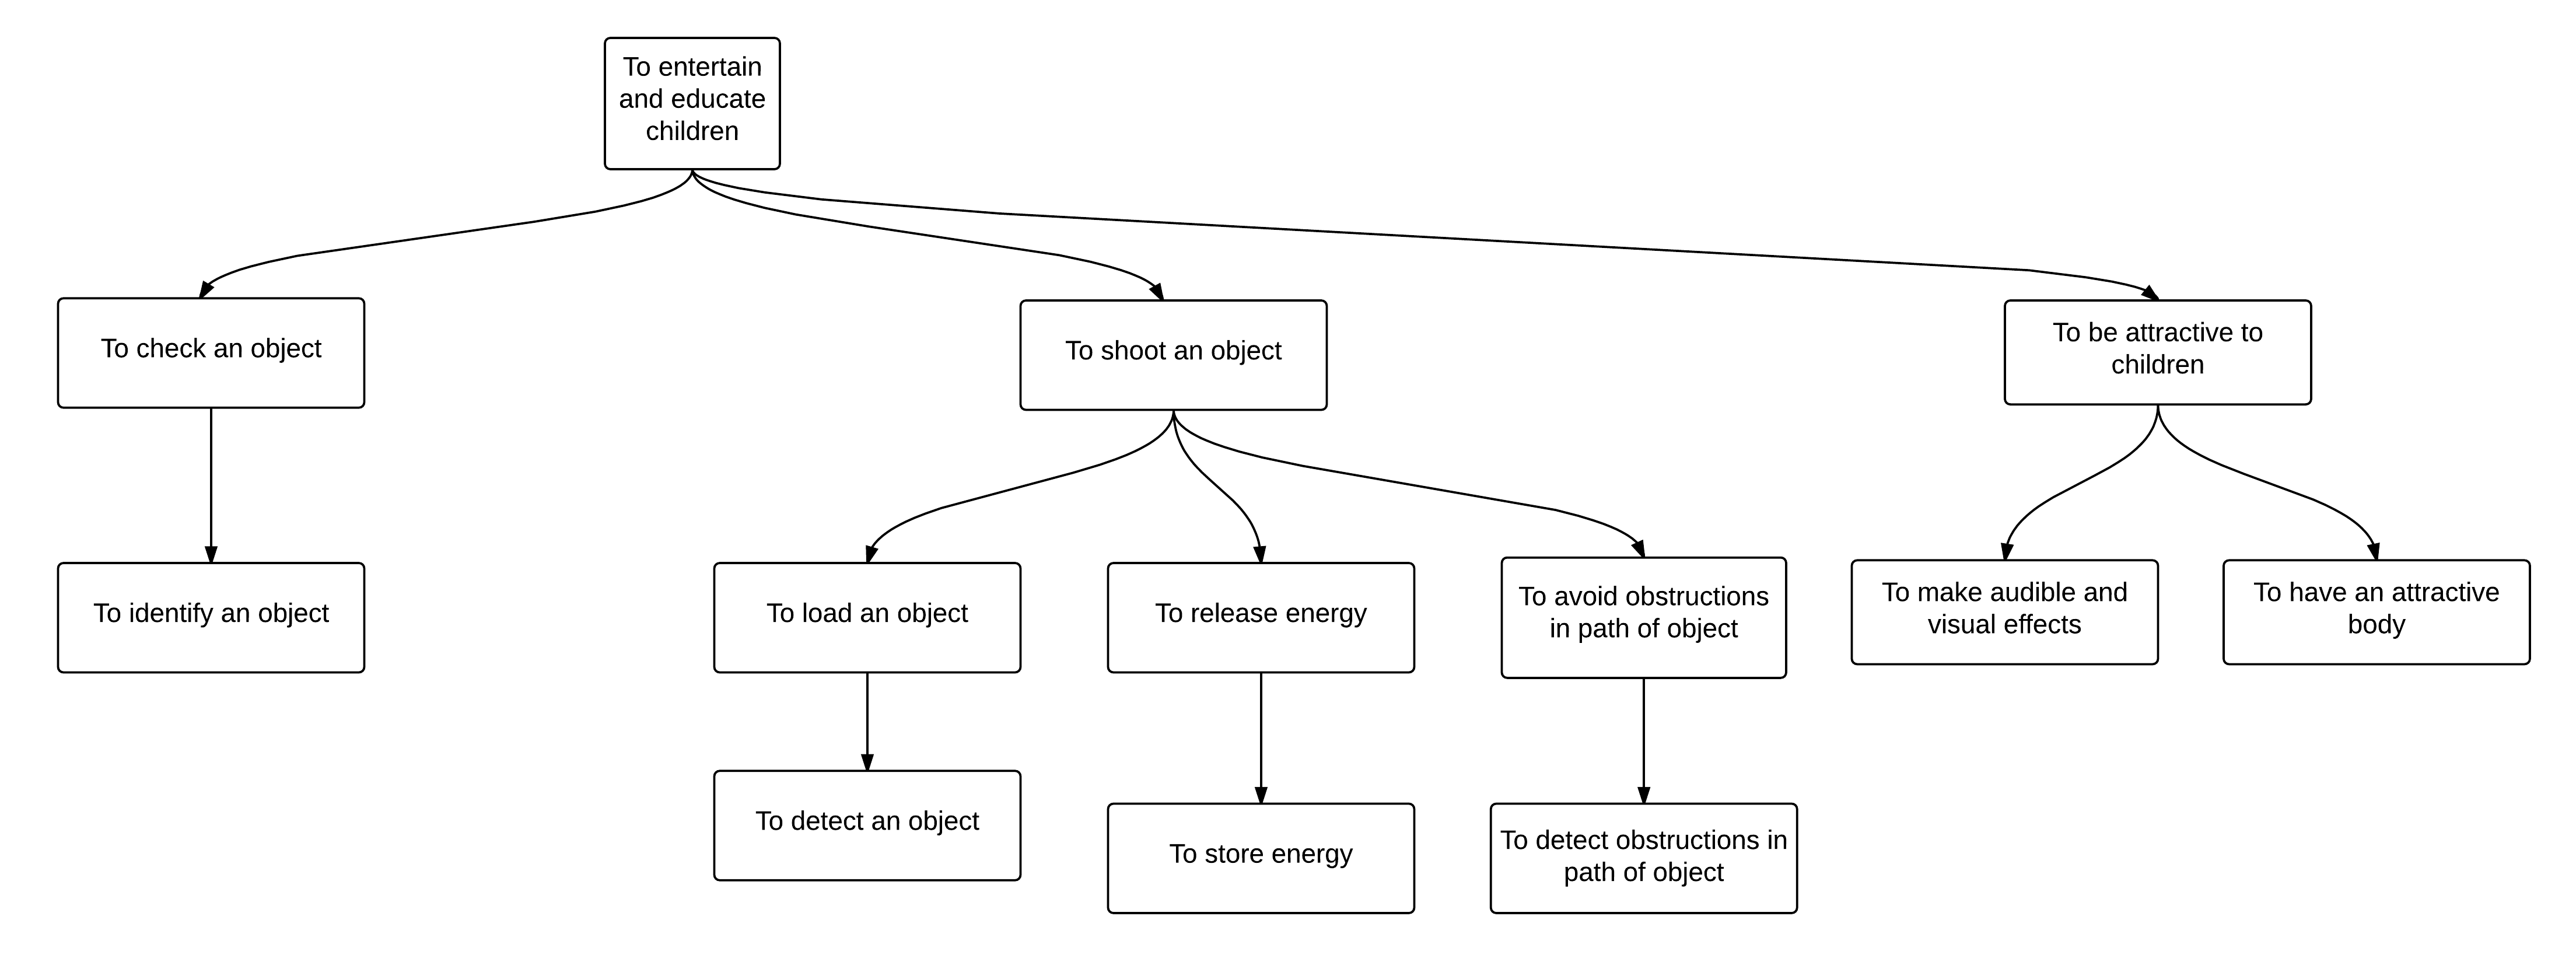
\includegraphics[width = 17cm]{Images/FunctionalAnalysis.png}
\end{center}
\caption{Functional Analysis}
\label{fig:FuncAnal}
\end{figure}

\chapter{MoSCoW analysis}
The requirements of the robot will be organized using the MoSCoW Analysis. The analysis can be found in Appendix \ref{appendix:moscow}. \\
The MoSCoW Analysis will be used to pinpoint the requirements and differentiate the actual requirements from the more luxury objects. This will be useful when there is a time rush or a shortage in money for example. \\
The results of the MoSCoW Analysis and the Functional Analysis in the previous chapter, will be used to set the Morphological Map, which will be found in the next chapter.

\chapter{Morphological map}
Using the MoSCoW Model and the Functional Analysis of the previous chapters, the Morphological Map for the designs was made. This Morphological Map can be found in Table \ref{table:morphologicalmap}.

\begin{table}[h]

\begin{tabular}{llllll}
Subject            & Option 1          & Option 2   & Option 3     & Option 4     & Option 5          \\
                   &                   &            &              &              &                   \\
Mechanical Parts   &                   &            &              &              &                   \\
                   &                   &            &              &              &                   \\
Movement           & 3-wheel           & Tracks     & 4-wheel      & None         &                   \\
Release Mechanism  & Spring            & Flywheel   & Air Pressure & Magnetic     & Turning + gravity \\
Shootable Objects  & Balls             & Cubes      & Anything     &              &                   \\
Protection         & Material          & Case       & Structure    & Frame        & Bumper            \\
Design             & Turtle            & Dragon     & Robot        & Truck        & Whale             \\
                   &                   &            &              &              &                   \\
Electronical Parts &                   &            &              &              &                   \\
                   &                   &            &              &              &                   \\
Sensor (Shooting)  & Ultrasonic        & Infrared   & Camera       & Laser        &                   \\
Computing          & Arduino           & Laptop     & Raspberry Pi & Mobile phone &                   \\
Recognition Object & RFID              & Camera     & Radio        & Magnetic     & Infrared          \\
Obstacle avoidance & None              & Ultrasonic & Camera       & Laser        &                   \\
Battery            & Plugged in & Li-Ion     & LiPo         & NiMH         &                   \\
Display				& None & LCD & & & \\
Speakers 			& Yes & No & & & 
\end{tabular}

\caption{Morphological map}
\label{table:morphologicalmap}
\end{table}
The Morphological Map is divided into two parts: the Mechanical parts and the Electronical parts. The Mechanical parts will be varied when making the initial designs, while the Electronical parts will remain constant, as the initial design of the robot will unlikely affect the electronical parts, since the overall electronics design of a small scale robot is usually the same. \\
There are a few little things to note about the Morphological map. The first one being that sensor (shooting) is the sensor that is used to prevent the robot from shooting when the child is right above the shooting mechanism. This will ensure the safety of the child. \\
This map will be used to create a certain amount of initial designs, of which three shall be selected to be improved and turned into full concepts.


\chapter{Object design}
The objects that can be used in the robots come in different forms and sizes. The form and size of these objects will be decided in the following paragraphs. 

\subsubsection{Form}
Theoretically, one can consider all kinds of forms for the objects. However, this robot would need to transport the objects and shoot them into the air. This is realized in an easy way by taking spherical objects. Balls are able to roll with low friction and are easily transported through the robot. Square objects for example won\rq{}t be able to transport as easily as spherical objects would. \\
For these reasons, we have decided on using spheres as the final form.

\subsubsection{Size}
Safety is a big issue regarding the size of the balls. Children under 3 years of age can safely play with balls that are at least 44 mm of diameter (\lq\lq{}Choosing Safe Toys\rq\rq{}, n.d.). The specific age group will be given in chapter \ref{chap:games}: The game. \\
Because of this, the balls will have to be at least 44 mm. Besides this, the readability of the print on the ball, the availability of that certain size of balls and the amount of space used for the loading cylinder, where the balls are stored, should be considered. \\
Balls should already be readable from 44mm, so this should be fine, but it would of course be more readable when selecting larger balls. \\
The easiest available balls to get are balls with a diameter of 50 or 60mm. Other balls would probably have to be specifically fabricated. \\
Finally, the available space for the loading cylinder is 180mm high and has a diameter of 155mm. When selecting 50mm, it would be enough space to store approximately 20-23 balls. Figure \ref{fig:balllaunch} shows how the balls are stacked. \\
\begin{figure}[H]
\begin{center}
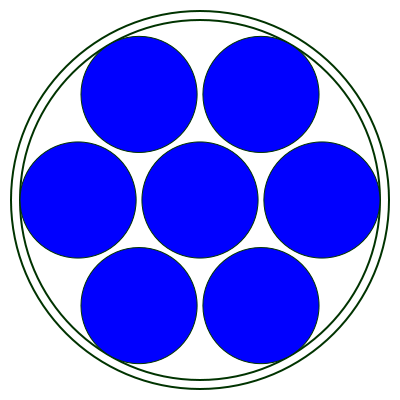
\includegraphics[width = 10cm]{Images/BallLaunch.png}
\caption{This figure shows how the balls will fall in the launching pipe for 50mm balls.}
\label{fig:balllaunch}
\end{center}
\end{figure}
If the 60mm balls would be used though, it would decrease significantly to around 12-15 balls. 
Since there is also storage space in the neck, the total storage would be around 30 balls. This is enough for the 26 letters of the alphabet and without using the neck it would be enough for 2 sets of the numbers 0-9. \\
The 50mm balls would be most advantageous and will therefore also be used. 

\subsubsection{Material}
For the materials, the ball must not be able to hurt the child when it falls on the childs head. For this reason, a material like foam or styrofoam would be ideal 
\newpage
\subsubsection{Conclusion}
The final decision is 50mm foam or styrofoam balls, depending on the availability and price of both. An example is shown in figure \ref{figure:lotteryball}.
\begin{figure}[H]
\begin{center}
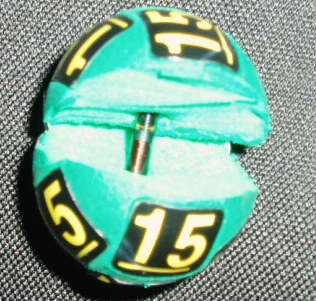
\includegraphics[width=10cm]{Images/LOTTERY-BALLS-with-rfid.jpg}
\end{center}
\caption{A 50mm foam ball}
\label{figure:lotteryball}
\end{figure}

\chapter{Initial design}
The design of the robot will be decided by doing a brainstorm. The brainstorm consists of three stages: first a lot of ideas will be generated, then the ideas will be discussed and to conclude the brainstorm, the ideas will be narrowed down to three concepts. The brainstorm technique and the ideas can be found in Appendix \ref{appendix:brainstorm}: Brainstorm initial designs. \\
The design of the game will not be elaborated here, this can be found in Chapter \ref{chap:games}: The game. The following are the three end concepts for the robot:

\section{Volcanobot}
\begin{wrapfigure}{r}{0.5\textwidth}
  \begin{center}
    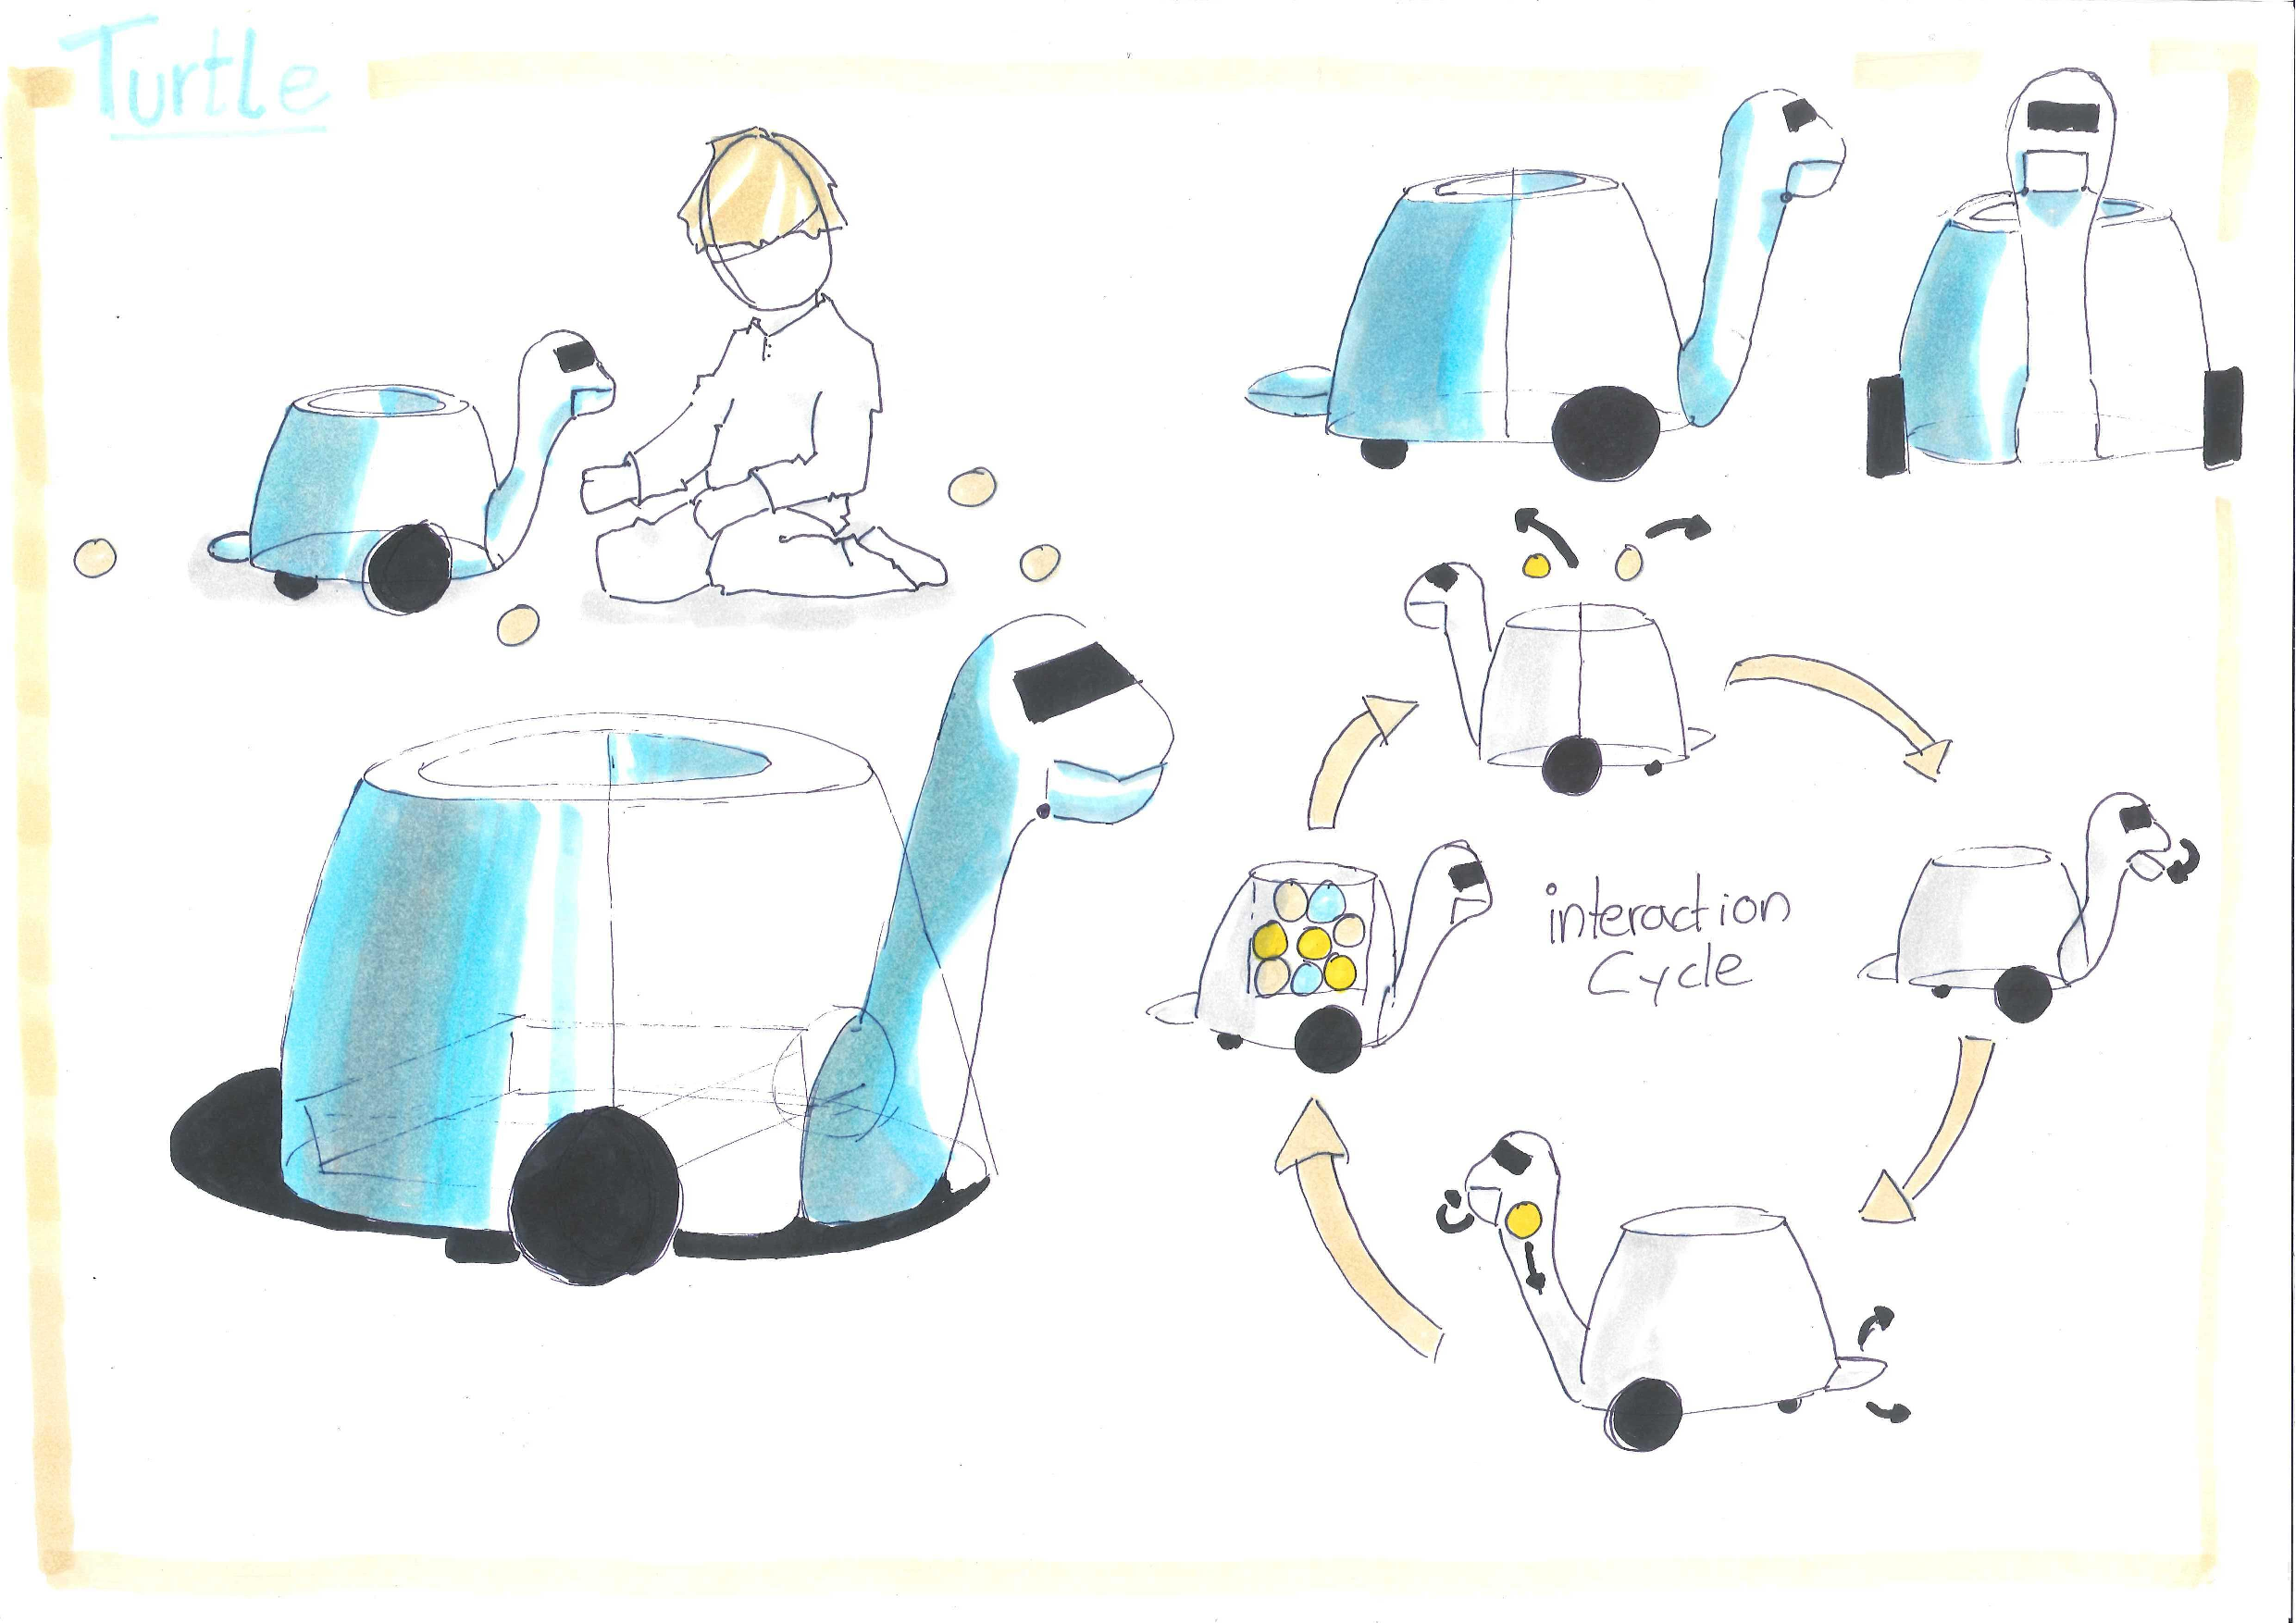
\includegraphics[width=0.48\textwidth]{Images/VolcanoBotConcept.pdf}
  \end{center}
  \caption{Volcanobot}
  \label{figure:volcanobot}
\end{wrapfigure}
The Volcanobot is a robot in the form of a tortoise with a volcano on its back, see figure \ref{figure:volcanobot}. The main idea is to let it shoot the objects from the volcano on its back, ask for a certain object, let the child retrieve that object and put it in the mouth to scan if it is correct. When all the items are retrieved, a new game will start by shooting all the objects out again.

Example: Volcanobot shoots the objects, asks for the answer of 3x3. The child then retrieves the ball with 9 on it and puts it in the mouth. It should scan the ball and swallow it and it will ask a new question. If the child retrieved the ball with 8 on it, the ball should fall out of its mouth or be spat out by the robot.

The robots shooting mechanism is based on a spring and would require a container for the objects with a radius of approximately 160mm and a height of 200 mm, for 20 balls with a 25mm radius. The container would be filled from a high point at a high angle, so that the objects can\rq{}t be shot back into the filling mechanism or get stuck in the filling mechanism. Because a tortoise neck is generally very low, we will have to use a mechanism similar to a conveyor belt to transport the object to the main container in the middle.

The robot will give feedback to the child when the objective is correctly solved or when it\rq{}s not. Feedback is given on a screen in the robots eyes and via movement and sound. When the child makes a mistake he or she will be encouraged to try again.

\section{Box-bot}
\begin{wrapfigure}{l}{0.5\textwidth}
  \begin{center}
    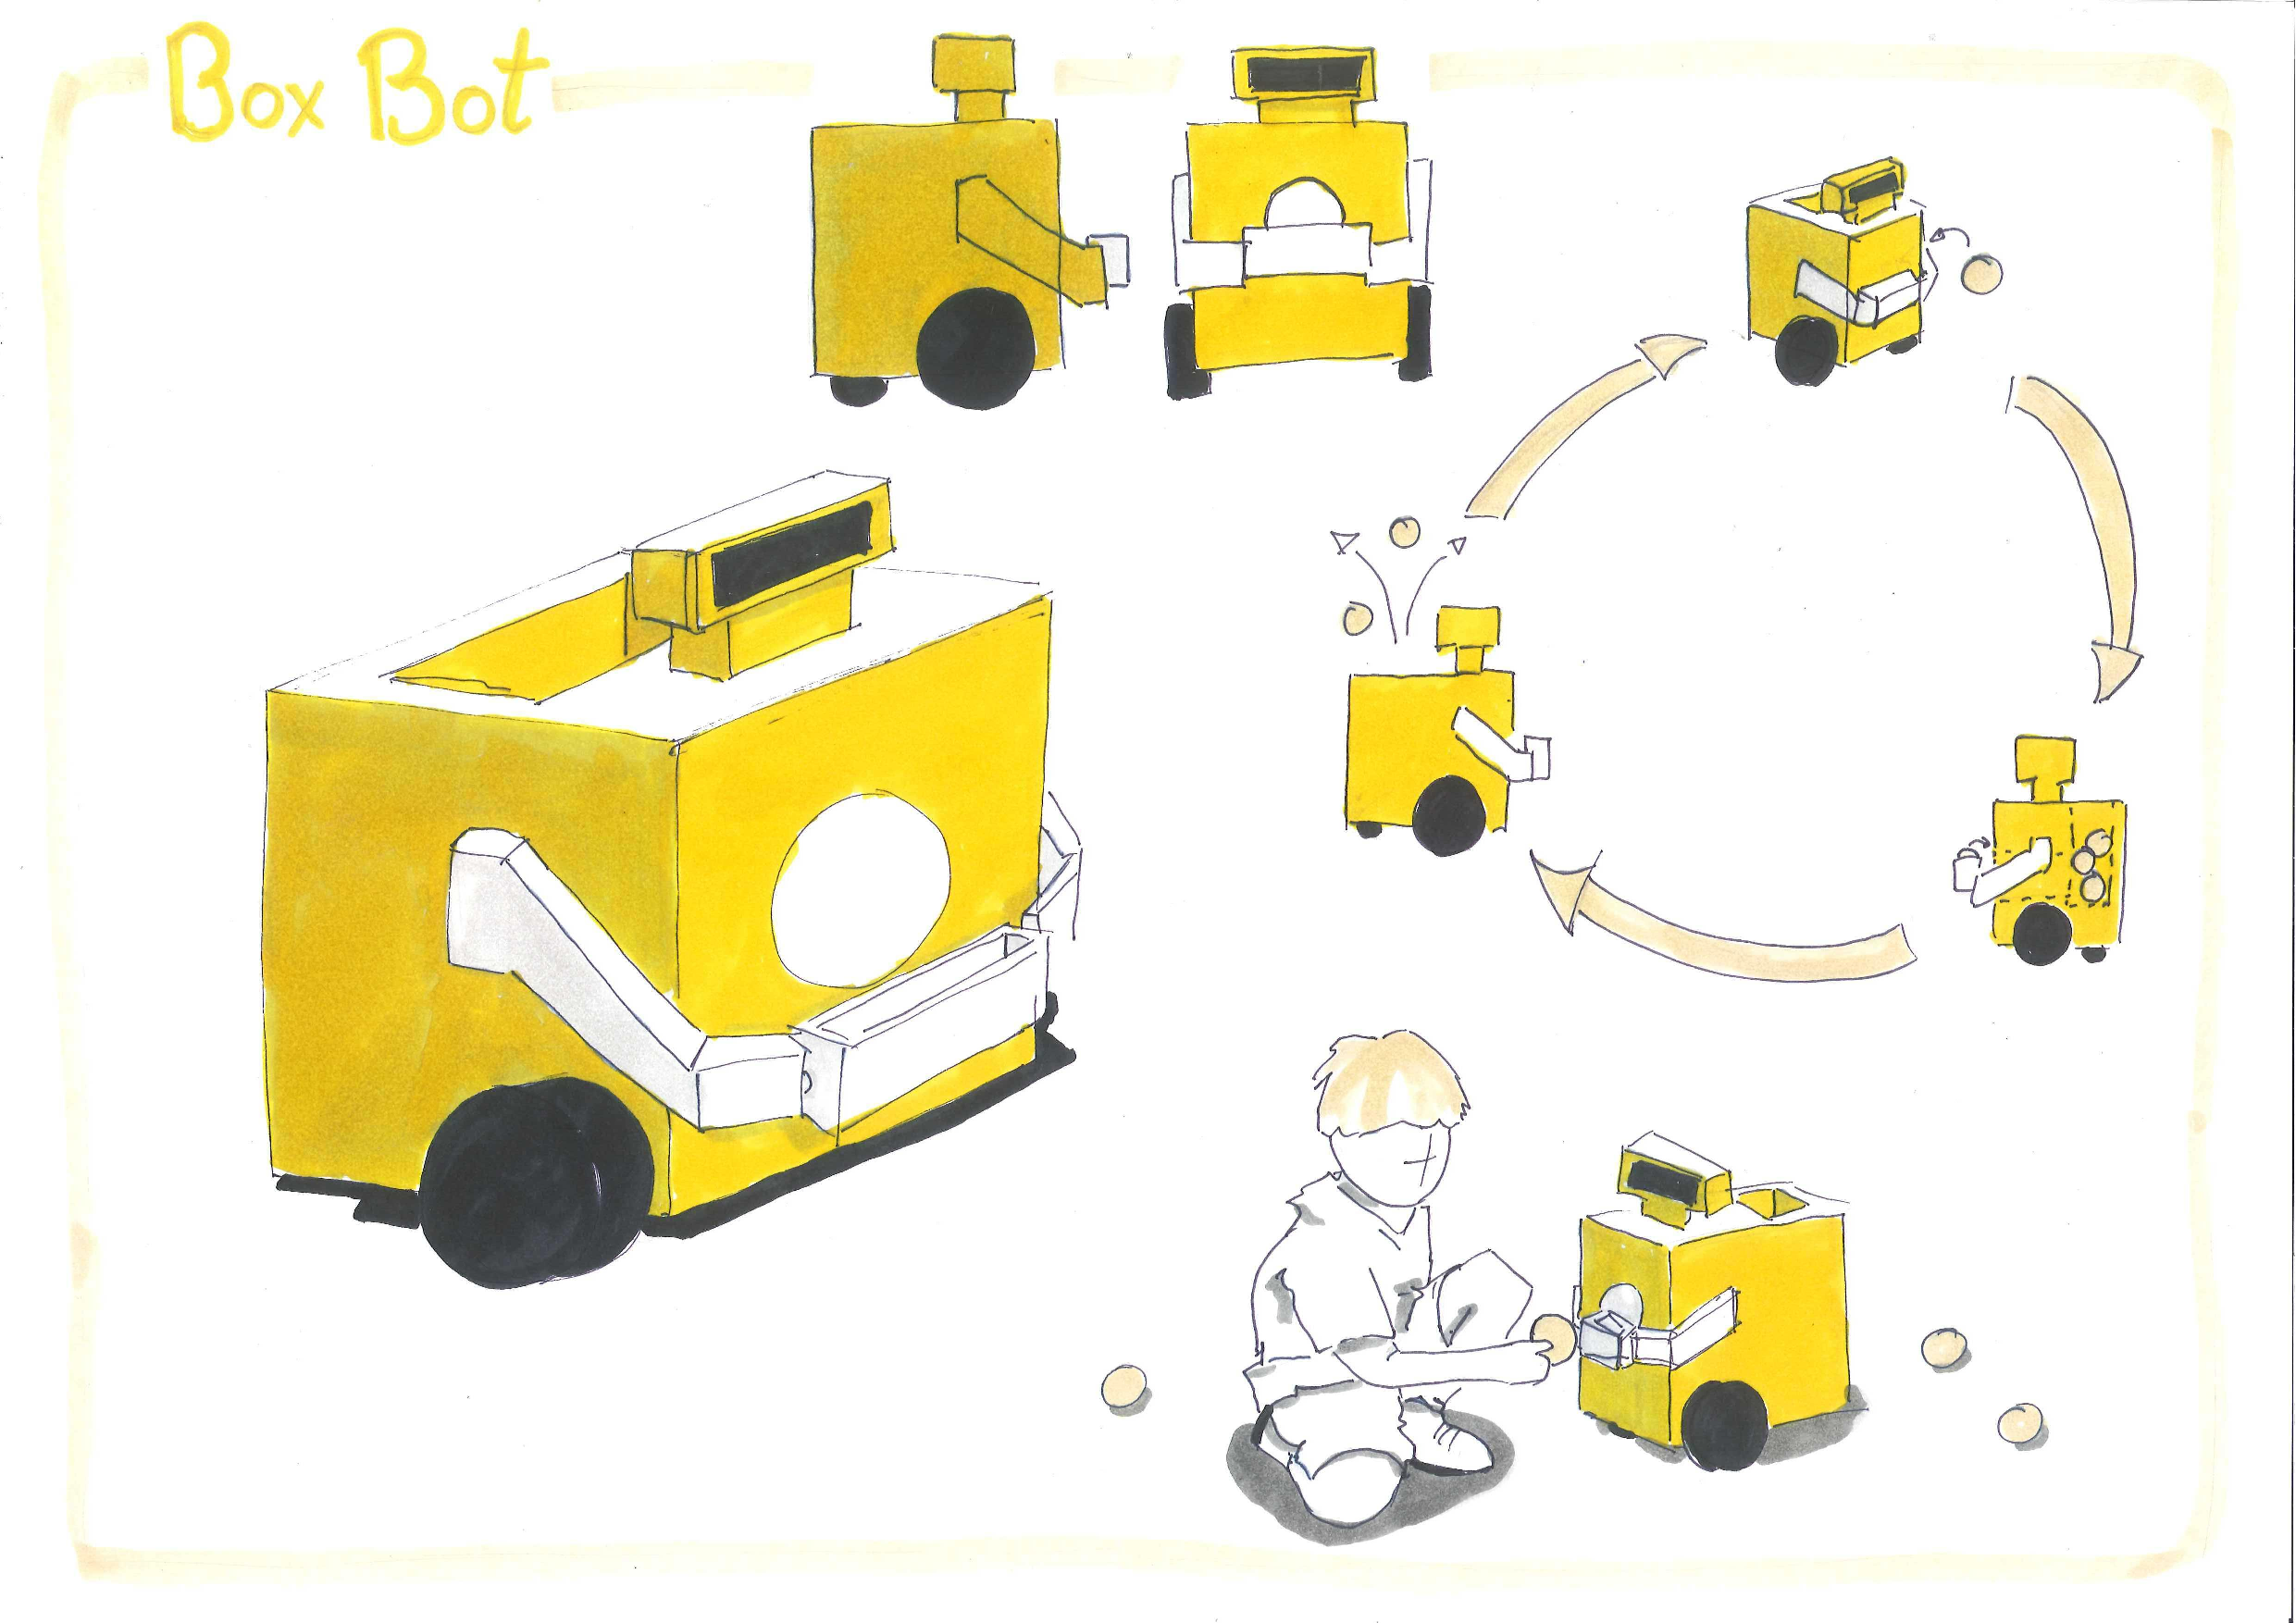
\includegraphics[width=0.48\textwidth]{Images/BoxBotConcept.pdf}
  \end{center}
  \caption{Box-bot}
  \label{figure:boxbot}
\end{wrapfigure}
The Box-bot is a square formed robot, see Figure \ref{figure:boxbot} . The game begins by shooting from the top of the robot and would ask for a certain object via sound and a screen. The child retrieves the object and puts it in a hole on the front side of the robot to scan it. If it\rq{}s correct, it will be swallowed and kept in its container. If it is not right it would be dropped on the ground in front of the robot.

The shooting mechanism would be similar to the Volcano-bot, using a spring and a container for the objects with a radius of approximately 160mm and a height of 200mm, for balls with a 20mm radius. It would also have to be filled from a high point at a high angle, so the objects can\rq{}t shoot back into the filling mechanism or get stuck in the filling mechanism. However, the exterior of the Box-bot won\rq{}t require a low loading point, like the Volcano would, so it\rq{}s possible to load from a higher point, without needing a conveyor belt mechanism.

\section{Truck Teacher}
\begin{wrapfigure}{r}{0.5\textwidth}
  \begin{center}
    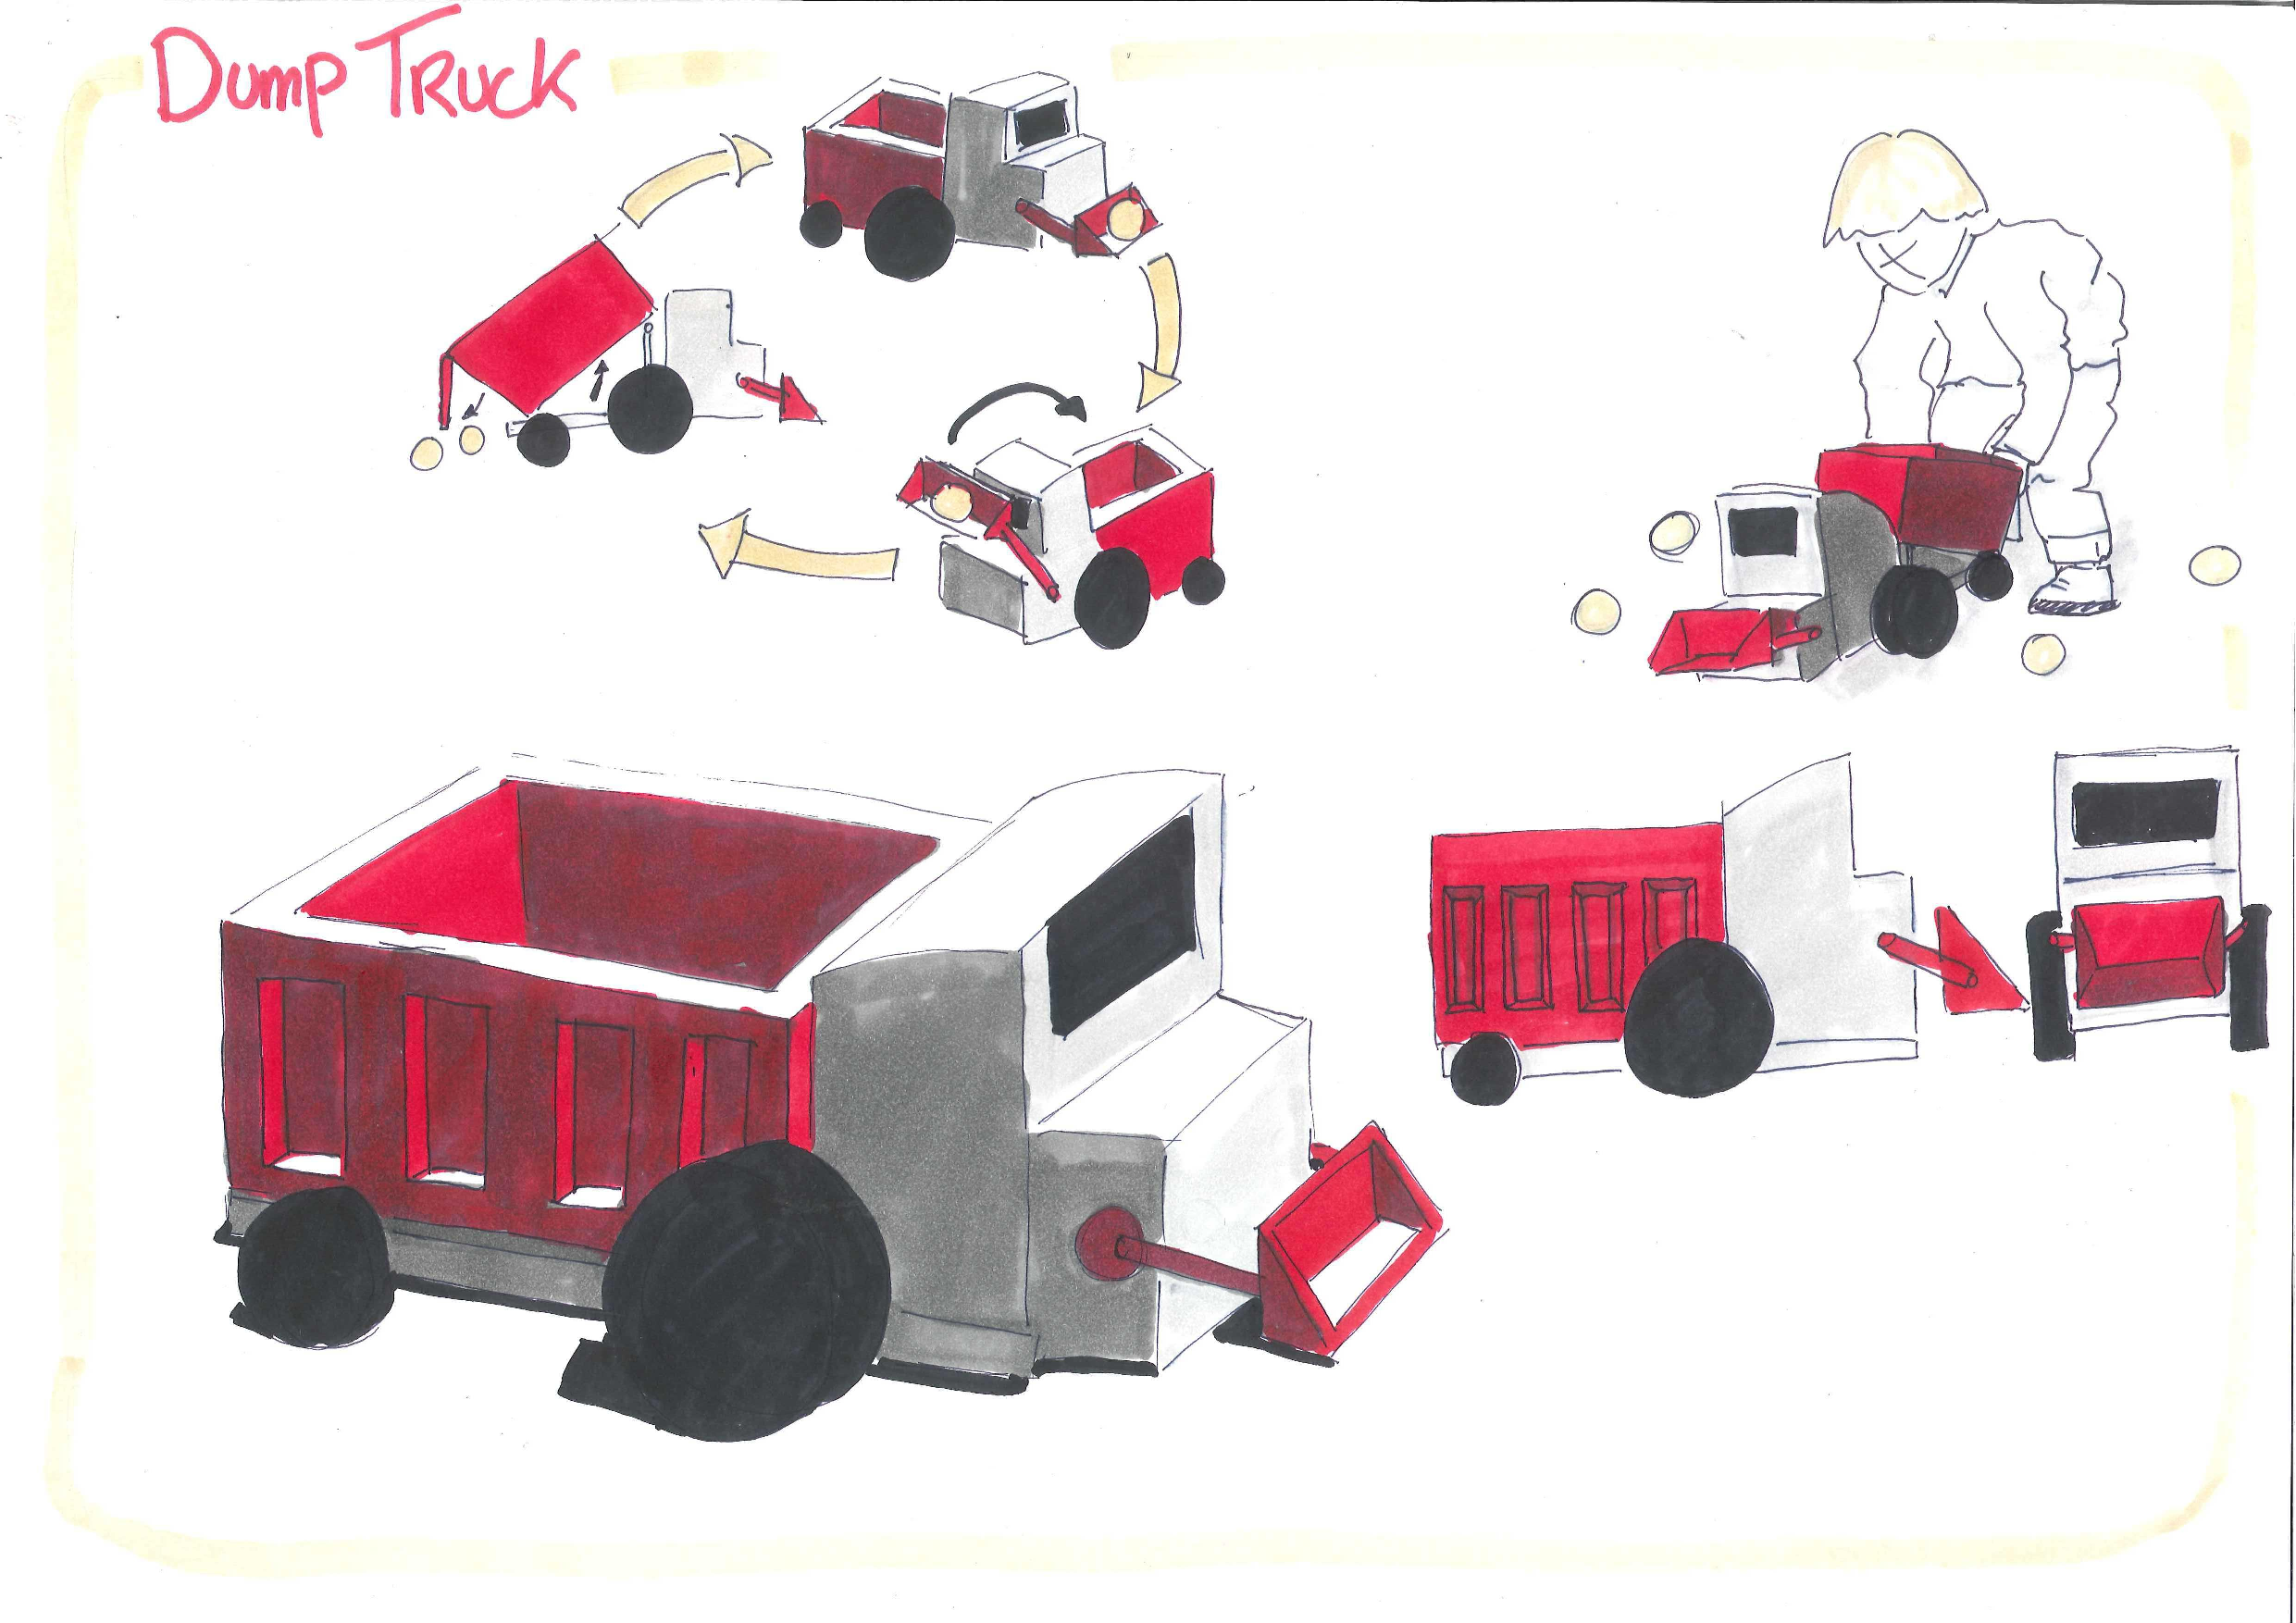
\includegraphics[width=0.48\textwidth]{Images/TruckTeacherConcept.pdf}
  \end{center}
  \caption{Truck Teacher}
  \label{figure:truckteacher}
\end{wrapfigure}
The Truck Teacher is a robot in the form of a shovel truck, that can be found in figure \ref{figure:truckteacher}. At the beginning of the game, it lets the balls roll off the truck by toppling the container. Then the robot will ask for a certain object. The child should then retrieve the object and scan it on the window or in the bucket of the truck. If it is the correct item, it will load the object into the container of the truck by rotating the arm of the bucket.

This robot would release the balls by toppling the container by using a screw spindle. The container would be the same size as the platform and the objects would have to be balls, since lower friction is needed to let the objects fall of the truck.

\chapter{The game}
\label{chap:games}

\section{Initial Game Choice}
The robots main purpose is to play a game or several games with a young child. Several games were designed. The following list consists of all considered games and a conclusion on how feasible and unique they are.
\subsection{Tag}
Playing \lq\lq{}Tag\rq\rq{} with the child. This consists of the child touching the robot, the child starts to run away, the robot will then try to touch the child, the robot will try to run away and so on.
This game would give a lot of difficulties: the robot has to be very fast, the child needs to be detected and very important is that the robot would not be scary for the child, since the robot will run after them. This game was not chosen, since the robot will be quite heavy and fast, so it would be too dangerous for the child to be run over or bumped in to.
\subsection{Ball shooting game 1}
This was a spin-off of the \lq\lq{}Tag\rq\rq{} game. The robot would shoot a ball and then would drive away from the ball. The child would need to retrieve the ball and put it back in the robot. This gave the same complication as the \lq\lq{}Tag\rq\rq{} game and this idea was discarded in kind.
\subsection{Hide and Seek}
This game would have two variants, one where the robot seeks the child and one where the child looks for the robot. When the robot needs to hide, it would need excellent detection properties to see if it is hidden. The detection was considered to difficult to build in half a year so the idea was not considered feasible.
\subsection{Tamagotchi}
In this game the child would need to care for the robot, feeding it, playing with it and letting it sleep. This would teach the child caring for something. The robot would have to be excellent in reacting to the child and for this it would need touching sensors and multiple moving parts. A lot of caring robots are already on the market, like for example Pleo (see Appendix \ref{appendix:competitors}: competitors), so it would not be new or innovating. Considering this, the Tamagotchi game was not chosen.
\subsection{Dancing}
The design was to include a dancing feature in the Tamagotchi game, but it would also be very fun just to have an extra feature for the robot. The robot will begin to dance when it hears music. The robot would need music detection and would need to have several dance moves. This is quite easy to implement with easy sensors, so this feature is feasible.
\subsection{Manual driving}
Manual play with a controller can also be very fun, but it\rq{}s not part of the project, since it needs to be an autonomous robot. This feature might be implemented along the development for testing purposes, but is not deemed necessary for a successful product.
\subsection{Ball shooting game 2}
The ball shooting game was slightly adjusted to make it a feasible game. The ball would have a picture on it and the robot would ask for the correct ball. The child would then return the correct ball to the robot and the robot would somehow collect these in his body. When the robot has collected all the balls it will shoot them out of his body again, and the game will start over. This game can have several elements for different ages, for example by using colored balls, balls with letters, balls with numbers etc. \\
\lq\lq{}Ball shooting game 2\rq\rq{} is considered feasible since it doesn\rq{}t involve the difficulties of \lq\lq{}ball shooting game 1\rq\rq{} , like fast driving and following an object anymore. \lq\lq{}Ball shooting game 2\rq\rq{} is considered more original and fun for a large span of age groups.
\subsection{Conclusion}
The robot will be used for ball shooting game 2 as explained above and as  and dancing to music could be implemented as an extra feature. This is considered a feasible game, which can entertain the child for a long time and keep it entertaining for several years if the robot and the game are designed correctly.


\section{Game options}
The selected ball shooting game is also very expandable. Following is a list of possibilities for the object requesting education robot. \\

Forms of recognition:
\begin{itemize}
\item Colour
\item Form
\item Animals
\item Food
\end{itemize}
Math:
\begin{itemize}
\item Multiplying
\item Subtracting
\item Adding
\item Dividing
\end{itemize}
Alternate options:
\begin{itemize}
\item Driving manually
\item Dancing with music
\item Tamagotchi 
\item Walking autonomously
\item Sleep
\item Dance while playing

\end{itemize}

\chapter{Improve 3 initial designs}
\section{Proof of concept calculations}
\section{Sketches of exterior}
\section{Sketches of mechanics}
\section{Initial software architecture}
\section{initial electronic and electrical design}

\chapter{Concept choice}
In this chapter, the decision for the final concept design will be made and explained. Recall that there were three concepts: the Truck Teacher, the Box-Bot and the Volcano Robot. The decision was made after careful consideration of the following factors:
\begin{itemize}
\item Difficulty to build
\item Entertainment value for children
\item Originality
\end{itemize}
\section{Difficulty to build}
The final concept should not take half a year to build, because there is only 8 weeks. This is an important factor, but all of the concepts tick the box of “able to be constructed in less than 8 weeks”. The “Truck Teacher” is the easiest to build. There would be only 2 very simple constructions besides the driving features:
\begin{itemize}
\item Making the container on the back able to dump balls.
\item Making the bucket on the rotate to get the balls into the back container.
\end{itemize}
The Box-bot and the Volcanobot both require some more construction to be fully functional.
\begin{itemize}
\item A launching mechanism with a spring, an air-cannon or something else.
\item A conveyor belt to transport the balls, once they have entered the robot, to the launching tube.
\end{itemize}
For the Volcano Robot, an appealing shell is also required, which requires the making of a jig. The Volcano Robot is therefore the hardest to build, followed shortly by the Box-Bot and the Truck Teacher. The Truck Teacher being the easiest to build.
\section{Entertainment value for children}
After meeting with Maja Rudinac, expert on robots and their interaction with children, it became clear that the Truck Teacher concept would not be very interesting because there is already a high number toys in the form of a truck on the market. A toy can be entertaining if they already know it, but a toy like they have never seen before is likely to be more entertaining, engaging. \\
The Box Bot is very simple and whilst it may look like it is from the future, it’s not a very attractive concept for children. Adding a lot of lighting and sound effects might increase this, but not in the way that a different body shape would affect it.\\
Miss Rudinac also mentioned that she had never before seen a robot shaped like a turtle with a volcano on its back. After some research, this turned out to be true. There is however a character from the Pokémon [Nintendo, 2014] named Torkoal that looks very similar to the concept of Volcano Robot.\\
The entertainment value of Volcano Robot is the highest, followed by the Truck Teacher and the least attractive robot is the Box Bot.
\section{Originality}
Making a robot that is original is not very important, but it makes for that “never seen before” experience with children. An original and new concept that does not exist yet adds to the entertaining value for children. You could therefore call originality a sub-category of the entertainment value.\\
As mentioned in the previous paragraph, Volcano Robot scores high when it comes to originality. Both the Box-Bot and the Truck Teacher score low, but the Truck Teacher scores the lowest. This is because a truck like toy has been seen numerous times before.
\section{Final concept choice}
After weighing the pros and cons of all the concepts against each other, the Volcano Robot concept comes out as the best. Volcano Robot scores high on originality and entertainment value. Even though Volcano Robot might be a bit harder to design and build, it will be more interesting and is probably more fun for children. Therefore the Volcano Robot was chosen to be further developed.
\chapter{Name and logo}
Several options were considered for the name of the turtle. First of all the name needs to appeal to children and their parents. It would be best to have a short name, which is easy to pronounce. Furthermore the name needs to relate to the robot, so it has to do something with volcanoes, turtles, robots or child education.\\ 
After searching for names the island group Tawi Tawi was found in the Philippines. This island group has several volcanoes and an island called Turtle Island. It was decided that Tawi Tawi sounded nice but was a little bit too long, so the name would be shortened to Tawi. Tawi the Turtle has a nice ring to it and is a unique name for the robot.\\ 
After deciding on the name a logo was designed. The logo (see figure \ref{fig:logo}) is very simple so it is easy to recognize for children and their parents.
\begin{figure}[H]
\begin{center}

\includegraphics[width = 10cm]{Images/logo_Tawi.png}
\caption{The logo for Tawi}
\label{fig:logo}
\end{center}
\end{figure}

\chapter{Development prototype design}

\section{Analysis of required parts}

\section{Mechanical design}
\subsection{The ball transport system }
In the robot, spherical objects need to be transported from the lower part of the neck to the upper part of the launching pipe. There are multiple solutions to this problem. First let’s start with the requirements for this problem. The objects that needs to be transported are styrofoam balls with a weight that is one or two grams. The solution must also be small in height to make sure that the robot is as low as possible.  \\
It was considered to use a shooting system that shoots the balls through a pipe into the launching pipe. This would involve a similar system as used in the launching pipe itself; a spring that stores the energy and a rack and pinion construction. A system like this is complex and it would not be easy to calculate the friction between the spherical objects and the walls of the pipe.\\
\\
Another solution was a conveyer belt to transport the spherical objects. This belt could be a V belt or a timing belt. V belt pulleys are bigger in diameter than timing belt pulleys, and the whole solution would also be more expensive than a timing belt setup. So the solution comes to a timing belt with pulley.\\
\\
In figure \ref{figure:balltransport} , a drawing is displayed which shows the timing belt pulley setup. Now, a calculation of the torque of the motor to transport the balls is made.\\
\\The torque that needs to transmitted to the driving pulley (the upper pulley in picture xxx) is equal to: \[M=\frac{T_{e}*d_{p}}{2c}  \].
The effective tension is equal to:
\[T_{e}=F_{a}+F_{g}+F_{ab}+F_{ai}  \]
$F_{a}$ is the resulting force from acceleration of the balls. $F_{g}$ is the resulting force of the weight of the balls. $F_{ab}$ is the force resulting from acceleration of the belt and $F_{­ai}$ the force required to accelerate the pulley.  There is also friction from the fact that the rubber strips that hold the balls are colliding with the launching pipe. It is now stated that the acceleration is almost zero and only the steady state situation is regarded. Then, only the weight of the balls is important. There is room for five balls at once, so the total weight is 10 grams. With the angle included (56.37 degrees) this results in a tension force of 0.1 N. The total moment the motor will have to deliver, with a pitch diameter of 0.02 meter is 1 Nmm. The friction from the flaps is hard to calculate. We will assume that the total moment to be delivered is 10 ten times this, so 1 Ncm. It is accepted that the balls will travel the 0.25 meter along the belt in 10 seconds. With the pitch diameter of the pulley, this results in axle speed 24 rpm. The selected motor which is properly available has a no load speed of 25 rpm, and a rated torque of 8 Ncm. This motor will operate at near no load speed, because the moment required is much lower than the rated torque, so the 24 rpm will most likely be reached and the ball will be transported in just over 10 seconds. 
\subsection{Neck strength calculations}
To check whether the neck is strong enough to support a child pulling on it, a strength calculation is necessary. The material used is pvc, with yield strength of 35 MPa (DYNA, 2003).
The maximum moment which the pipe can hold is:
\[M=W*\sigma\]
With
\[\frac{\Pi}{32}*\frac{(D^{4}-d^{4})}{D}\]
The outer diameter $D$ is 63 mm, and the inner diameter $d$ is 59 mm. So $W$ is 5665 mm3. The maximum moment that can be imposed is $35*5665= 2.0*10^5$ Nmm. 
The free neck length is $112 mm$, so the maximum force to be imposed $2.0*10^5/112 = 1770$ N. This equals a pull force of $180 kg$ in perpendicular direction of the neck. Conclusion: this is enough to support a child pulling it. How much force the robot can sustain before it tips over will be calculated in  \ref{sect: mechanical design: center of mass(or something like that)} 


\section{SolidWorks model}
\section{Software architecture}
The most important scenario for the robot is that the robot can ask for a ball, then wait for the correct ball to be inserted and give positive or negative feedback depending on whether the given ball was correct. After repeating this process until the volcano fills up, the robot erupts, spreading the balls around himself again. \\
The overall architecture of the robot is that one central node (“robot”), that delegates work towards several lower level nodes, that in turn each listen to an even lower level node, which either repeats to process or directly controls a device. \\
With this structure in mind the classes can be defined. Figures \ref{fig:controllers} The first subsystem is the overarching group that contains the handlers for the lower level functions. Figure X+1 shows the handlers for each node in the first two rows of Figure \ref{fig:FuncAnal}. The Audio and Video are separated into their own classes to create a distinction of responsibility for each class. 

\begin{figure}[!htb]
\begin{center}
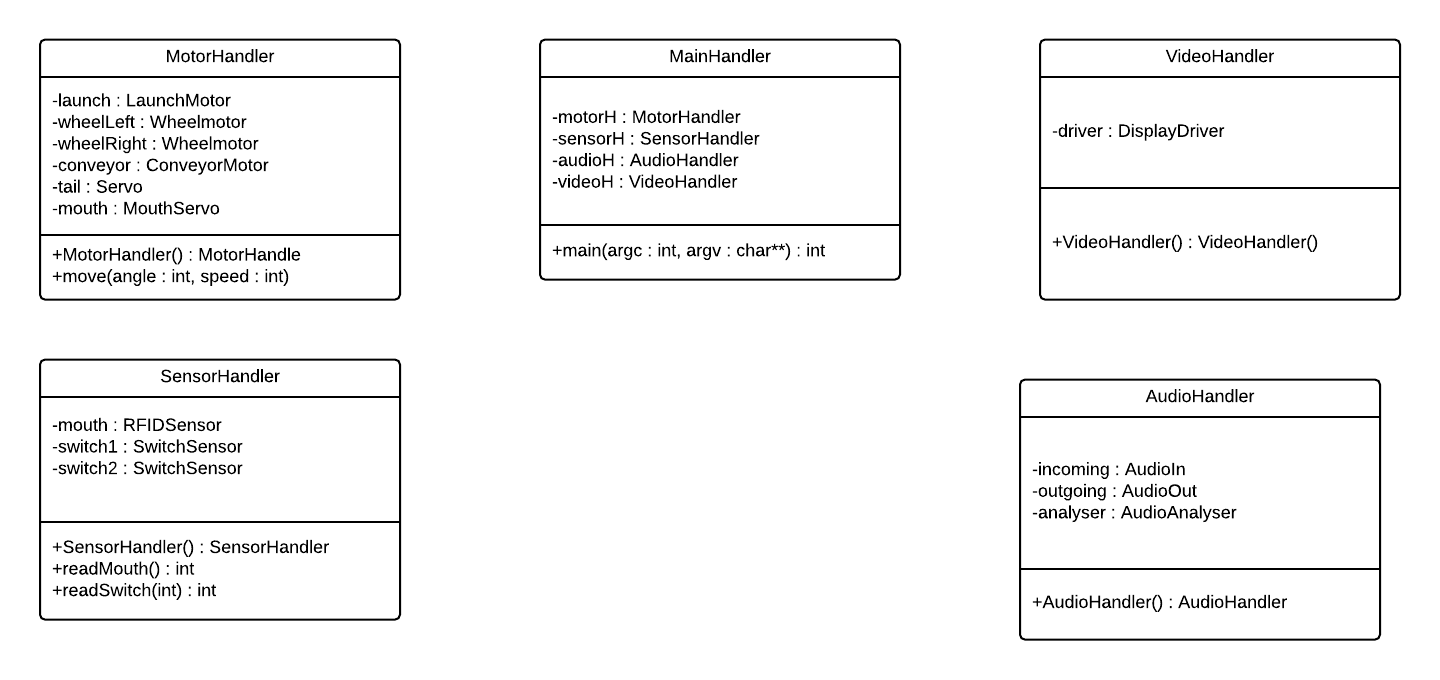
\includegraphics[scale=0.40, angle=90]{Images/VolcanoBot-Controllers.png}
\caption{The first subsystem is the overarching group that contains the handlers for the lower level functions. These are the The Audio and Video are separated into their own classes to create a distinction of responsibility for each class.}
\label{fig:controllers}
\end{center}
\end{figure}
\begin{figure}[!htb]
\begin{center}
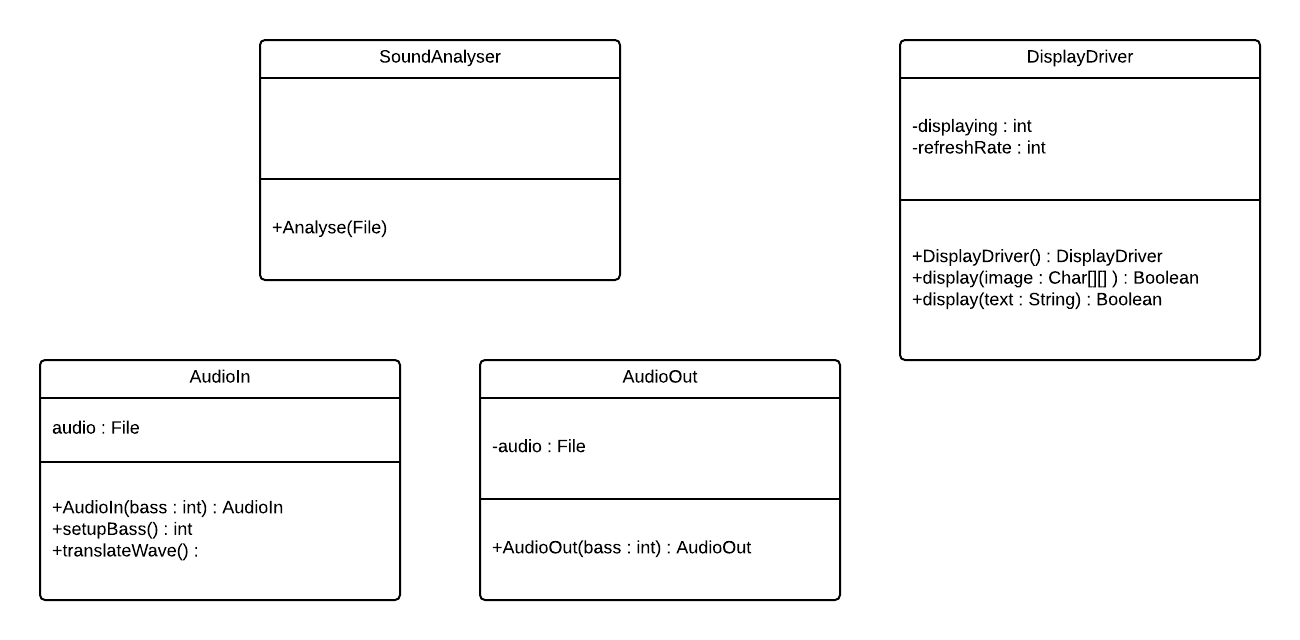
\includegraphics[scale=0.40, angle=90]{Images/VolcanoBot-Audio-Video.png}
\caption{depicts the general idea for handling audio input and output. This has to stay ambiguous, since the actual functions and variables are highly dependent on what audio framework is compatible with the hardware of the robot, as well as the algorithm used to analyze and process the signal to and from the audio hardware.}
\label{fig:audiovideo}
\end{center}
\end{figure}
\begin{figure}[!htb]
\begin{center}
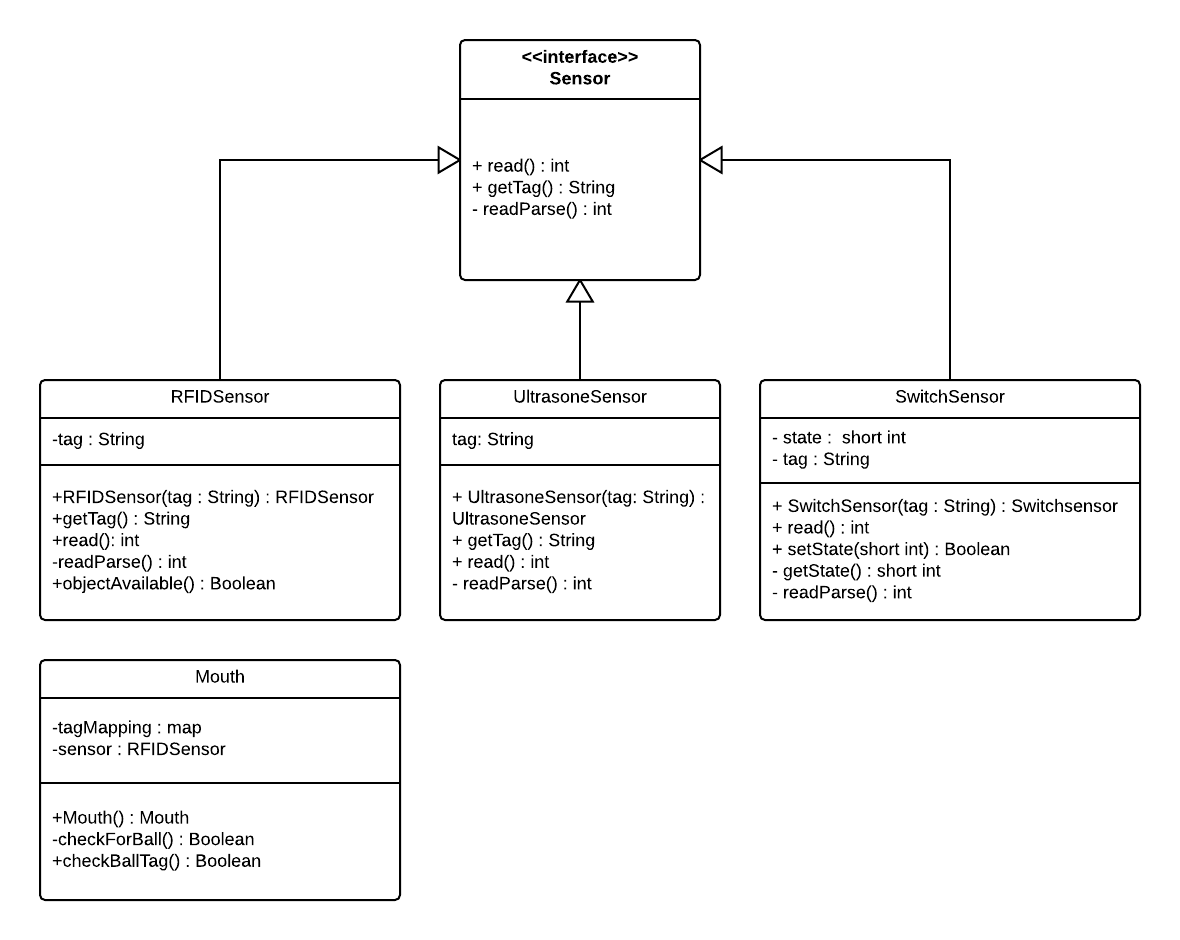
\includegraphics[scale=0.40, angle=90]{Images/VolcanoBot-ObjectScanning.png}
\caption{This figure shows the handling of balls given to the robot, in addition to other sensors used in the robot. The sensors make use of the interface “Sensor” to force consistent code patterns in every sensor implementation
}
\label{fig:sensors}
\end{center}
\end{figure}
\begin{figure}[!htb]
\begin{center}
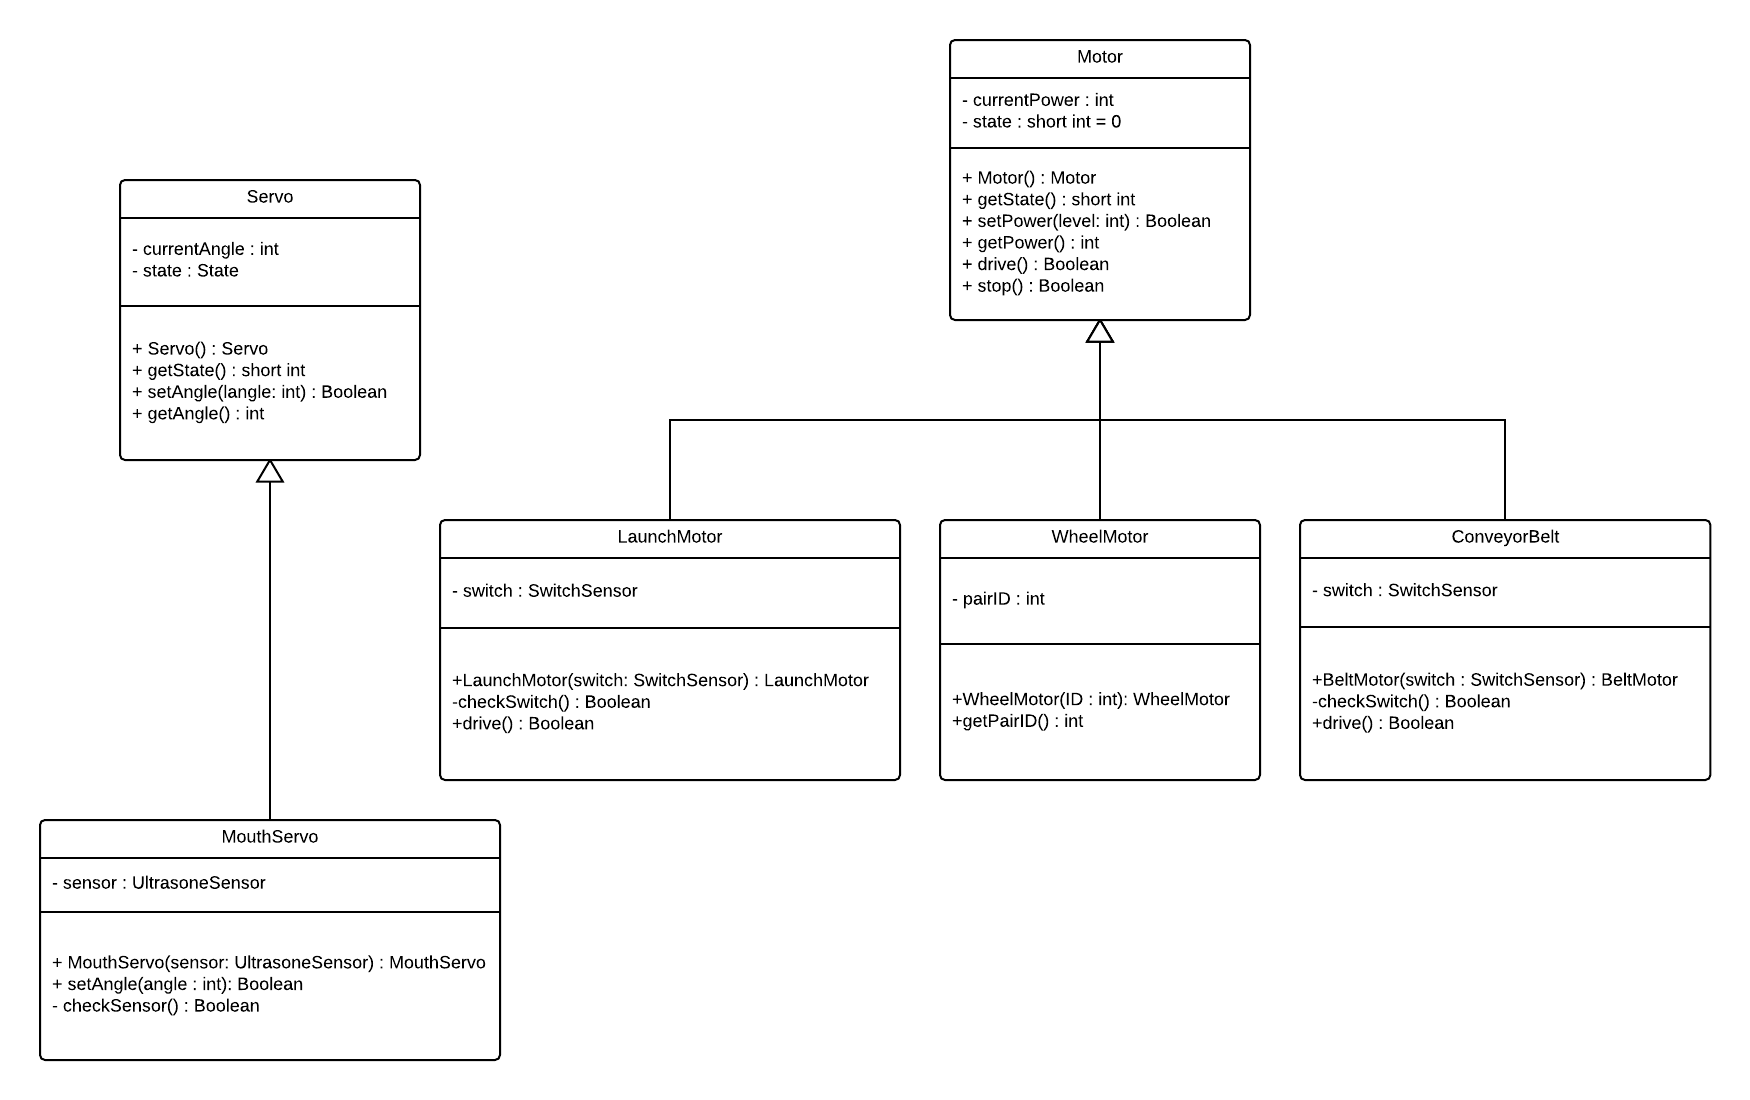
\includegraphics[scale=0.35, angle=90]{Images/VolcanoBot-Motors.png}
\caption{The last figure of this segment shows the regulations of the motors and servo. Again classes that handle a motor extend a parent class Motor to reduce duplicate code.}
\label{fig:motors}
\end{center}
\end{figure}

\section{Electrical and electronic design}
\subsection{Battery choice}
\subsubsection{Type of battery}
When choosing the battery, three types will be considered: Lithium-Ion, Nickel Metal Hydride and Lead batteries. To start off, Lead batteries are not considered viable, because of the low energy density and the size of the batteries (“Lead Based Batteries”, n.d.). The low energy density makes it heavy, while Li-Ion and NiMH can have the same capacity while they are lighter and smaller. Since the robot is supposed to be small, the lead batteries will not be used. 
\subsubsection{Li-Ion vs NiMH}
The advantages of Lithium Ion batteries (“Lithium Based Batteries”, n.d.) opposed to NiMH batteries (“Nickel Based Batteries”, n.d.) will be summed up here:
Advantages Li-ion over NiMH
\begin{itemize}
\item No memory effect like NiMH.
\item Higher power-density
\item No maintenance required
\item NiMH loses capacity when overcharged. Requires a special charging circuit to prevent this.
\item NiMH has a higher self-discharge rate than Li-Ion
\end{itemize}
Advantages NiMH over Li-ion:
\begin{itemize}
\item Faster charging
\item Li-ion can burst into fire when overcharged or overheated. Requires a special protection circuit. 
\item Li-ion starts losing capacity from the day it’s fabricated
\end{itemize}
The memory effect means that Nickel based batteries, when constantly discharged until a certain point, can “forget” it can discharge even further than that.  This can be cured by fully discharging the battery once in a while. It’s the NiCd battery that mainly suffers from this though and the NiMH batteries don’t suffer  from it that much anymore. Also, it mainly occurs when the batteries are always discharged until the same point, which is usually not the case for consumer technology.\\ 
Lithium Ion batteries are quite similar to NiMH batteries, but Li-ion has a slight edge. The main decision will be made by availability and price.

\subsubsection{Required battery capacity}
The required capacity of the battery, is based on one of the requirements stated in the MoSCoW Model in Appendix B. The robot must be able to run for 30 minutes at least. For this reason, Figure \ref{table:battery} in Appendix \ref{appendix:battery} is based on 30 minutes runtime. 
There’s a few things to note about the figure. The capacity of a battery is not equal to the actual capacity that can be used. Service life of batteries are higher when the Depth of Discharge is lower than 80\% (“Battery Discharge Methods”, n.d.). Besides this, there is also the self-discharge of the battery. This will make the effective capacity of the battery approximately 70\% of the total capacity. 
The Time Type indicates when that part receives the current. This is important, since for example the Shooting motor uses 4A, which is a lot more than the other parts, but it only uses it for a short time period. Therefore there is a Maximum Capacity, in which the Shooting motor, the Wheel motors and the Speakers are always on, the Minimum Capacity, in which those objects are always off, and the Average Capacity, which is the average of those two. The Average Capacity is a slightly more realistic indication of how much capacity it will require. 
\subsubsection{Maximum battery size}
The required capacity of the battery, is based on one of the requirements stated in the MoSCoW Model in Appendix B. The robot must be able to run for 30 minutes at least. For this reason, Figure XX in Appendix XX (Battery.xlsx) is based on 30 minutes runtime. 
There’s a few things to note about the figure. The capacity of a battery is not equal to the actual capacity that can be used. Service life of batteries are higher when the Depth of Discharge is lower than 80\% (“Battery Discharge Methods”, n.d.). Besides this, there is also the self-discharge of the battery. This will make the effective capacity of the battery approximately 70\% of the total capacity. 
The Time Type indicates when that part receives the current. This is important, since for example the Shooting motor uses 4A, which is a lot more than the other parts, but it only uses it for a short time period. Therefore there is a Maximum Capacity, in which the Shooting motor, the Wheel motors and the Speakers are always on, the Minimum Capacity, in which those objects are always off, and the Average Capacity, which is the average of those two. The Average Capacity is a slightly more realistic indication of how much capacity it will require.

\subsection{Battery decision}
The options are lined up in Figure XX (Battery Options.xlsx). According to the Required Capacity paragraph, the robot would require at least 2633 mAh for half an hour. Also, the required voltage for the motors is 12V. Therefore, at least 3 of Option 1 would have to be bought for 11.1V. To reach the required capacity for Option 2, 2 of those would need to be bought. The other two options already fulfill the requirements. 
In the end, Option 4 was the cheapest, also fulfills the 12V requirements, while the Li-Ion ones are only 11.1V. Option 3 would have been viable, but it was simply too expensive for a battery for a robot that doesn’t actually need that much capacity. 
For these reasons, Option 4 was selected. 
 \newpage
\subsection{Circuit design}
The schematic of the final circuit can be found in Figure XX INSERT ELECTRONICAL DIAGRAM.PNG. The LM7805 Circuit is used to transform the 12V of the battery to the 5V that the BeagleBone needs. MOSFETs are used to switch the Transport Motor and the Shoot Motor on and off when needed. The LED streams might also require MOSFETs. 
\begin{figure}[H]
\begin{center}
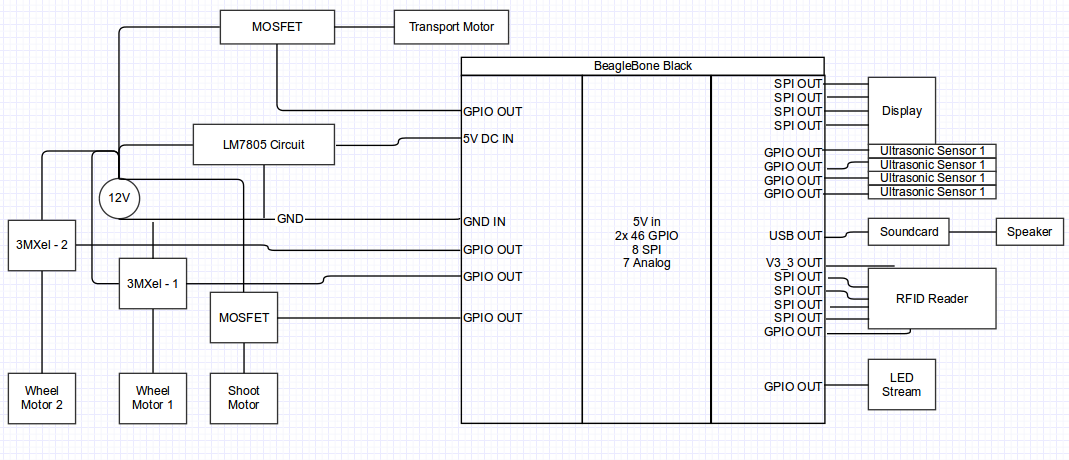
\includegraphics[width = 10cm]{Images/ElectronicalDiagram.png}
\caption{The circuit design}
\label{fig:electronics}
\end{center}
\end{figure}

\section{Part list}

\chapter{Planning Noverber to January}
Week 1 (10 November)\\
Ordering Parts\\
Building Parts\\
Programming\\
\\
Week 2 (17 November)\\
Building Parts\\
Programming\\
\\
Week 3 (24 November)\\
Assembling robot\\
	Mechanics\\
	Electronics
	Exterior design\\
	Programming\\
\\
Week 4 (1 December)
Assembling robot\\
Adjustments in prototype for safe test with user\\
\\
Week 5 (8 December)\\
Testing with user\\
\\
Week 6 (15 December)\\
Adjustments based on test with user\\
\\
Christmas break from the 22nd of December to 4th of January\\
\\
Week 7 (5 January)\\
Report\\
Prepare presentation\\
Poster\\
\\
Week 8 (12 January)\\
Report\\
Prepare presentation
Poster\\
\\
Week 9 (19 January) Tentamenweek\\
Week 10 (26 January) Tentamenweek

\chapter{Conclusion}
This report explained the design phase of this project. In the first phase of the design process several brainstorms were held. The first decision was to make a toy robot for a child. This would be an interesting branch to explore, since children find it fun to engage with a robot and this way it can be made fun to exercise or learn with a robot.
Next, a brainstorm was held to come up with ideas for the design and purpose of the robot. It was decided that the robot would be used to help children learn several subjects from school at home. Three concepts were chosen to be further improved, which would come to a final concept. After considering the three concepts, the turtle robot was chosen, since this robot was more unique and would be more interesting for the user. \\
The concept design is the next phase in the designing process. The turtle robot was further improved and all the parts were designed and chosen. A model was put together for the prototype from these parts, which was used to design the robot and to get a good idea of how the prototype would look. Furthermore all aspects of the robot were further improved and enhanced to make a base for the prototype. A name was chosen for the robot: Tawi. Use cases were designed for the use of the robot and improved for a more fluent interaction with the user. \\
\\
In the next part of this project the prototype of the robot will be build and tested.
\chapter{References}
Innvo Labs Corporation (2010), \textit{Pleoworld}, Retrieved 25 september 2014, \\from http://www.pleoworld.com/pleo\_rb/eng/index.php \\
\\
Spin Master (2014), \textit{Zoomer Pup}, Retrieved 25 september 2014, \\from http://www.zoomerpup.com/international/for\_parents.php?lang=nl\\
\\
Spin Master (2014), \textit{Zoomer Dino}, Retreived 25 september 2014, \\from http://www.zoomerdino.com/\#/home\\
\\
Anki (2014) \textit{Anki}, Retrieved 25 september 2014, \\from https://anki.com/en\#top \\
\\
LittleBits Electronics (2014) \textit{LittleBits}, Retrieved 25 september 2014,\\ from http://littlebits.cc/ \\
\\
Ubooly Inc. (2014), \textit{Ubooly}, Retrieved 25 september 2014,\\ from http://www.ubooly.com/ \\
\\
Kickstarter Inc. (2014) \textit{Kickstarter}, Retrieved 25 september 2014, \\from https://www.kickstarter.com/ \\
\\
Hasbro (2014) \textit{Hasbro}, Retrieved 25 september 2014, \\from http://www.hasbro.com/nl\_NL/ \\
\\
Hasbro (2014) \textit{Furby}, Retrieved 25 september 2014, \\from http://www.hasbro.com/furby/nl\_NL/ \\
\\
Sphere (2014), \textit{GoSphero}, Retrieved 25 september 2014,\\ from http://www.gosphero.com/ \\
\\
Gray, L.(2014), Britain’s ‘\textit{litter epidemic’ costs almost £1bn every year}’ , Retrieved 15 October 2014, \\from http://www.telegraph.co.uk/earth/earthnews/7897112/Britains-litter-epidemic-costs-almost-1bn-every-year.html \\
\\
Viola, N., Corpino, S., Fioriti, M. and Stesina. F.(2012) \textit{Functional Analysis in Systems Engineering: Methodology and Applications}, Retrieved 10 September 2014, \\from http://cdn.intechopen.com/pdfs-wm/32617\.pdf \\
\\
Choosing Safe Toys, (n.d.), Retrieved 29 September 2014, \\from http://kidshealth.org/parent/firstaid\_safe/home/safe\_toys.html \\
\\
Engineering \lq\lq{}Laws\rq\rq{} - Moore\rq{}s, Rock\rq{}s, Butter\rq{}s and others (2012), Retrieved 22 October 2014, \\from http://sourcetech411.com/2012/12/engineering-laws-moores-rocks-butters-and-others/ \\
\\
DYKA (2003), \textit{Technicshe Documentatie drukleiding PVC}, Retrieved 23 October 2014 \\
from http://www.dyka.nl/nl/binaries/2010\%20TD\%20Drukleiding\%20PVC\%20en\%20PE\%20maart\%202003\%20nwe\%20omslag\_tcm29-6927.pdf \\
\\
Battery Discharge Methods, (n.d.), Retrieved 23 October 2014, \\from http://batteryuniversity.com/learn/article/discharge\_methods\\
\\
Lead Based Batteries, (n.d.), Retrieved 23 October 2014, \\from http://batteryuniversity.com/learn/article/lead\_based\_batteries \\
\\
Lithium Based Batteries, (n.d.), Retrieved 23 October 2014, \\from http://batteryuniversity.com/learn/article/lithium\_based\_batteries \\
\\
Nickel Based Batteries, (n.d.), Retrieved 23 October 2014, \\from 
http://batteryuniversity.com/learn/article/nickel\_based\_batteries \\
\\
Nintendo (2014) Torkoal, Retrieved on 29 september 2014\\ from http://www.pokemon.com/nl/pokedex/torkoal \\
\\
Child development: 6-9 years, (n.d.), Retrieved 24 October 2014, \\from http://www.cyh.com/HealthTopics/HealthTopicDetails.aspx?p=114\&np=122\&id=1867\\
\\
\begin{appendices}
\chapter{Use Case}
\label{appendix:usecase}
\chapter{MoSCoW model}
\label{appendix:moscow}
\section{Musts}
\section{Shoulds}
\section{Coulds}
\section{won'ts}
\chapter{Brainstorm initial designs}
\label{appendix:brainstorm}
\chapter{Different games}
\label{appendix:games}
\chapter{Details software design}
\label{appendix:software}
\chapter{Competitors}
\label{appendix:competitors}
\section{Innvo Labs}
\section{Zoomer}
\section{Orbotix}
\section{Anki}
\section{LittleBits Electronics}
\section{Ubooly Inc.}
\section{Hasbro}
\chapter{Battery}
\begin{table}[h]
\caption{Battery options}
\begin{tabular}{llllll}
  & Voltage  & Capacity & Type  & Price per piece & Price for requirements          \\
         & (V)      & (mAh) &                 &                        &         \\
Option 1 & 3.7      & 4400  & Li-Ion          & \$19.90                & \$59.70 \\
Option 2 & 11.1     & 2200  & Li-Ion          & \$26.99                & \$53.98 \\
Option 3 & 12       & 9500  & NiMH            & \$84.15                & \$84.15 \\
Option 4 & 12       & 3700  & NiMH            & \$44.99                & \$44.99
\end{tabular}
\label{table:batteryOptions}
\end{table}

\begin{sidewaystable}
\caption{Battery requirements}
\begin{center}
\begin{tabular}{m{2cm}|m{2cm}|m{2cm}|m{2cm}|m{2cm}|m{2cm}|m{2cm}|m{3.2cm}|}
Name               & Current & Time type      & Maximum Capacity 30 min & Effective Required Capacity & Minimum Capacity 30 min & Effective Required Capacity & Average Effective Required Capacity \\
                   & (A)     &                & (Ah)                    & (Ah)                        & (Ah)                    & (Ah)                        & (Ah)                                \\
Shooting Motor     & 4       & While Shooting & 2                       & 2.8571                & 0                       & 0                           & 1.4285                        \\
Wheel motors       & 1       & While Driving  & 0.5                     & 0.7142               & 0                       & 0                           & 0.3571                        \\
RFID Reader        & 0.01    & Full Time      & 0.005                   & 0.0071                & 0.005                   & 0.0071                & 0.00714 \\
Ultrasonic Sensors & 0.06    & Full Time      & 0.03                    & 0.0428              & 0.03                    & 0.0428                & 0.0428                        \\
LEDs               & 0.6     & Full Time      & 0.3                     & 0.4285                & 0.3                     & 0.4285                & 0.4285                       \\
BeagleBone         & 0.46    & Full Time      & 0.23                    & 0.3285               & 0.23                    & 0.3285               & 0.3285                        \\
Display            & 0.04    & Full Time      & 0.02                    & 0.0285                & 0.02                    & 0.0286               & 0.0285                        \\
Sound              & 0.002   & While Speaking & 0.001                   & 0.0014              & 0                       & 0                           & 0.0007                        \\
Total              & 6.172   &     -           & 3.086                   & 4.4085               & 0.585                   & 0.8357               & 2.6221                       
\end{tabular}
\end{center}
\label{table:battery}
\end{sidewaystable}
\label{appendix:battery}
\chapter{Drawings}
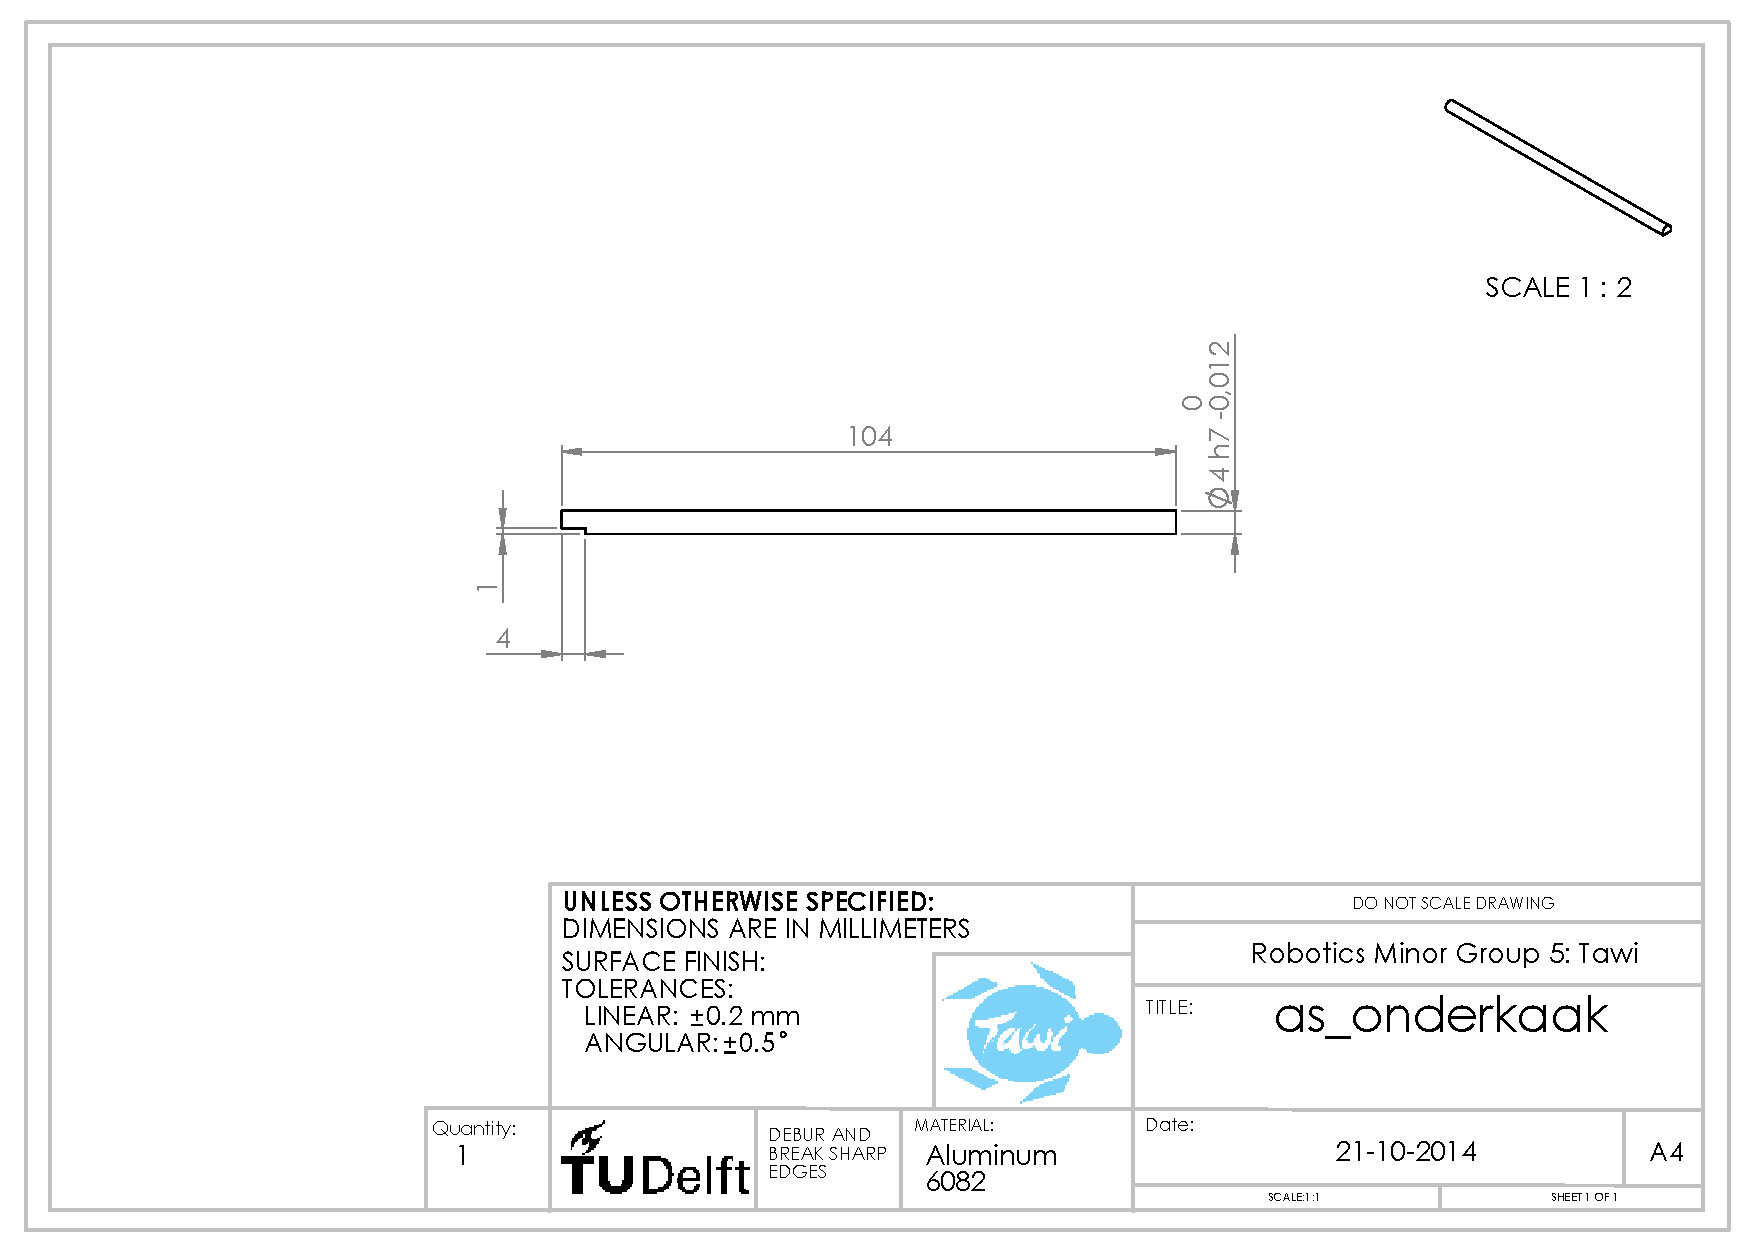
\includepdf[pages={1},landscape=true]{pdfdrawings/as_onderkaak.PDF}
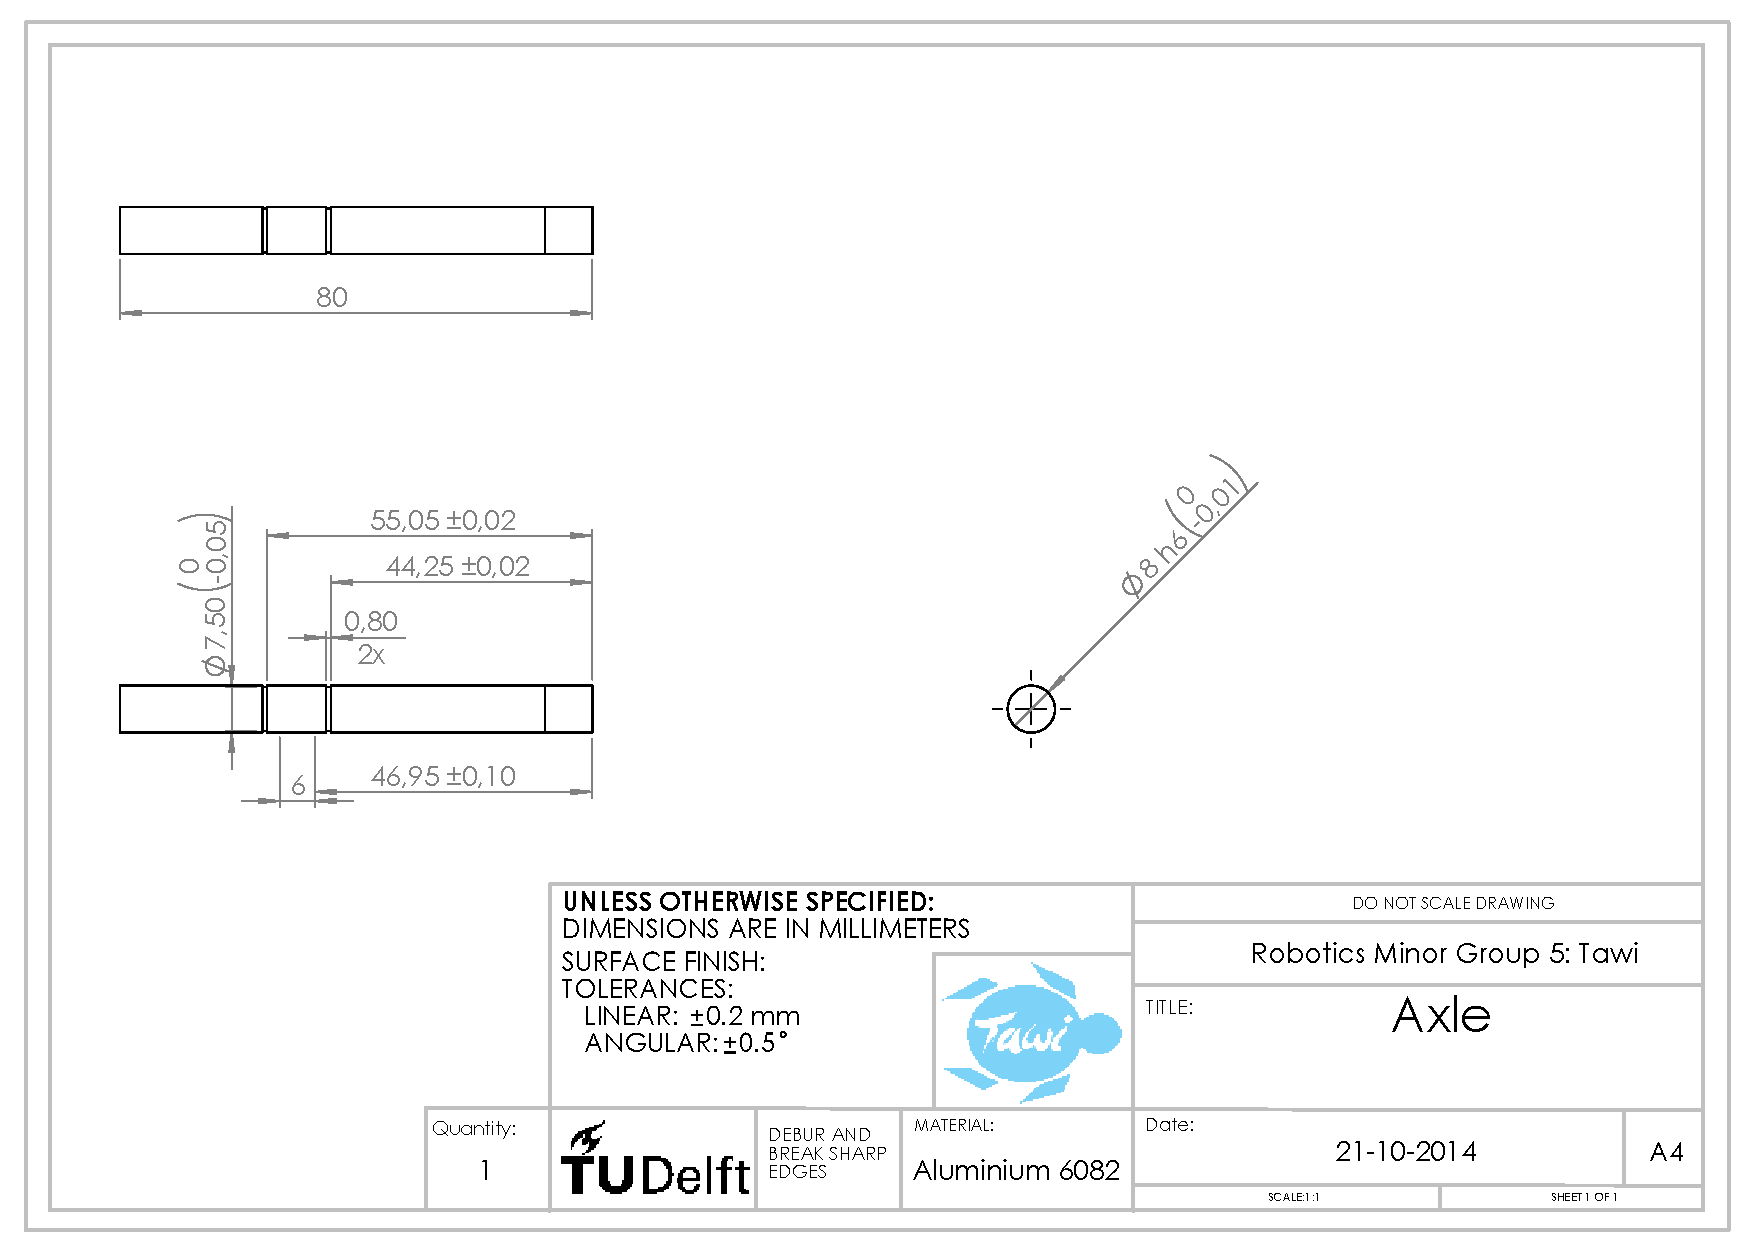
\includepdf[pages={1},landscape=true]{pdfdrawings/Axle.PDF}
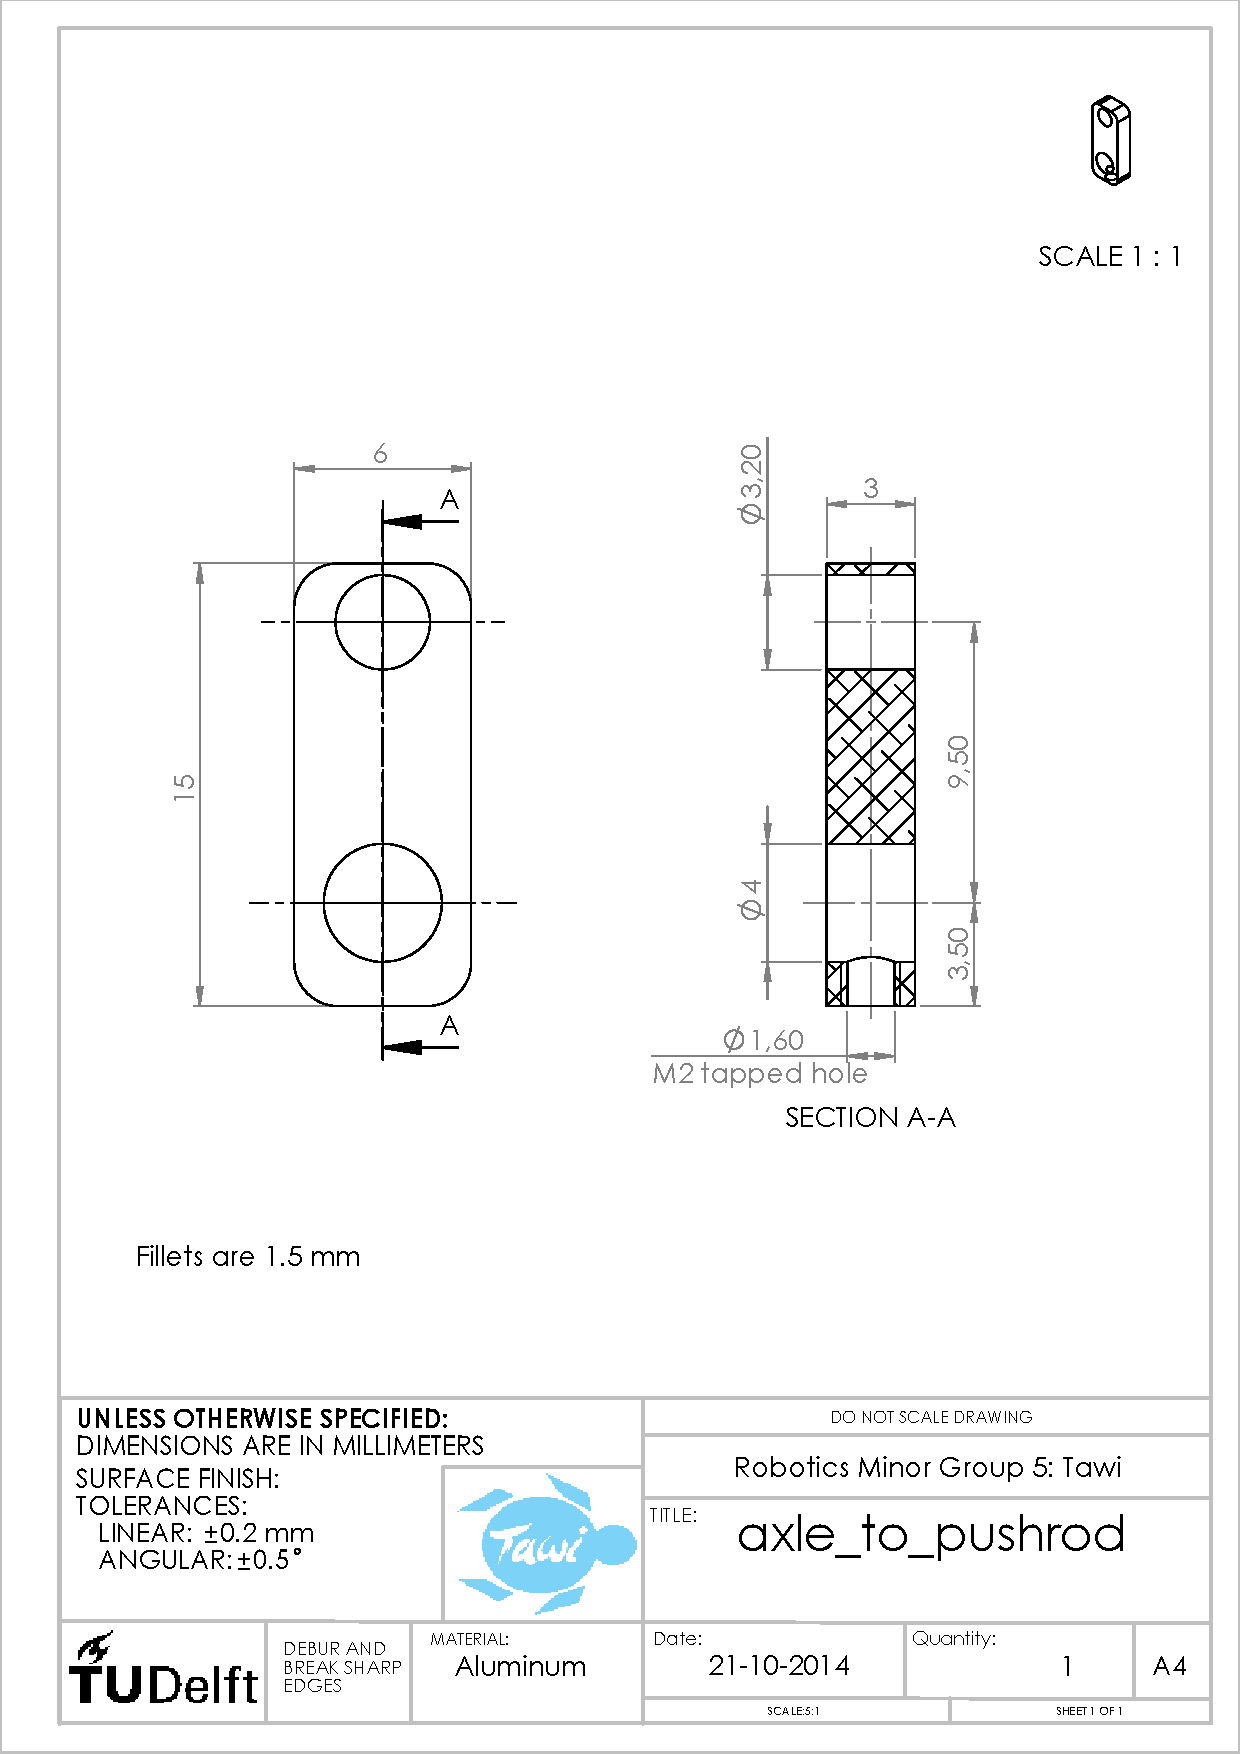
\includepdf[pages={1}]{pdfdrawings/axle_to_pushrod.PDF}
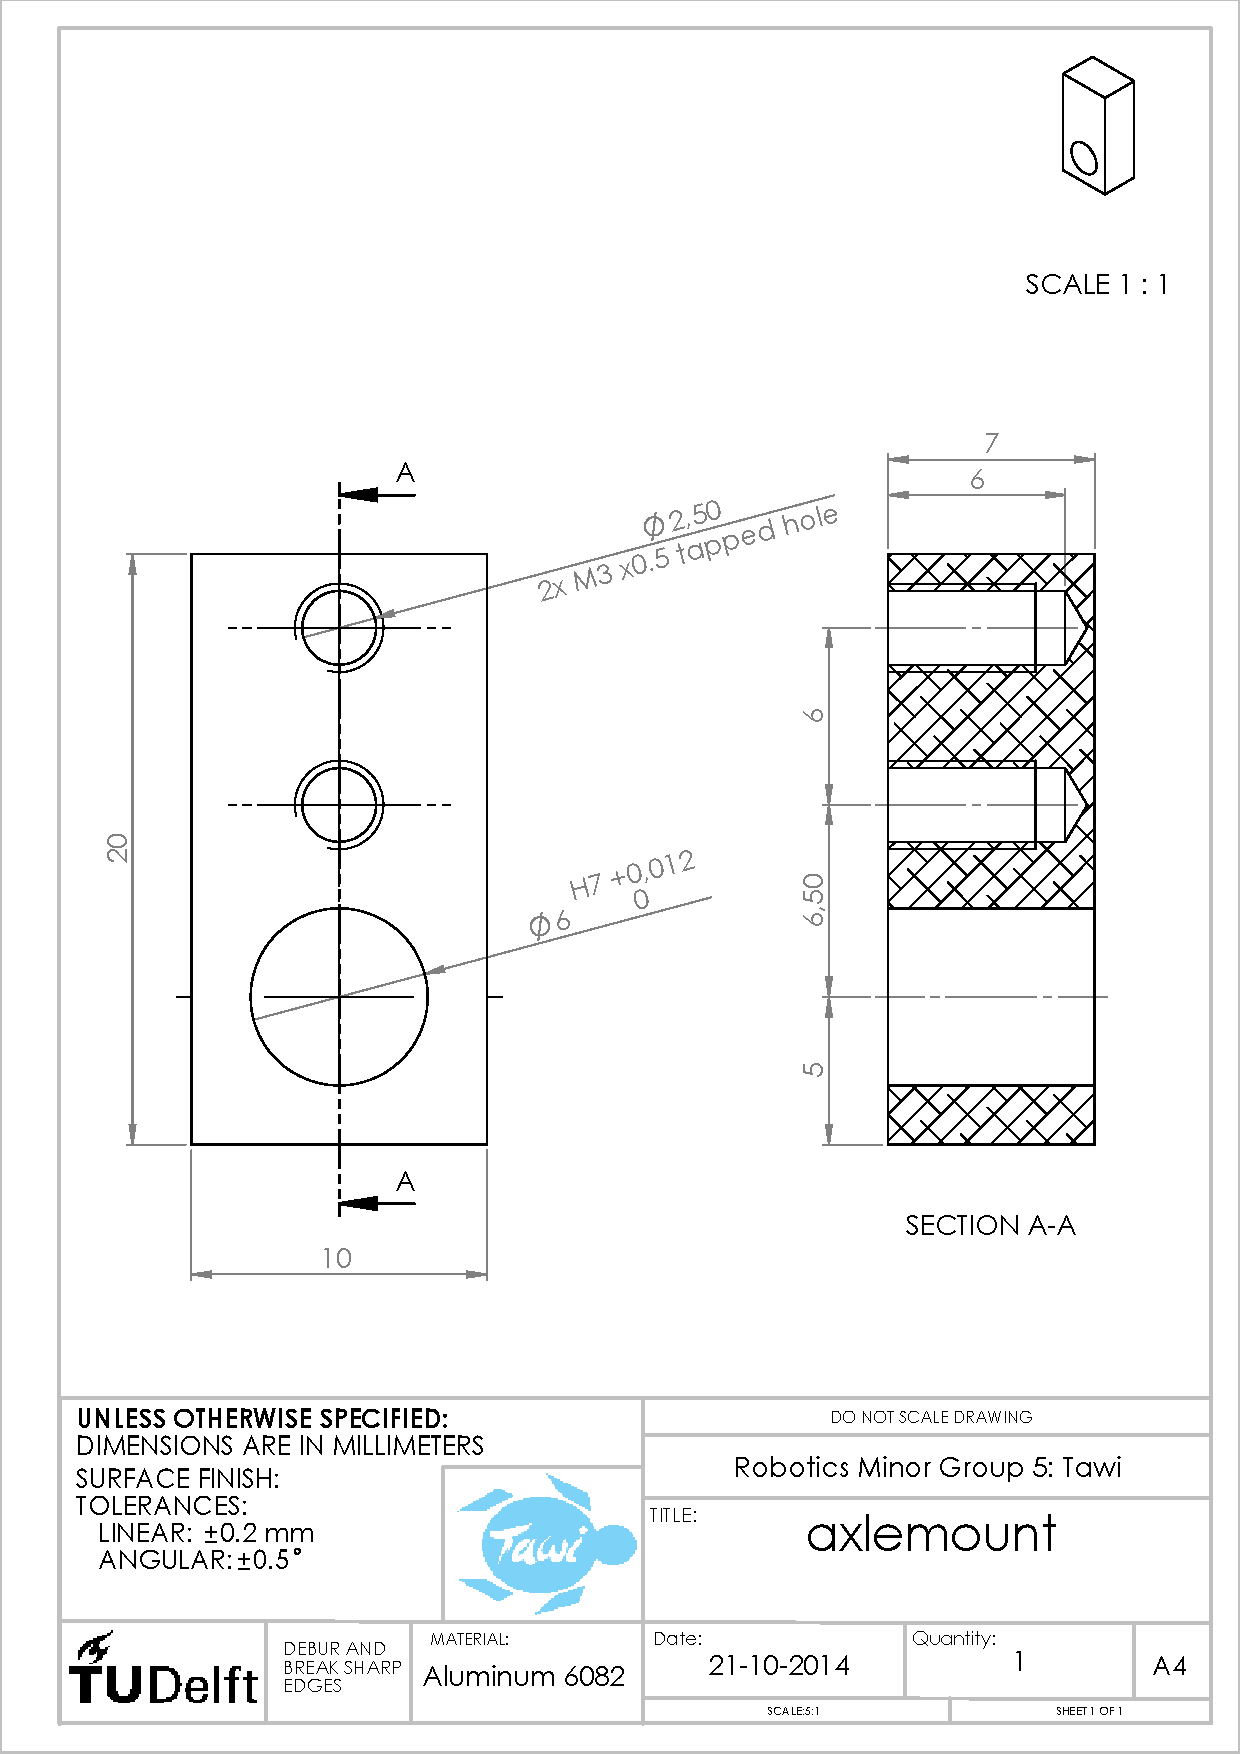
\includepdf[pages={1}]{pdfdrawings/axlemount.PDF}
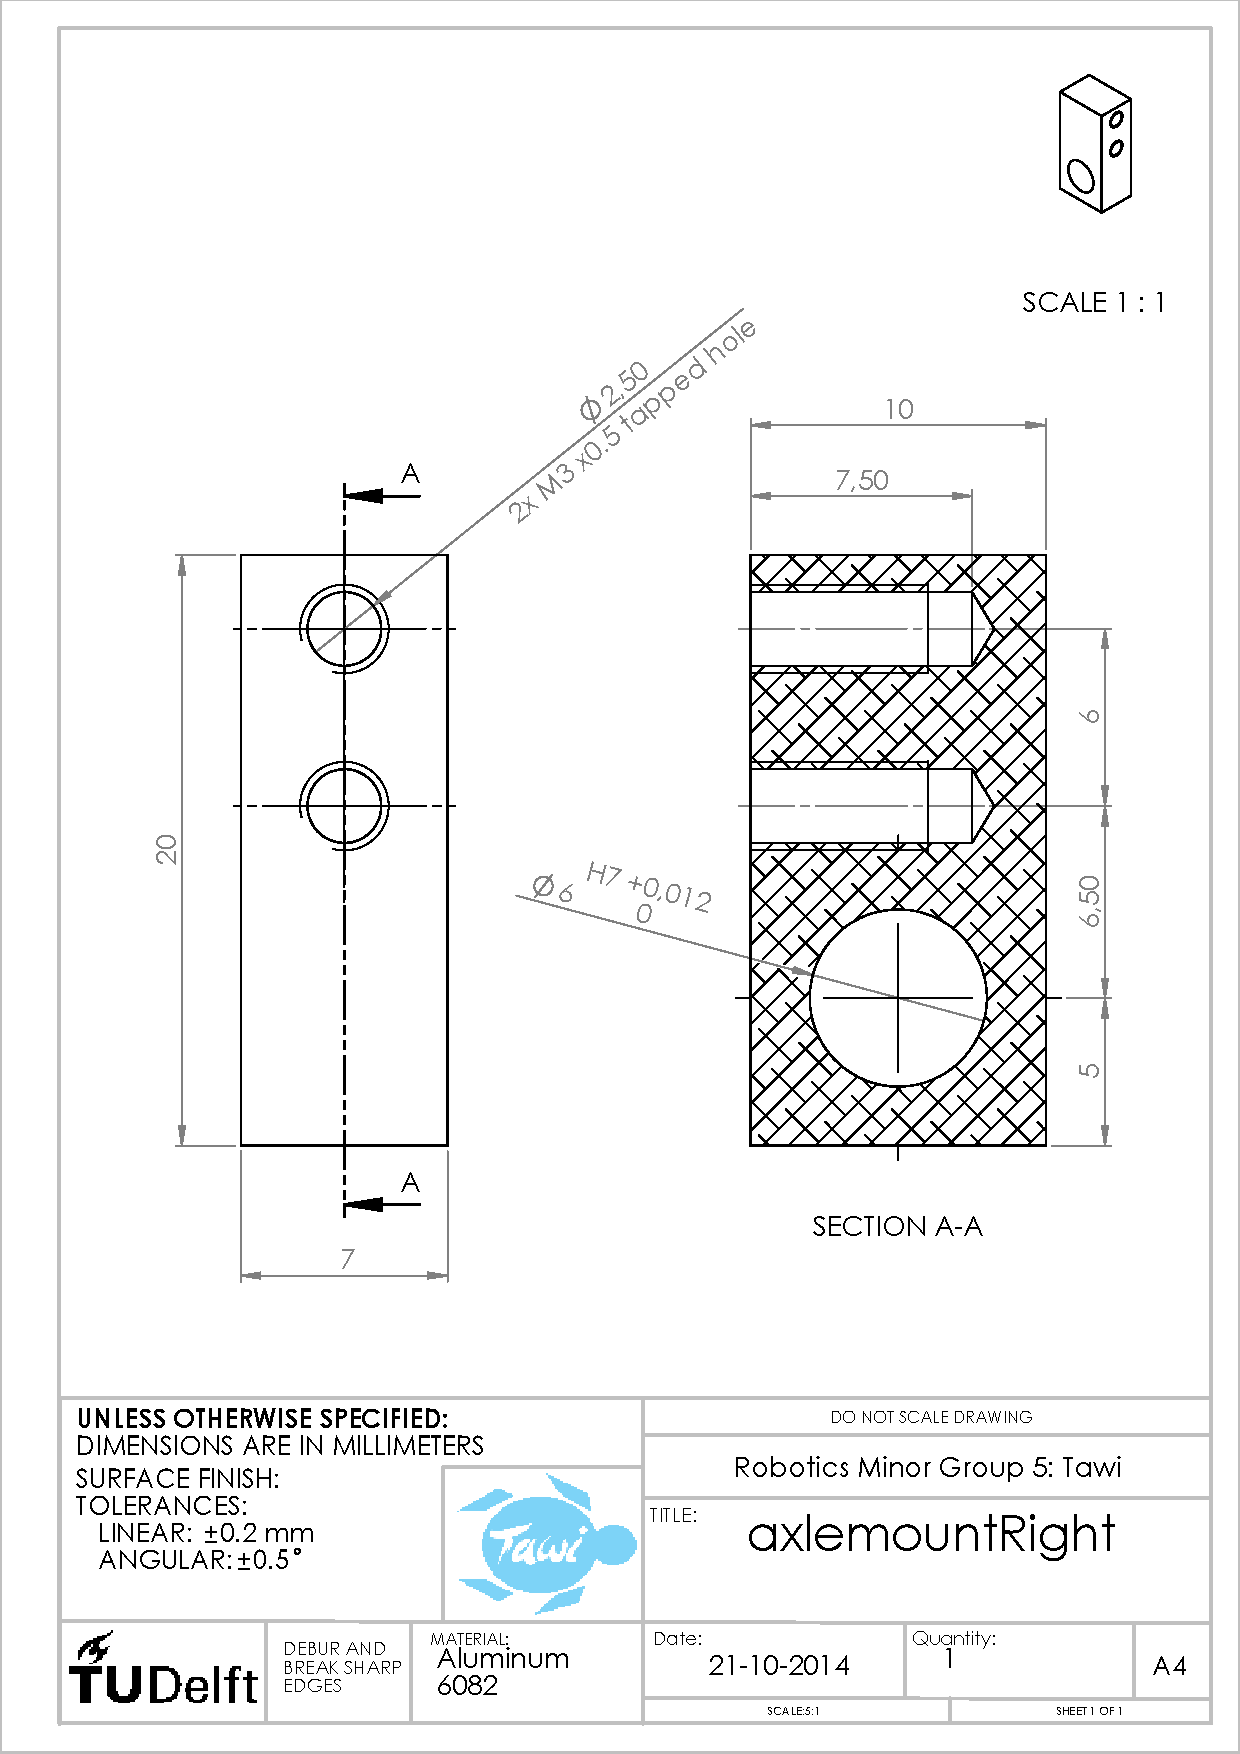
\includepdf[pages={1}]{pdfdrawings/axlemountRight.PDF}
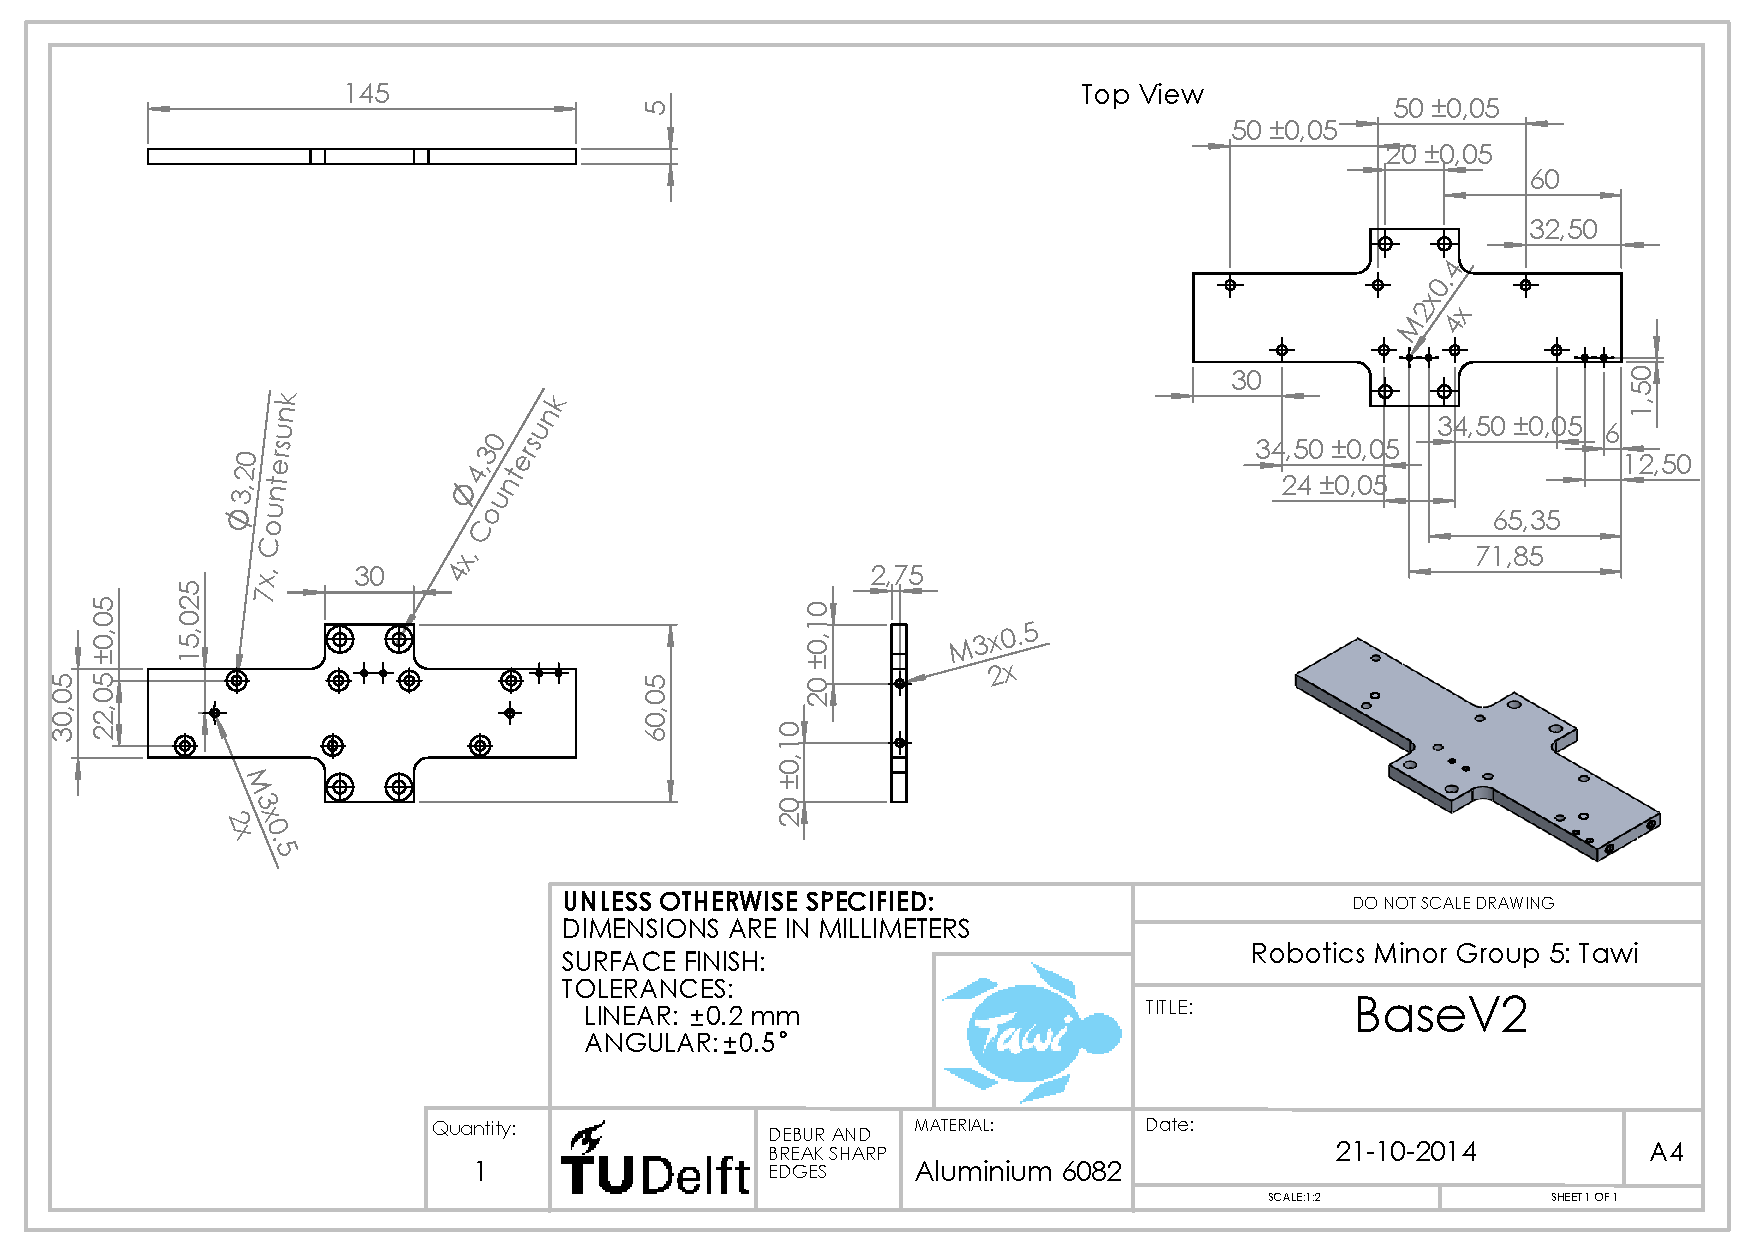
\includepdf[pages={1},landscape=true]{pdfdrawings/BaseV2.PDF}
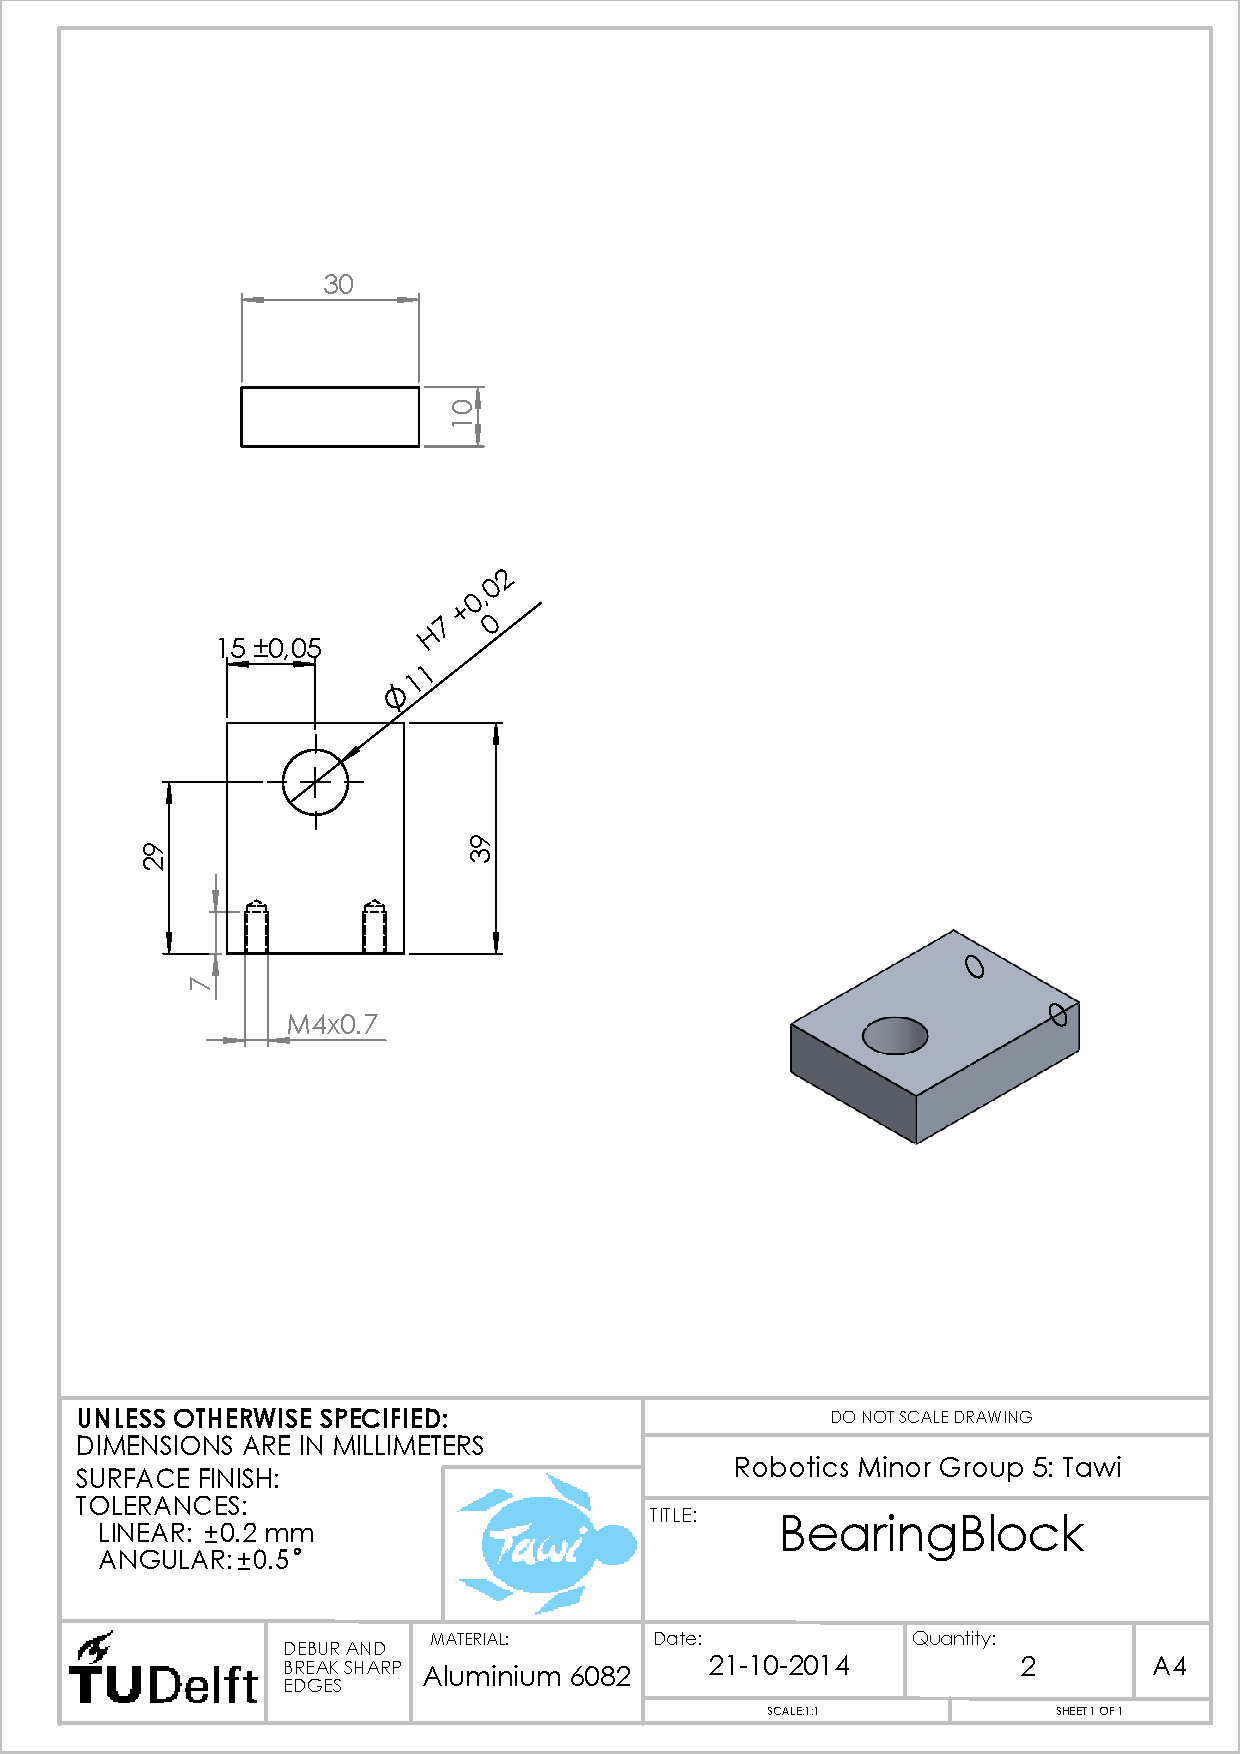
\includepdf[pages={1}]{pdfdrawings/BearingBlock.PDF}
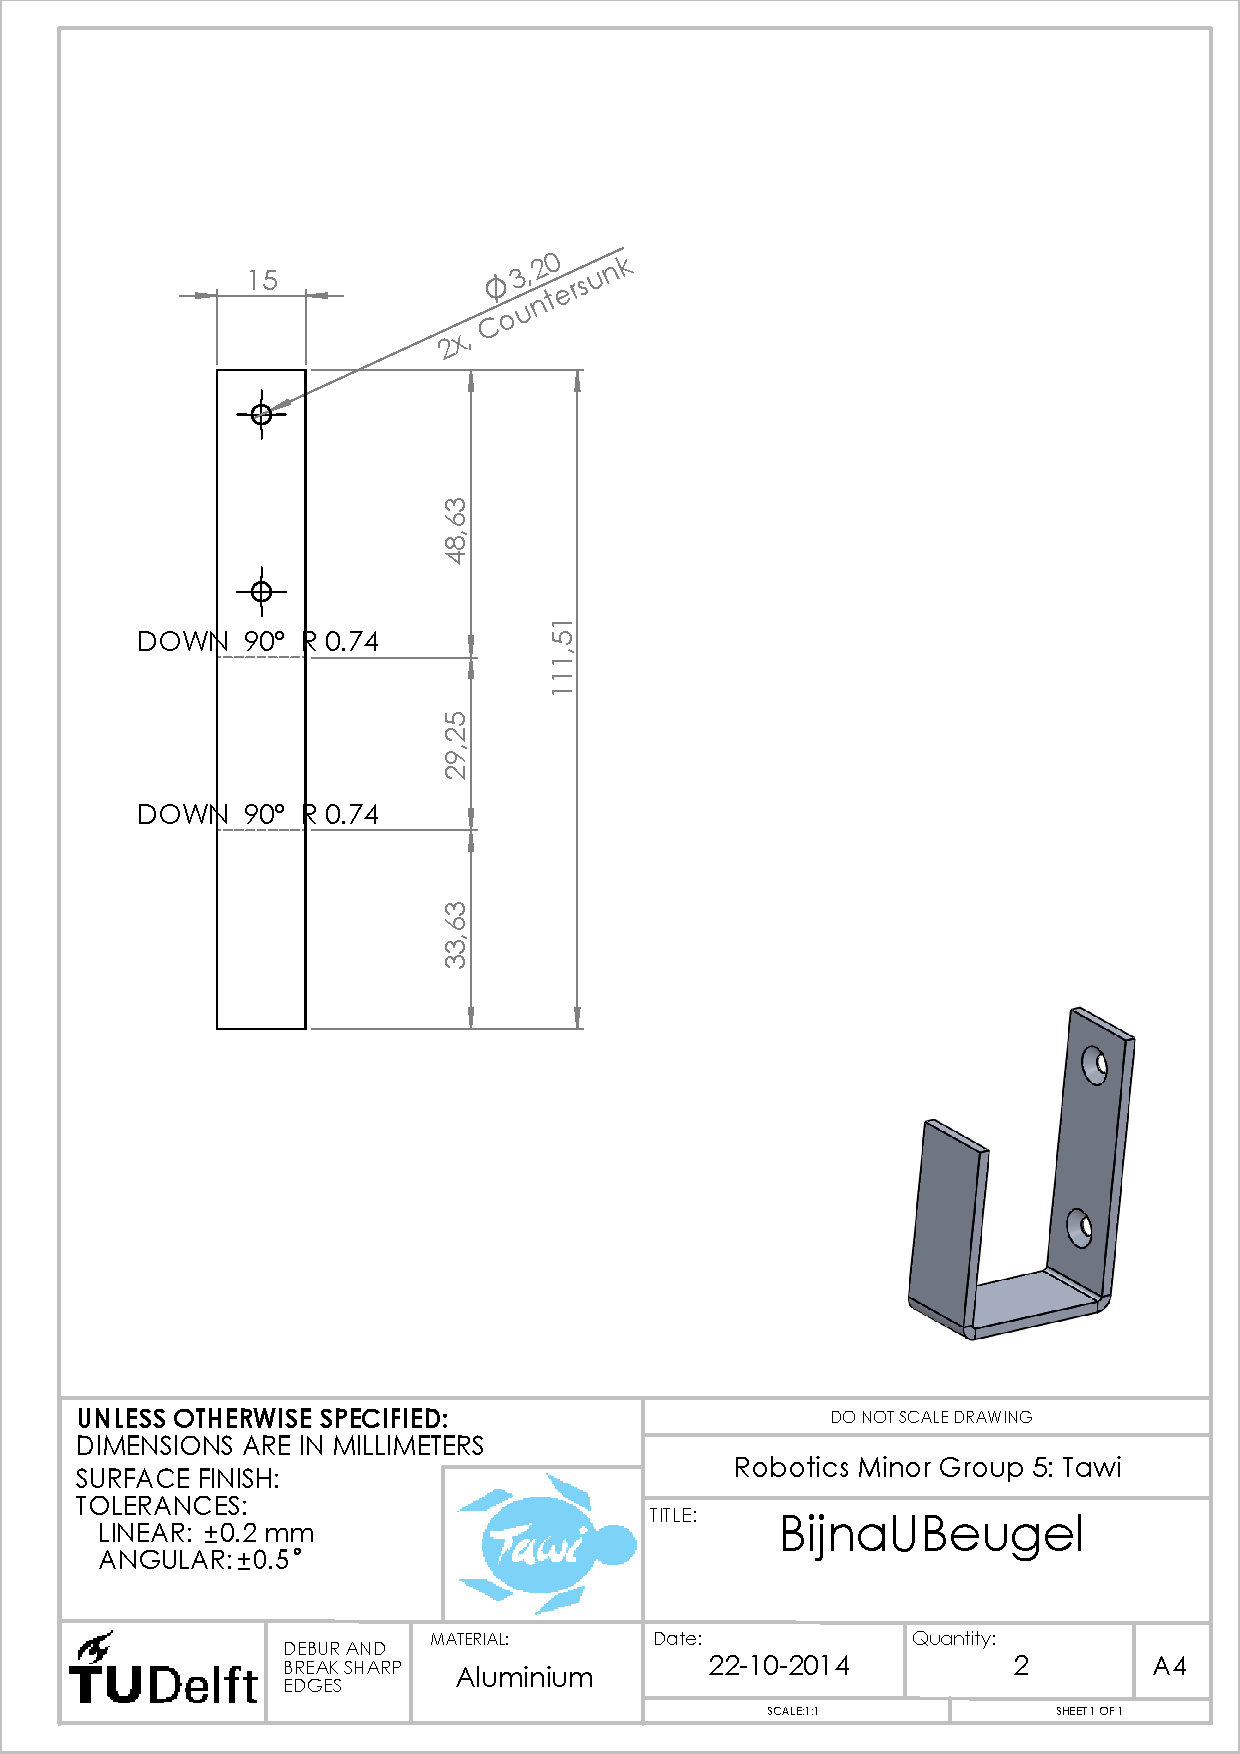
\includepdf[pages={1}]{pdfdrawings/BijnaUBeugel.PDF}
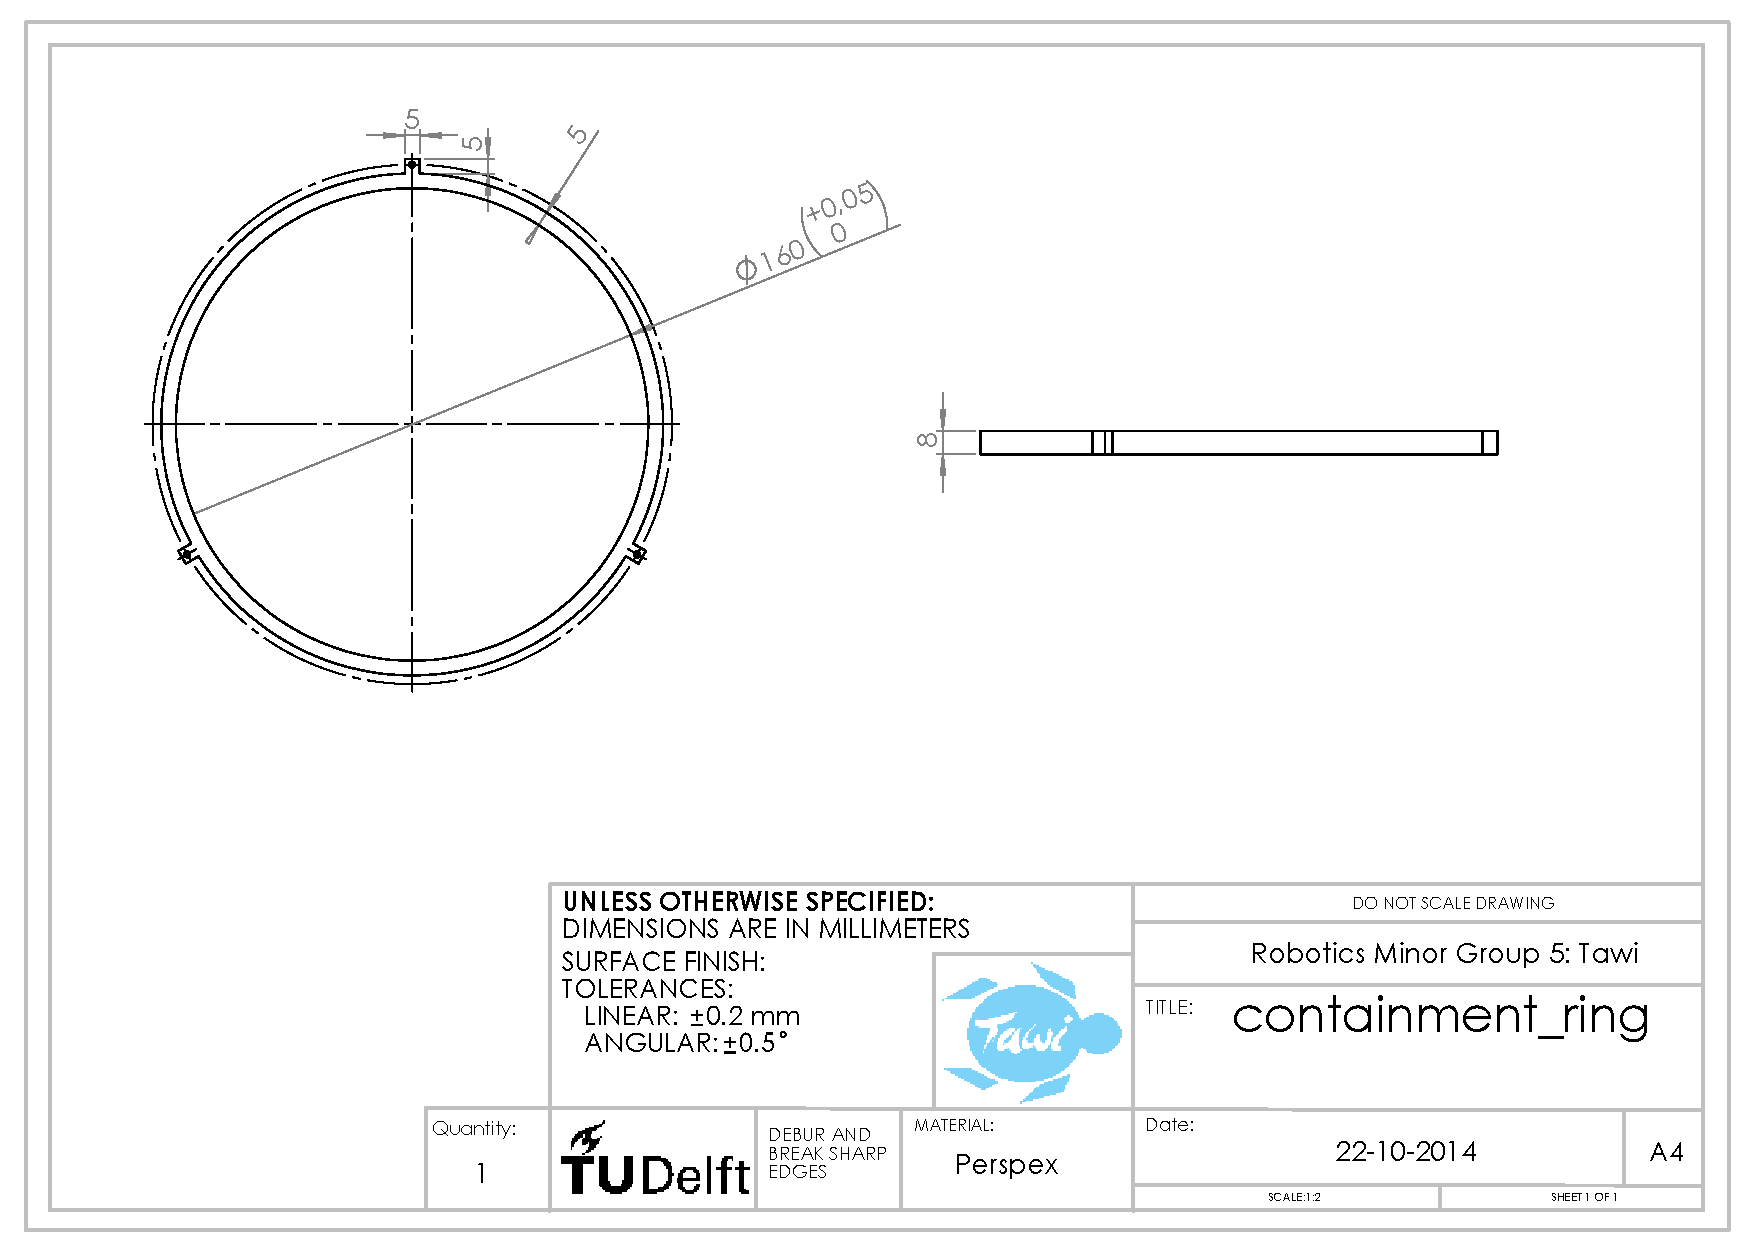
\includepdf[pages={1},landscape=true]{pdfdrawings/containment_ring.PDF}
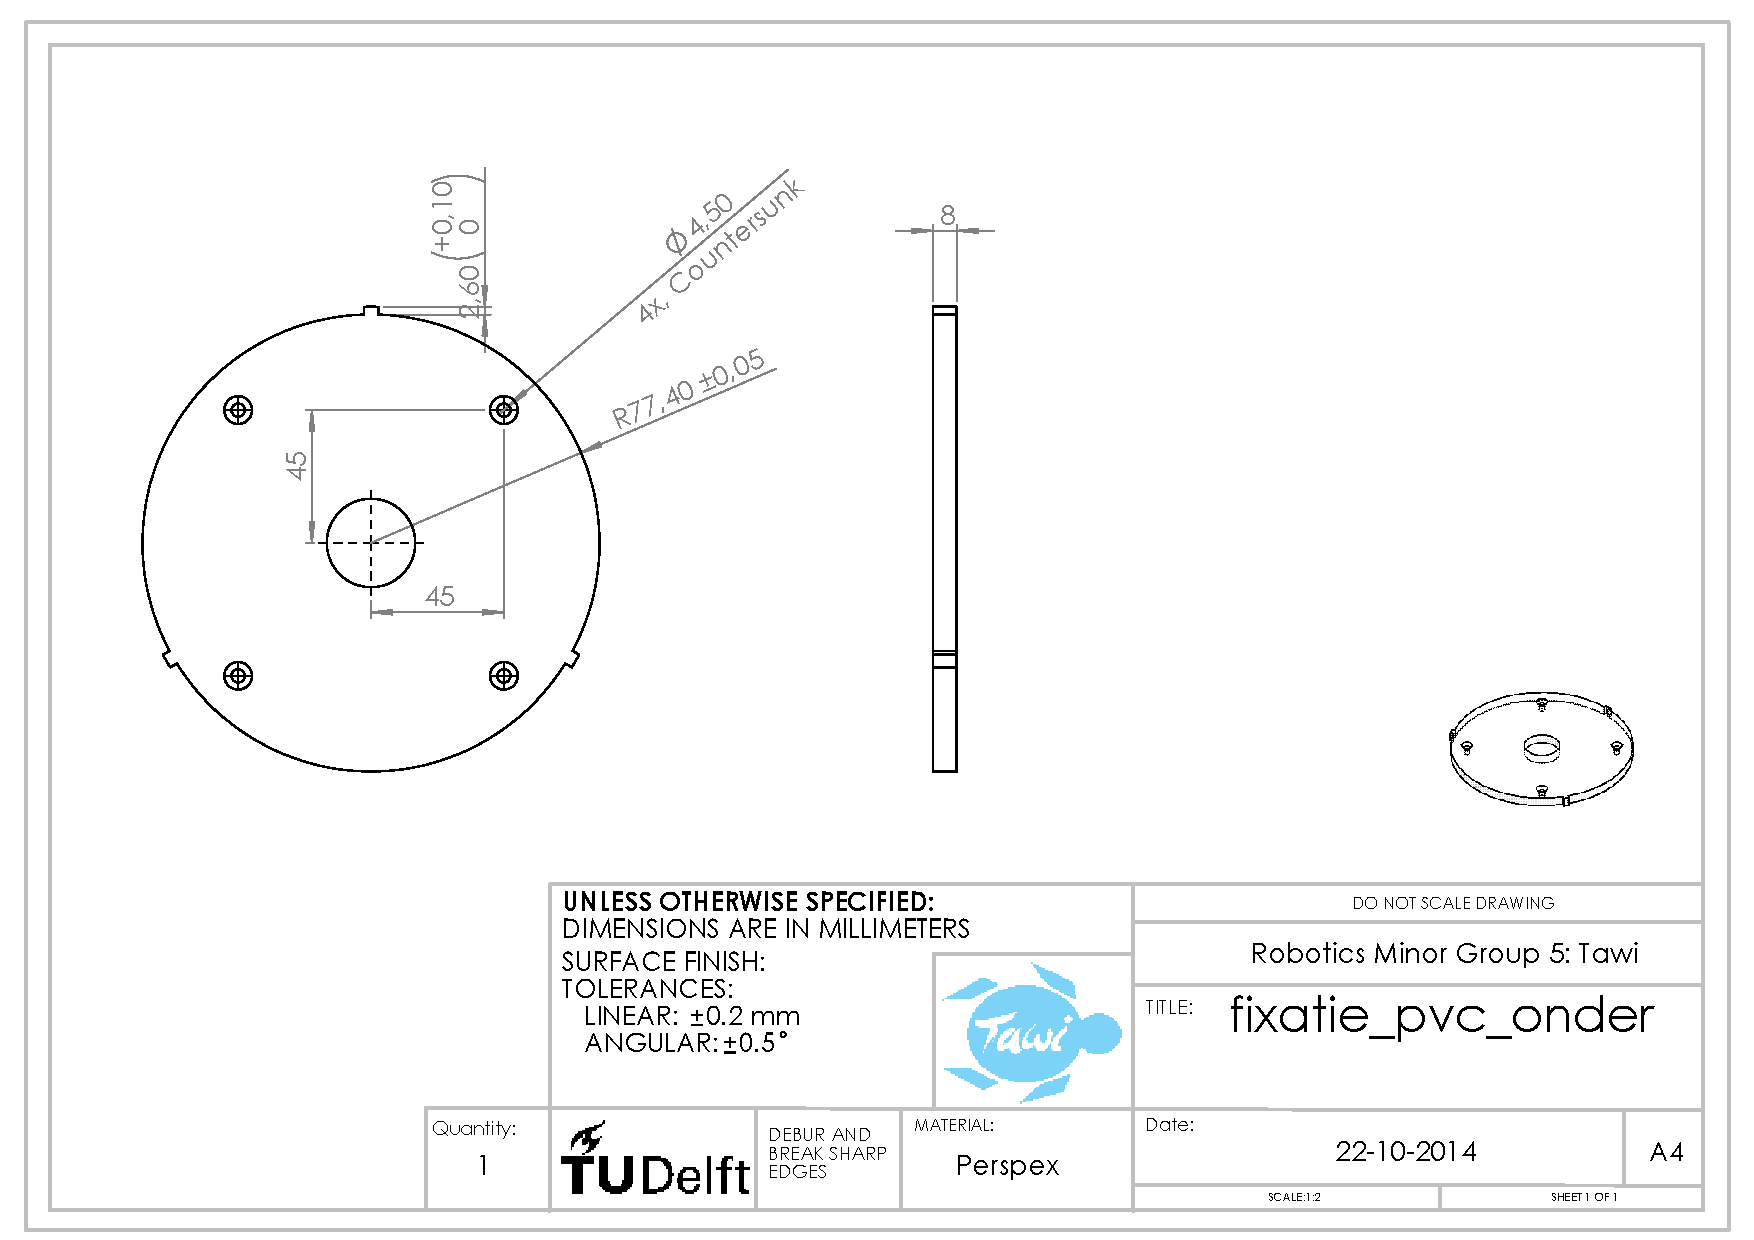
\includepdf[pages={1},landscape=true]{pdfdrawings/fixatie_pvc_onder.PDF}
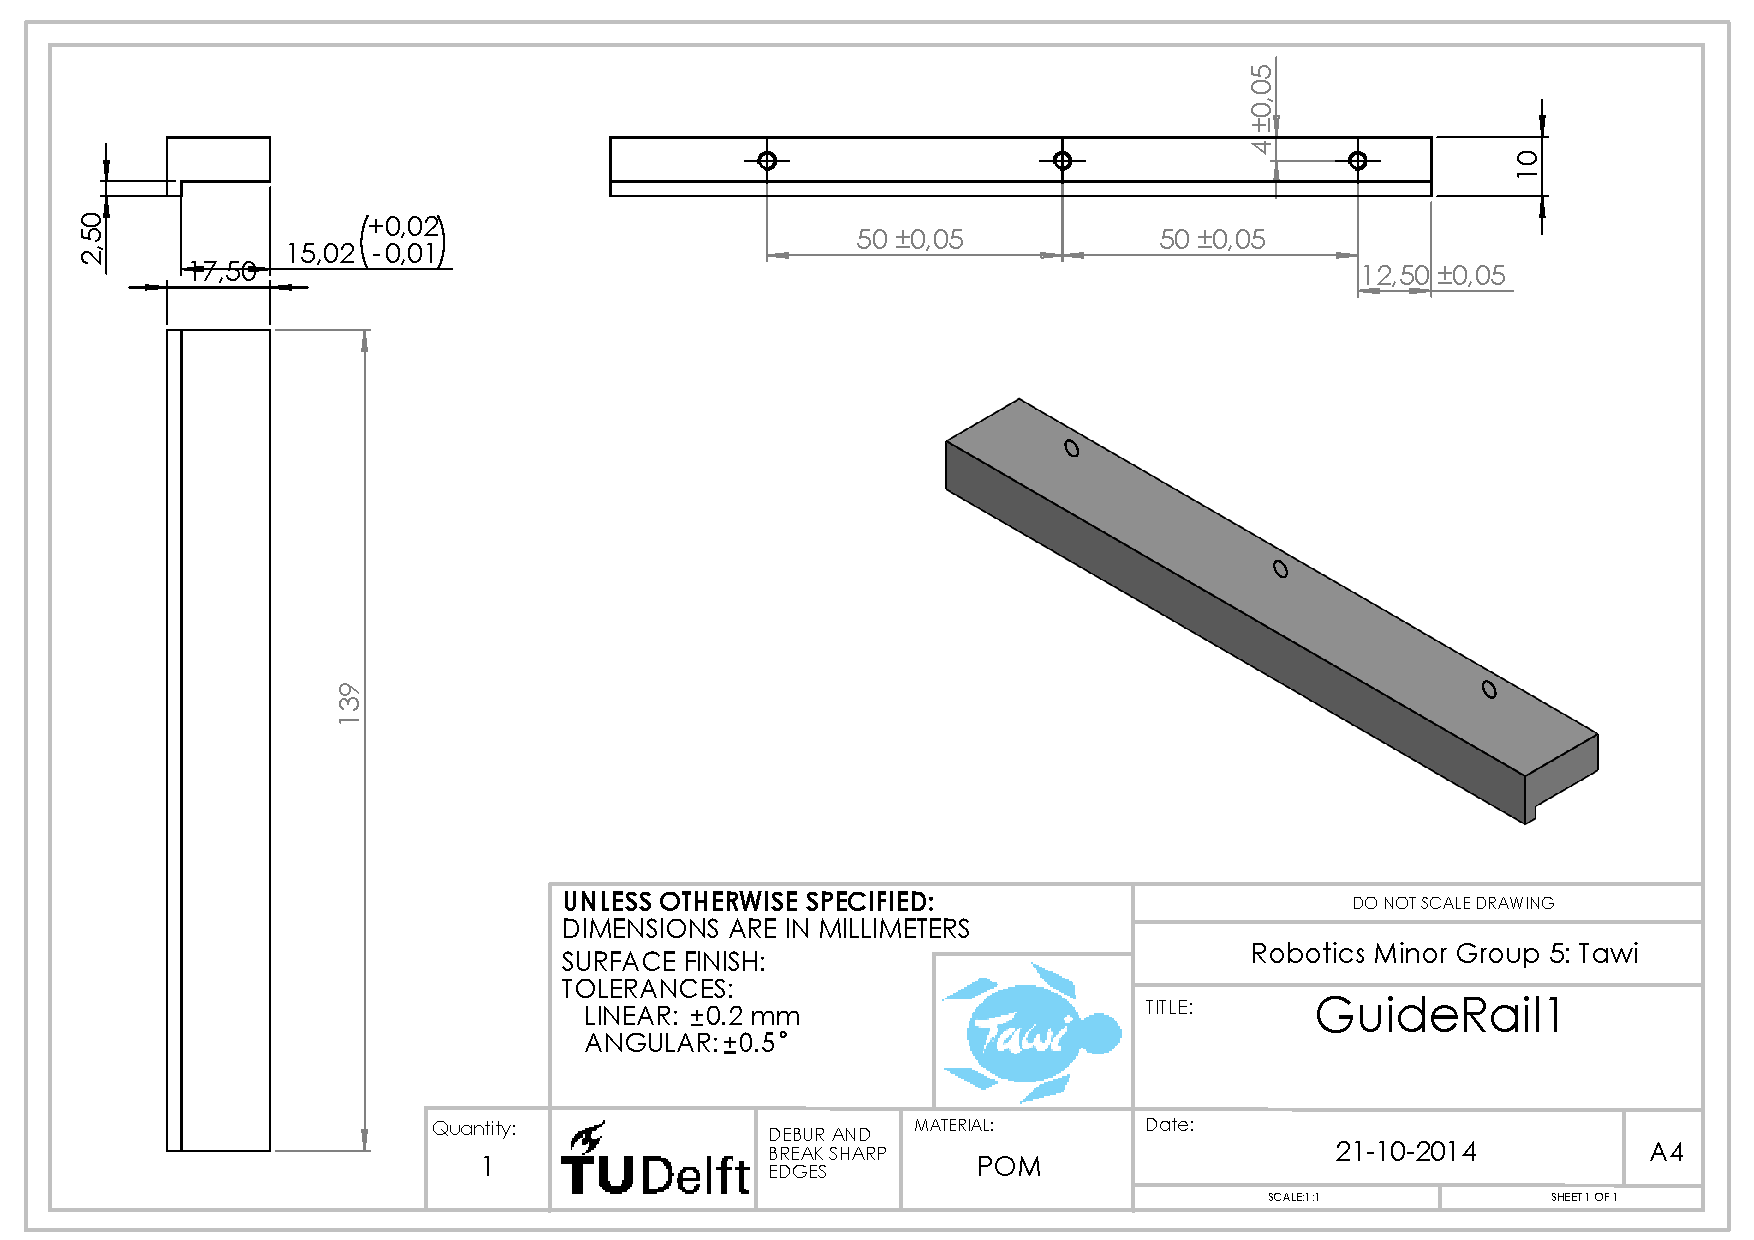
\includepdf[pages={1},landscape=true]{pdfdrawings/GuideRail1.PDF}
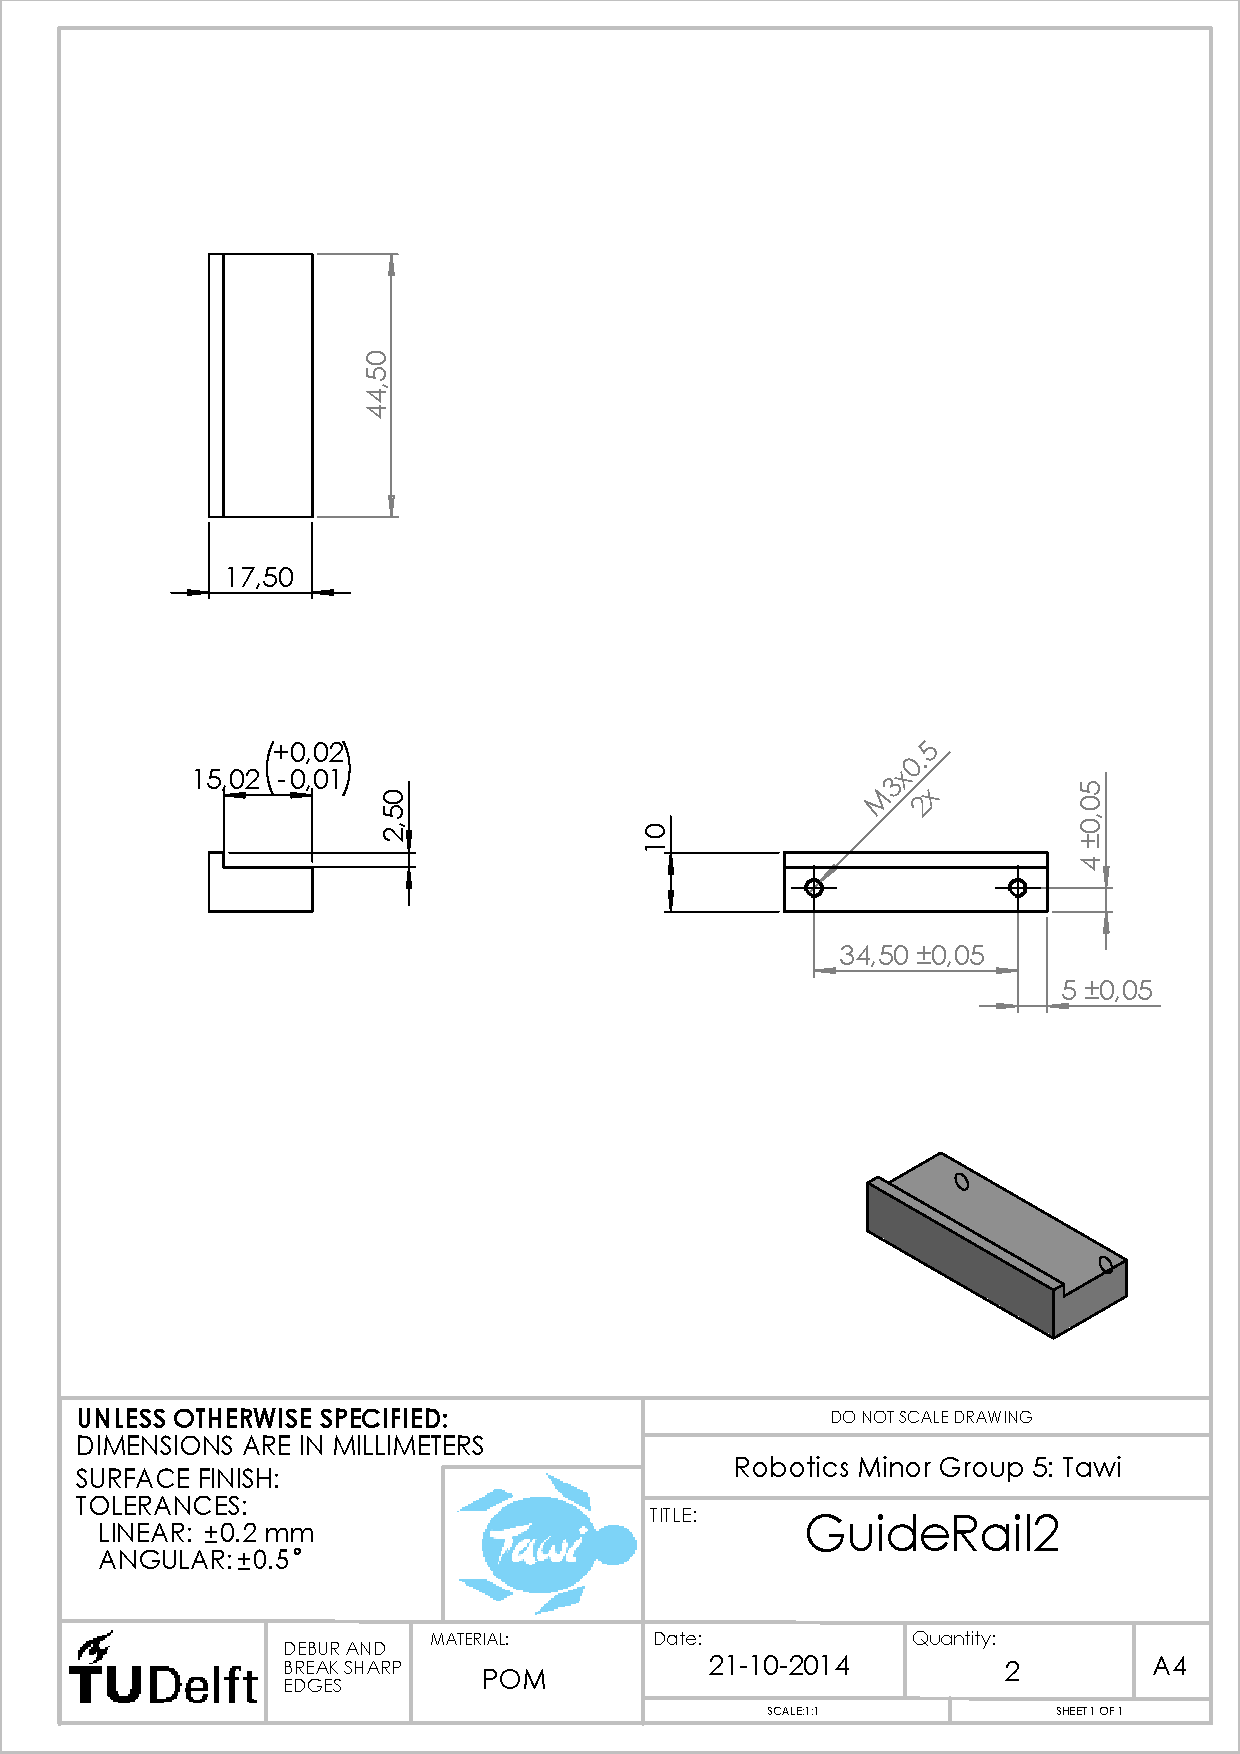
\includepdf[pages={1}]{pdfdrawings/GuideRail2.PDF}
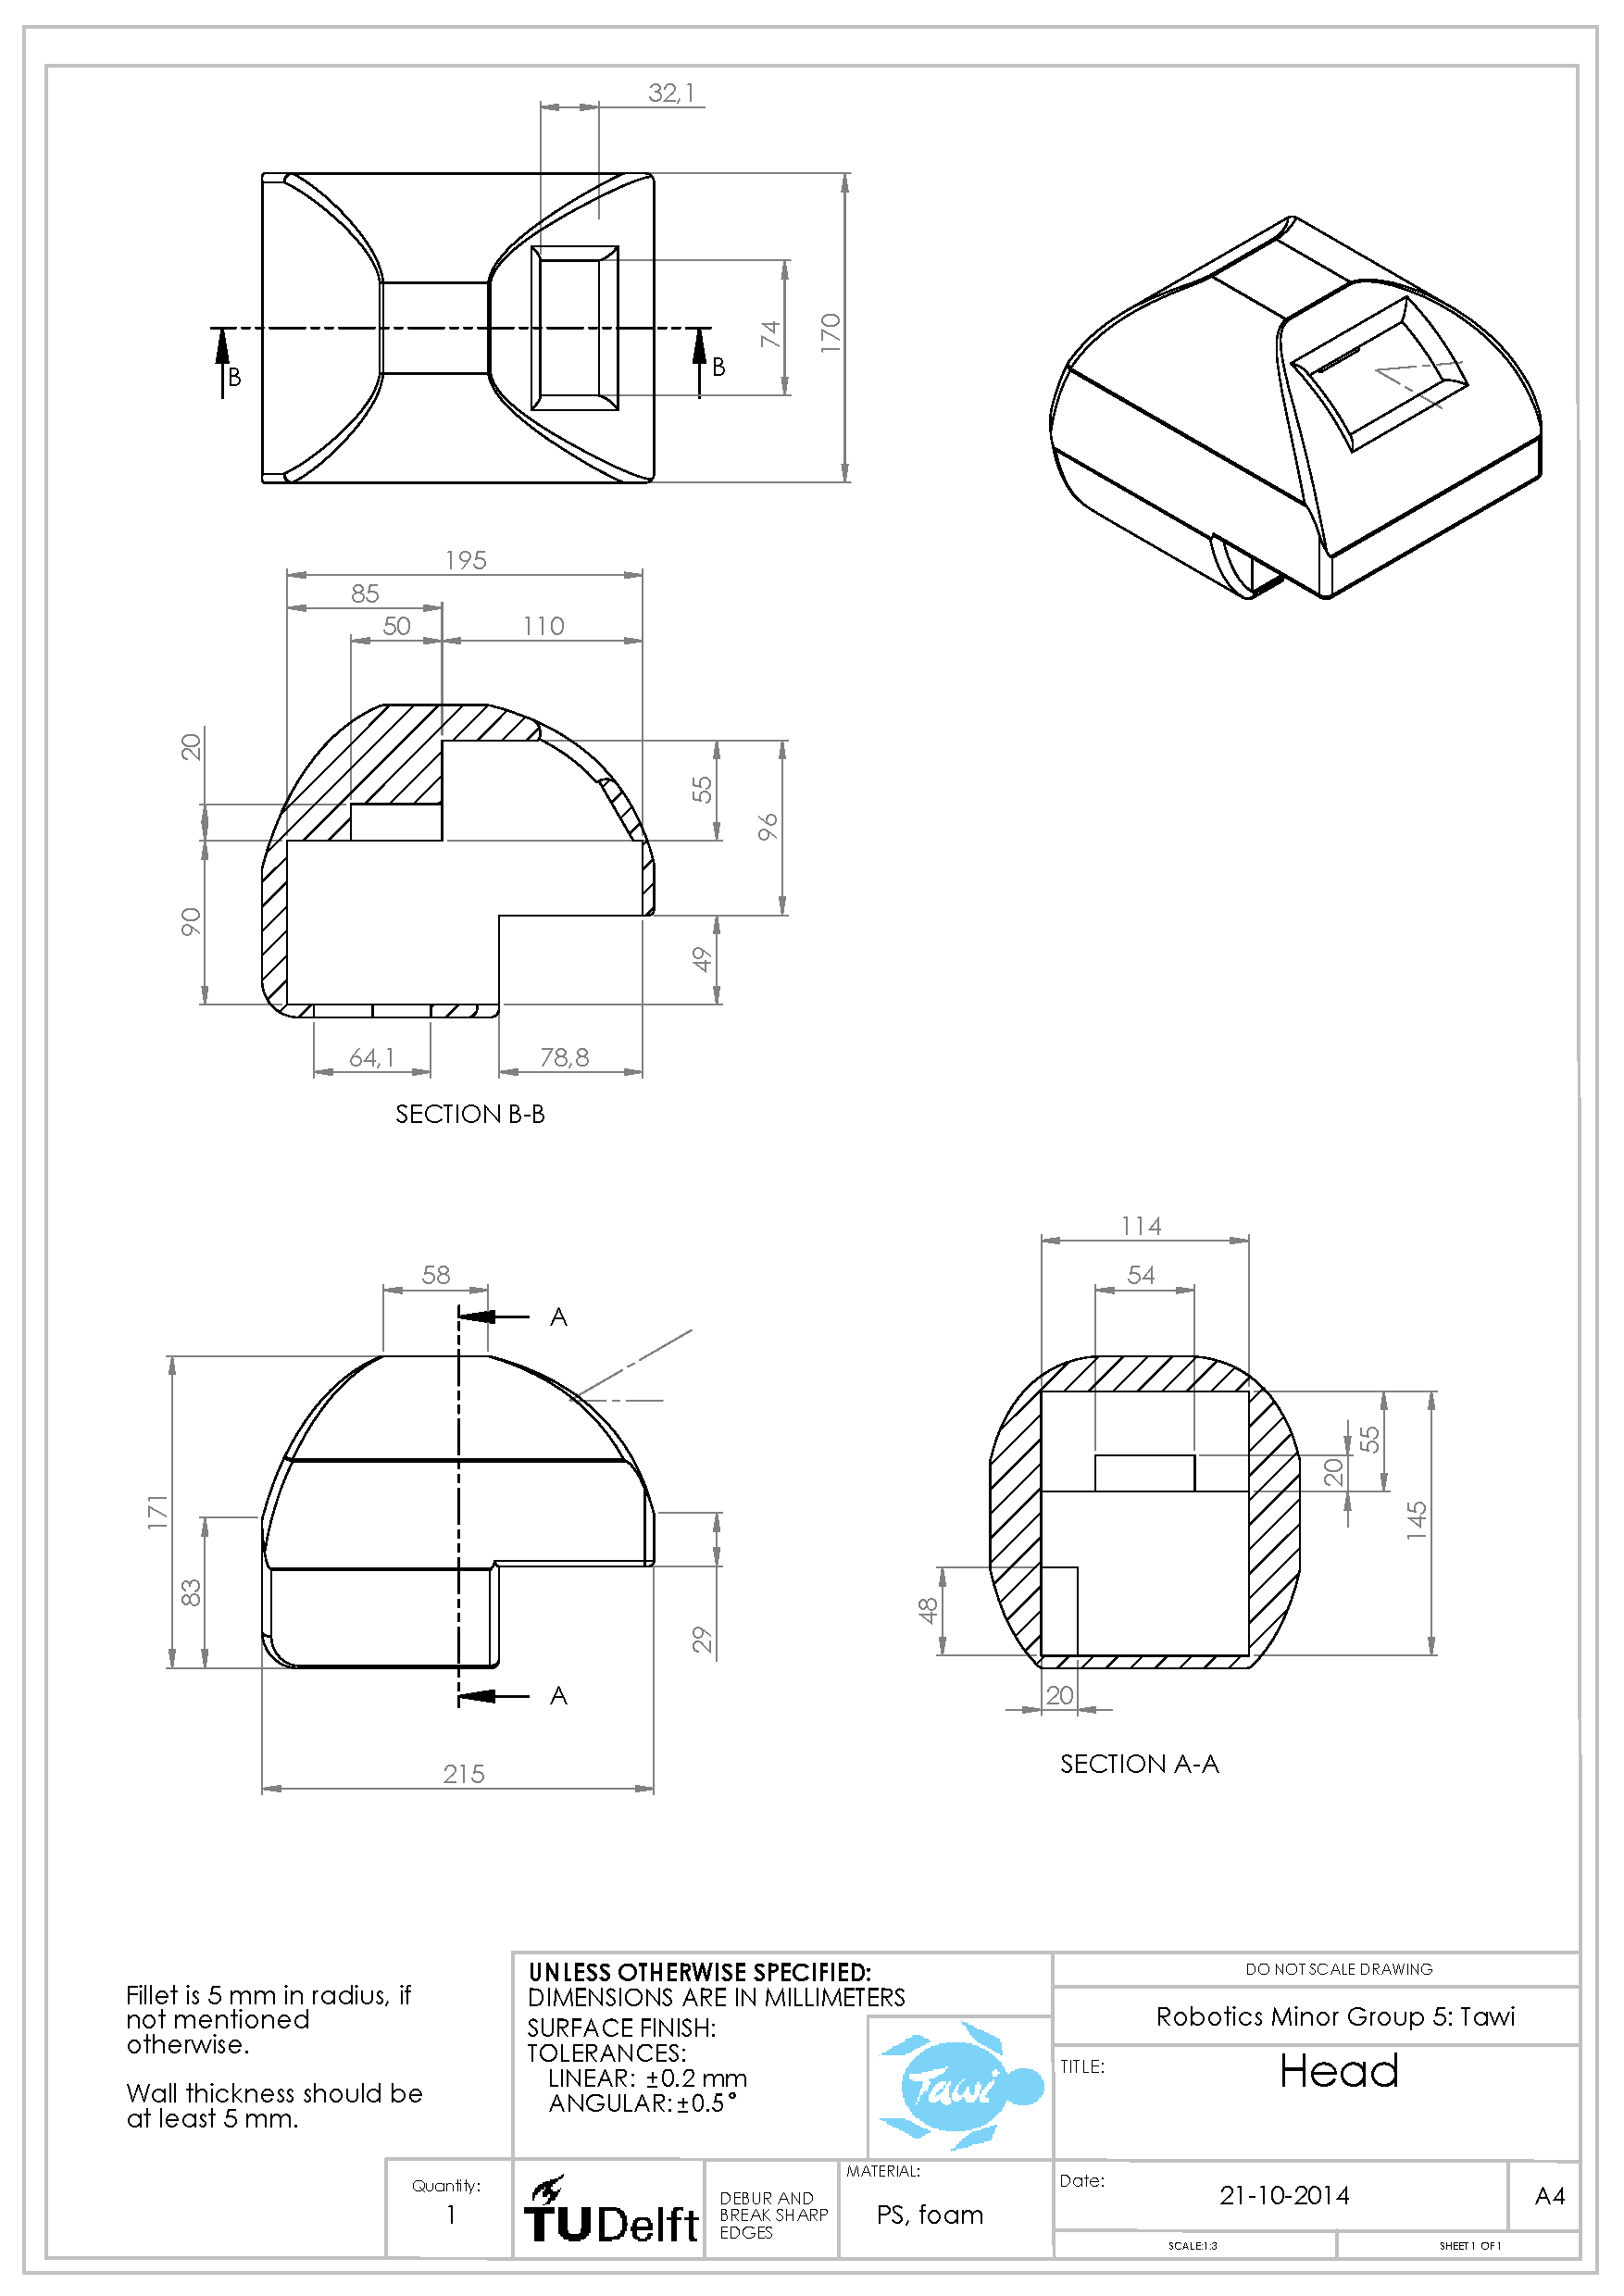
\includepdf[pages={1}]{pdfdrawings/Head.PDF}
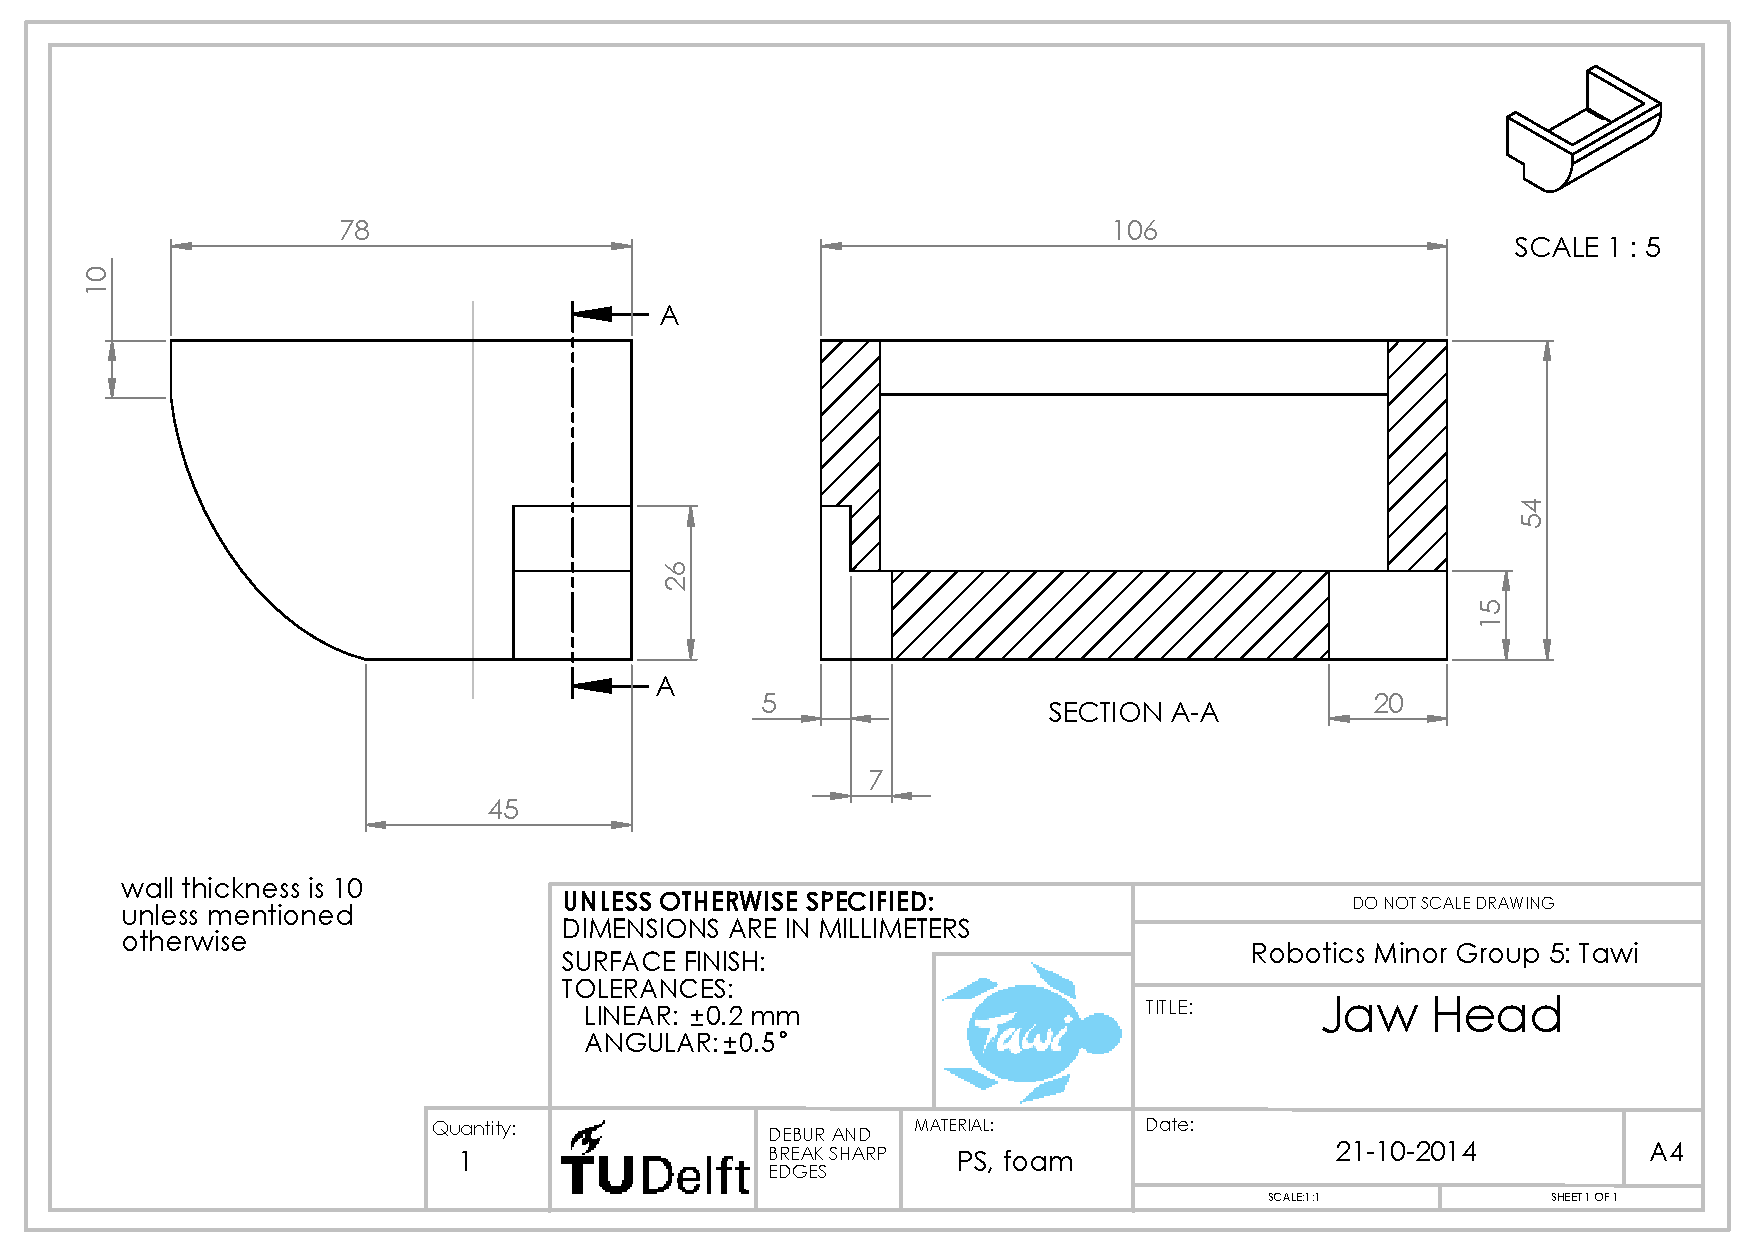
\includepdf[pages={1},landscape=true]{pdfdrawings/Jaw_Head.PDF}
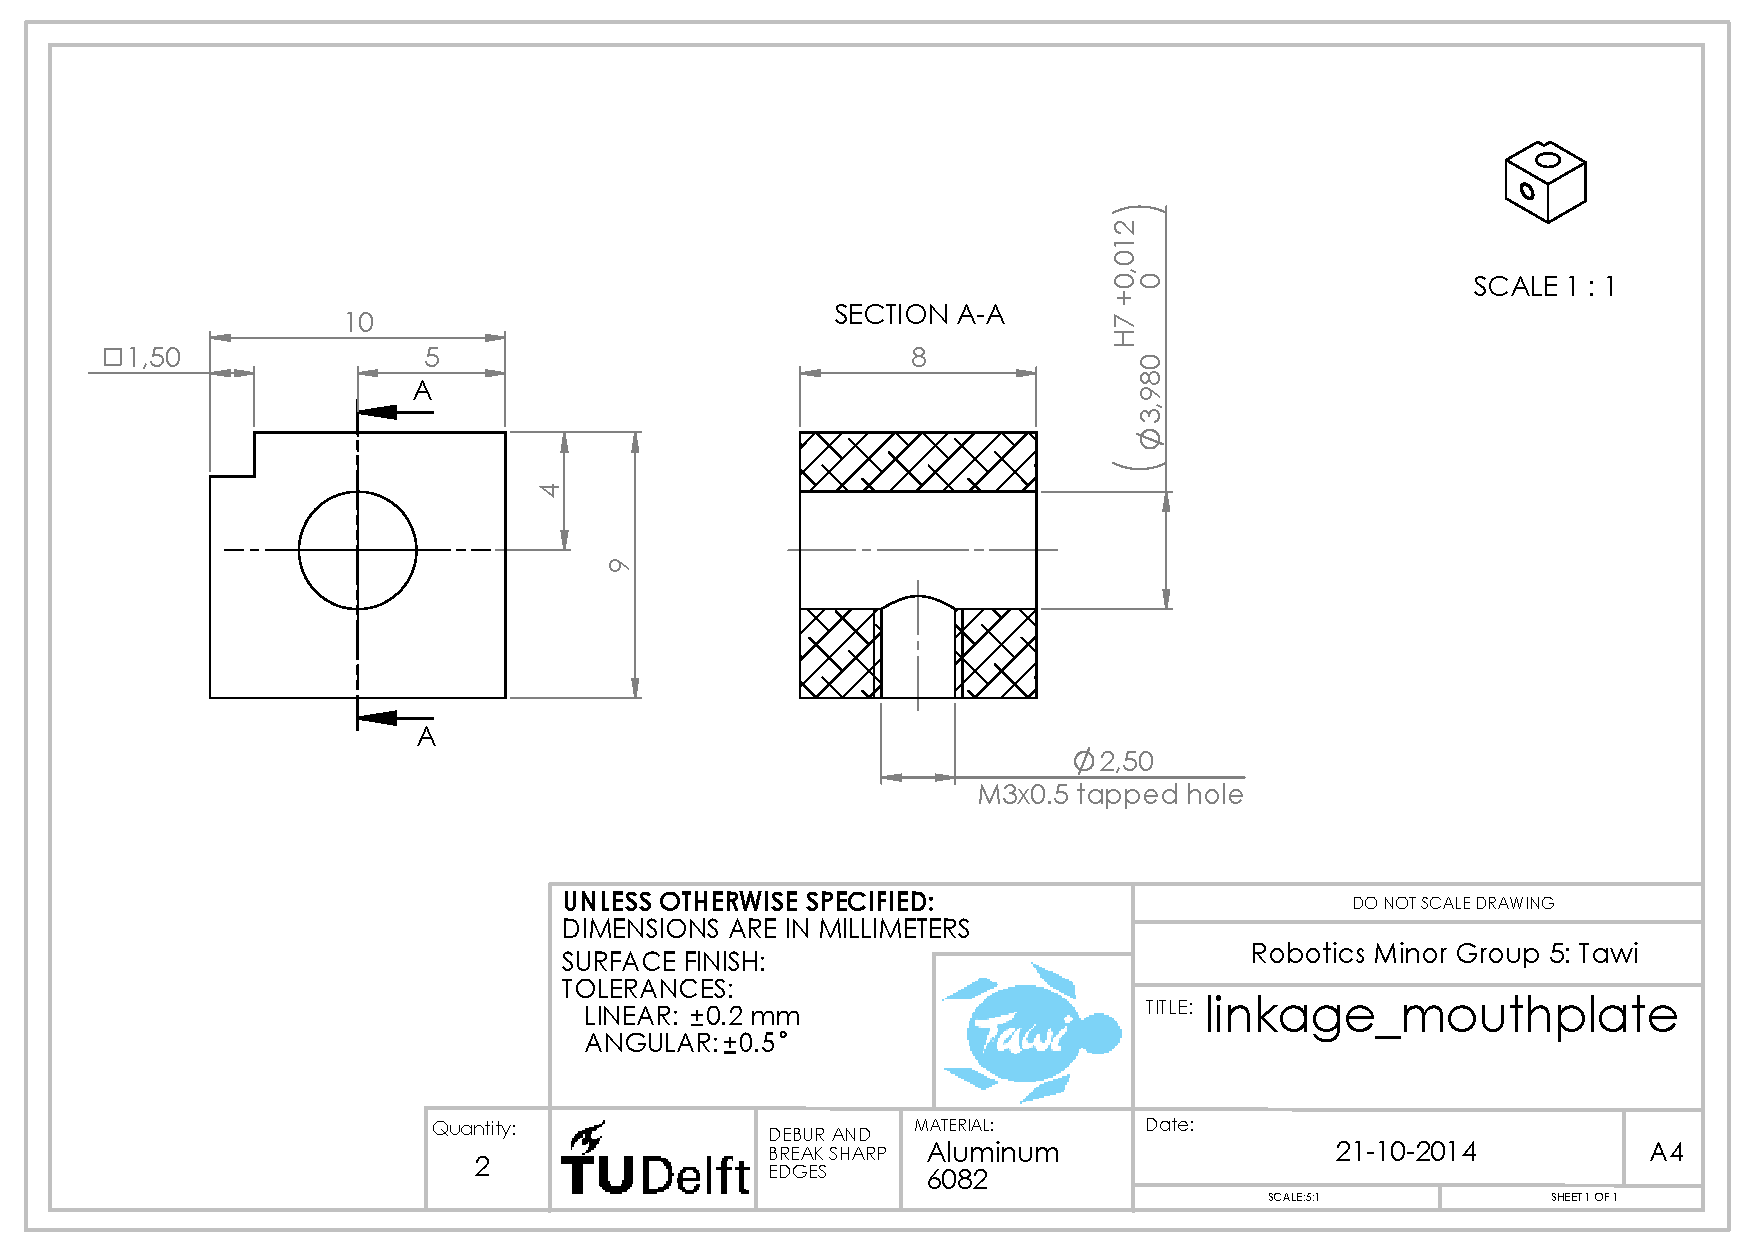
\includepdf[pages={1},landscape=true]{pdfdrawings/linkage_mouthplate.PDF}
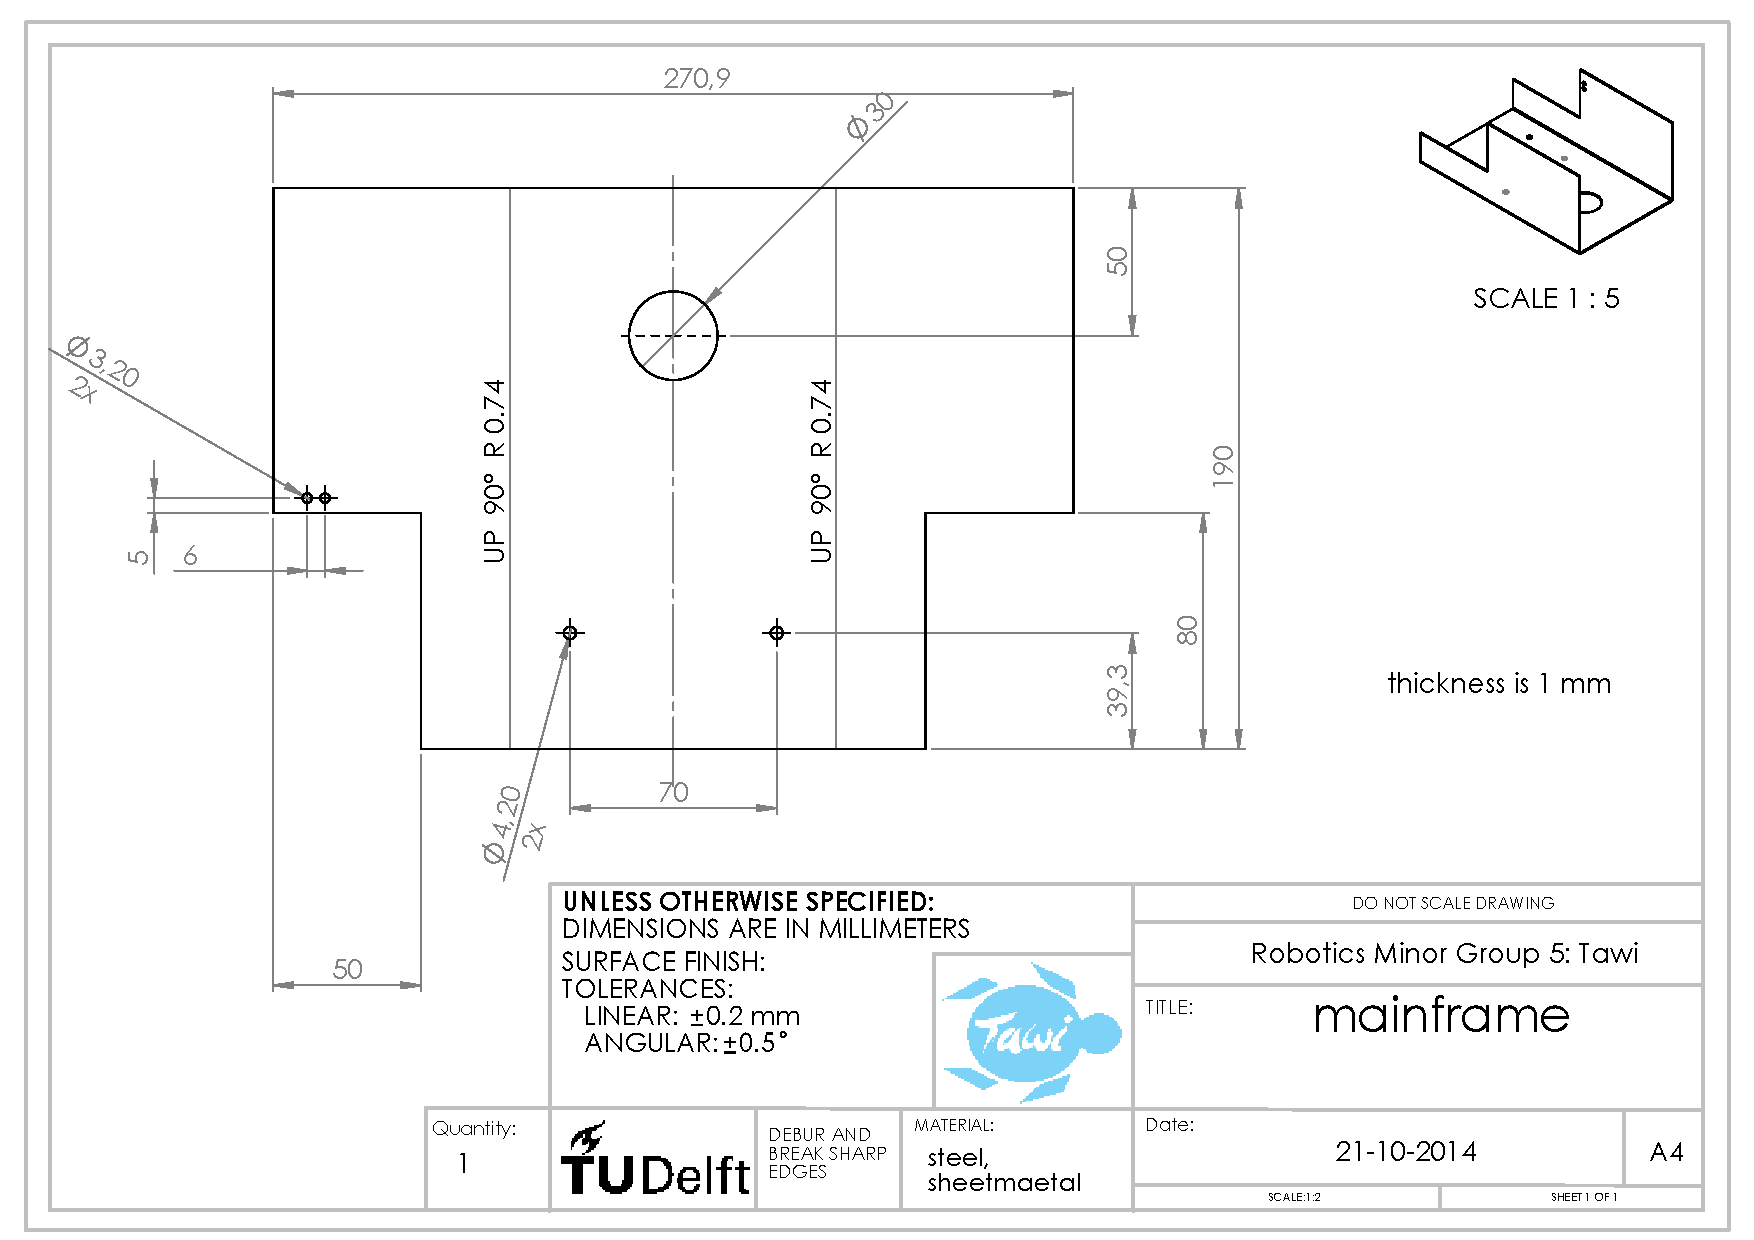
\includepdf[pages={1},landscape=true]{pdfdrawings/mainframe.PDF}
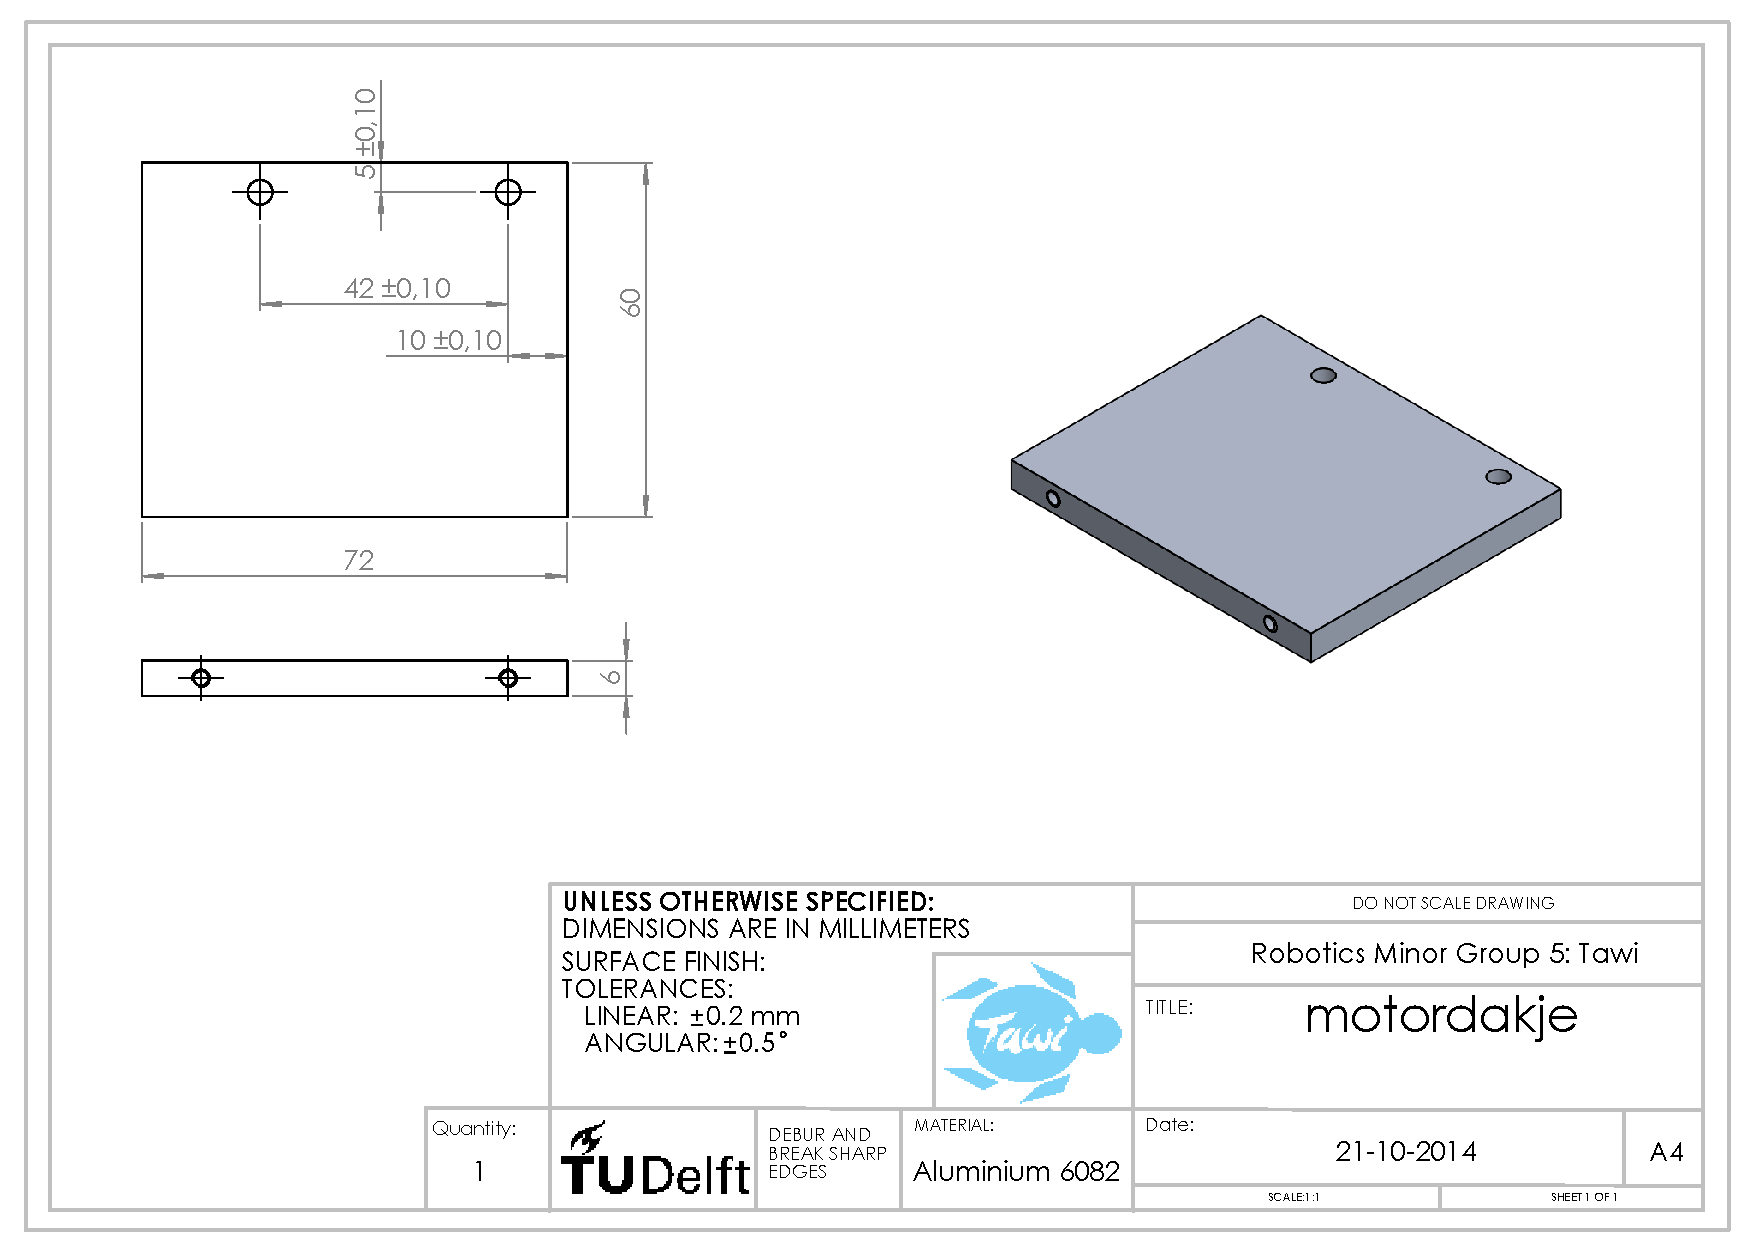
\includepdf[pages={1},landscape=true]{pdfdrawings/motordakje.PDF}
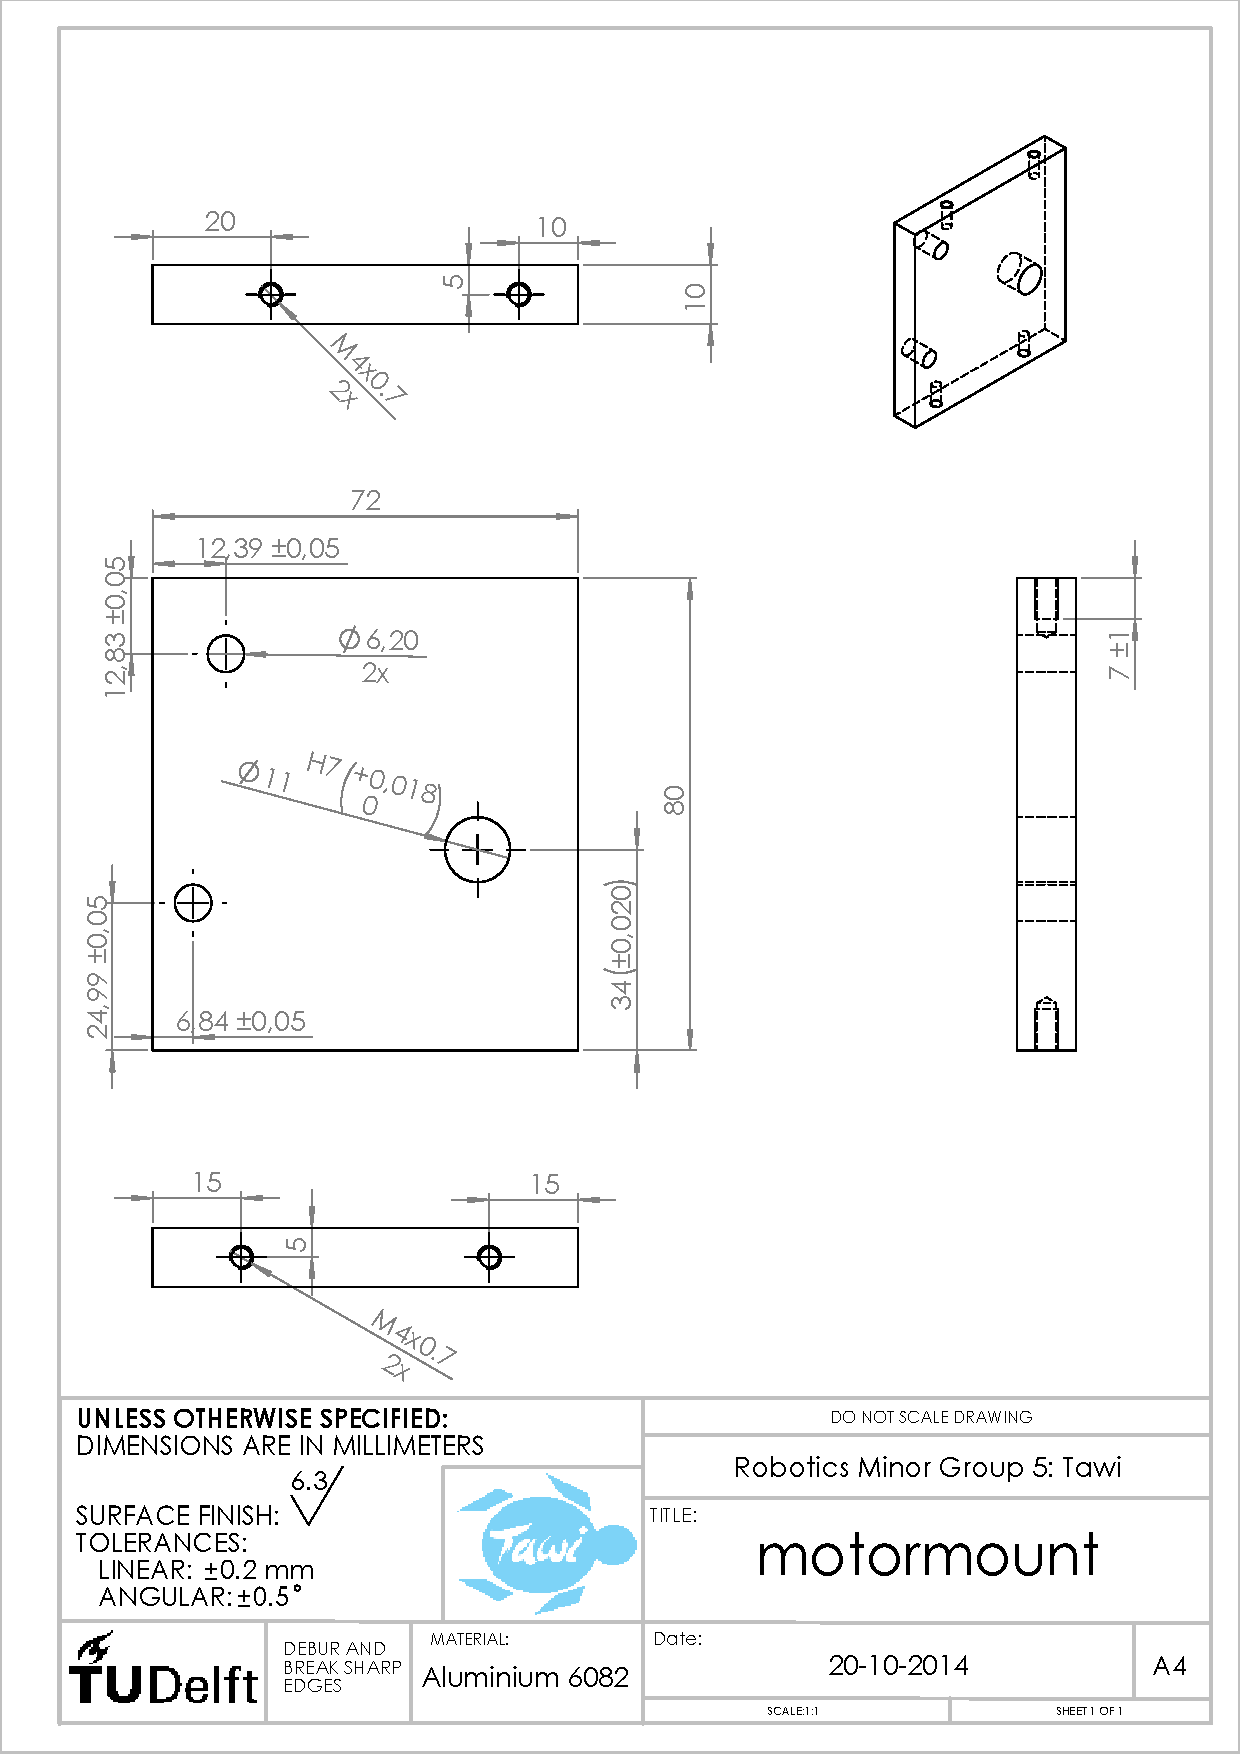
\includepdf[pages={1}]{pdfdrawings/motormount.PDF}
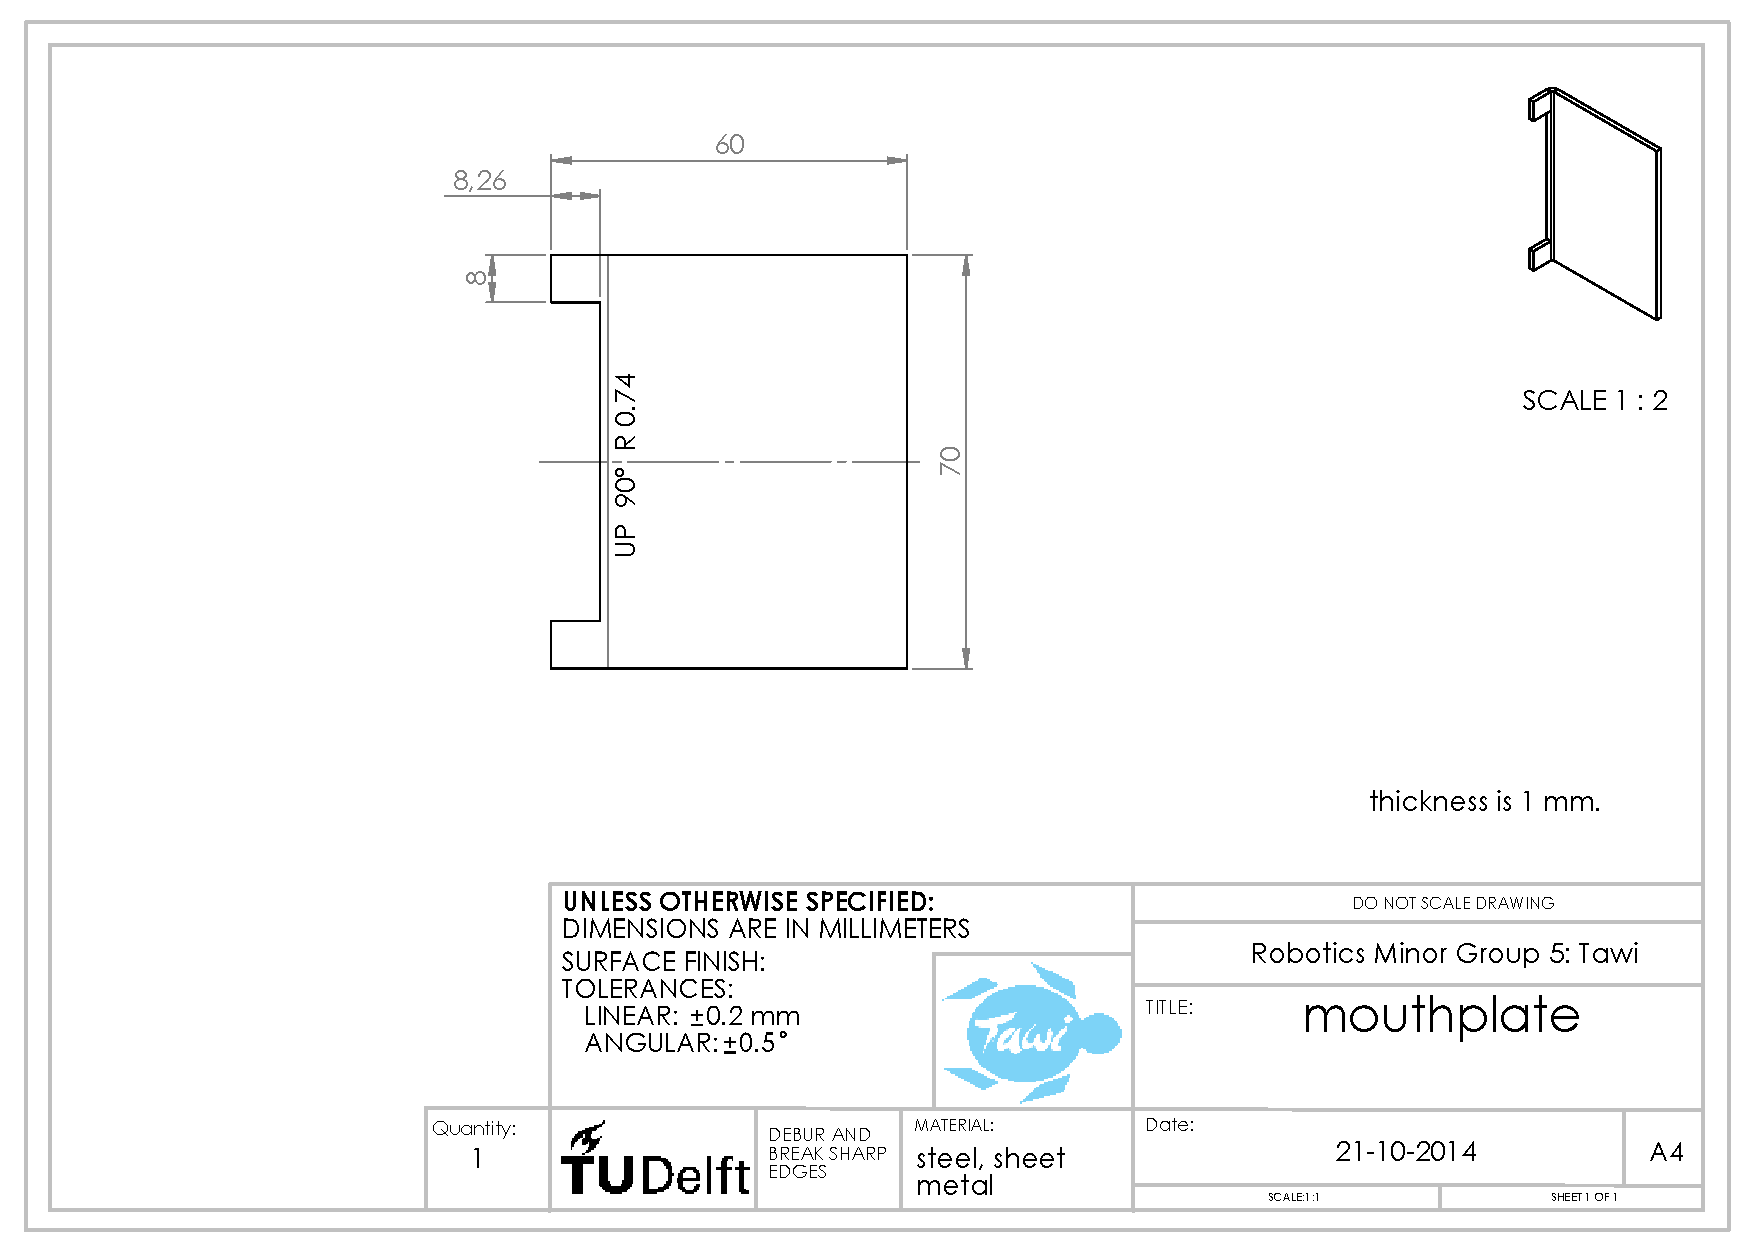
\includepdf[pages={1},landscape=true]{pdfdrawings/mouthplate.PDF}
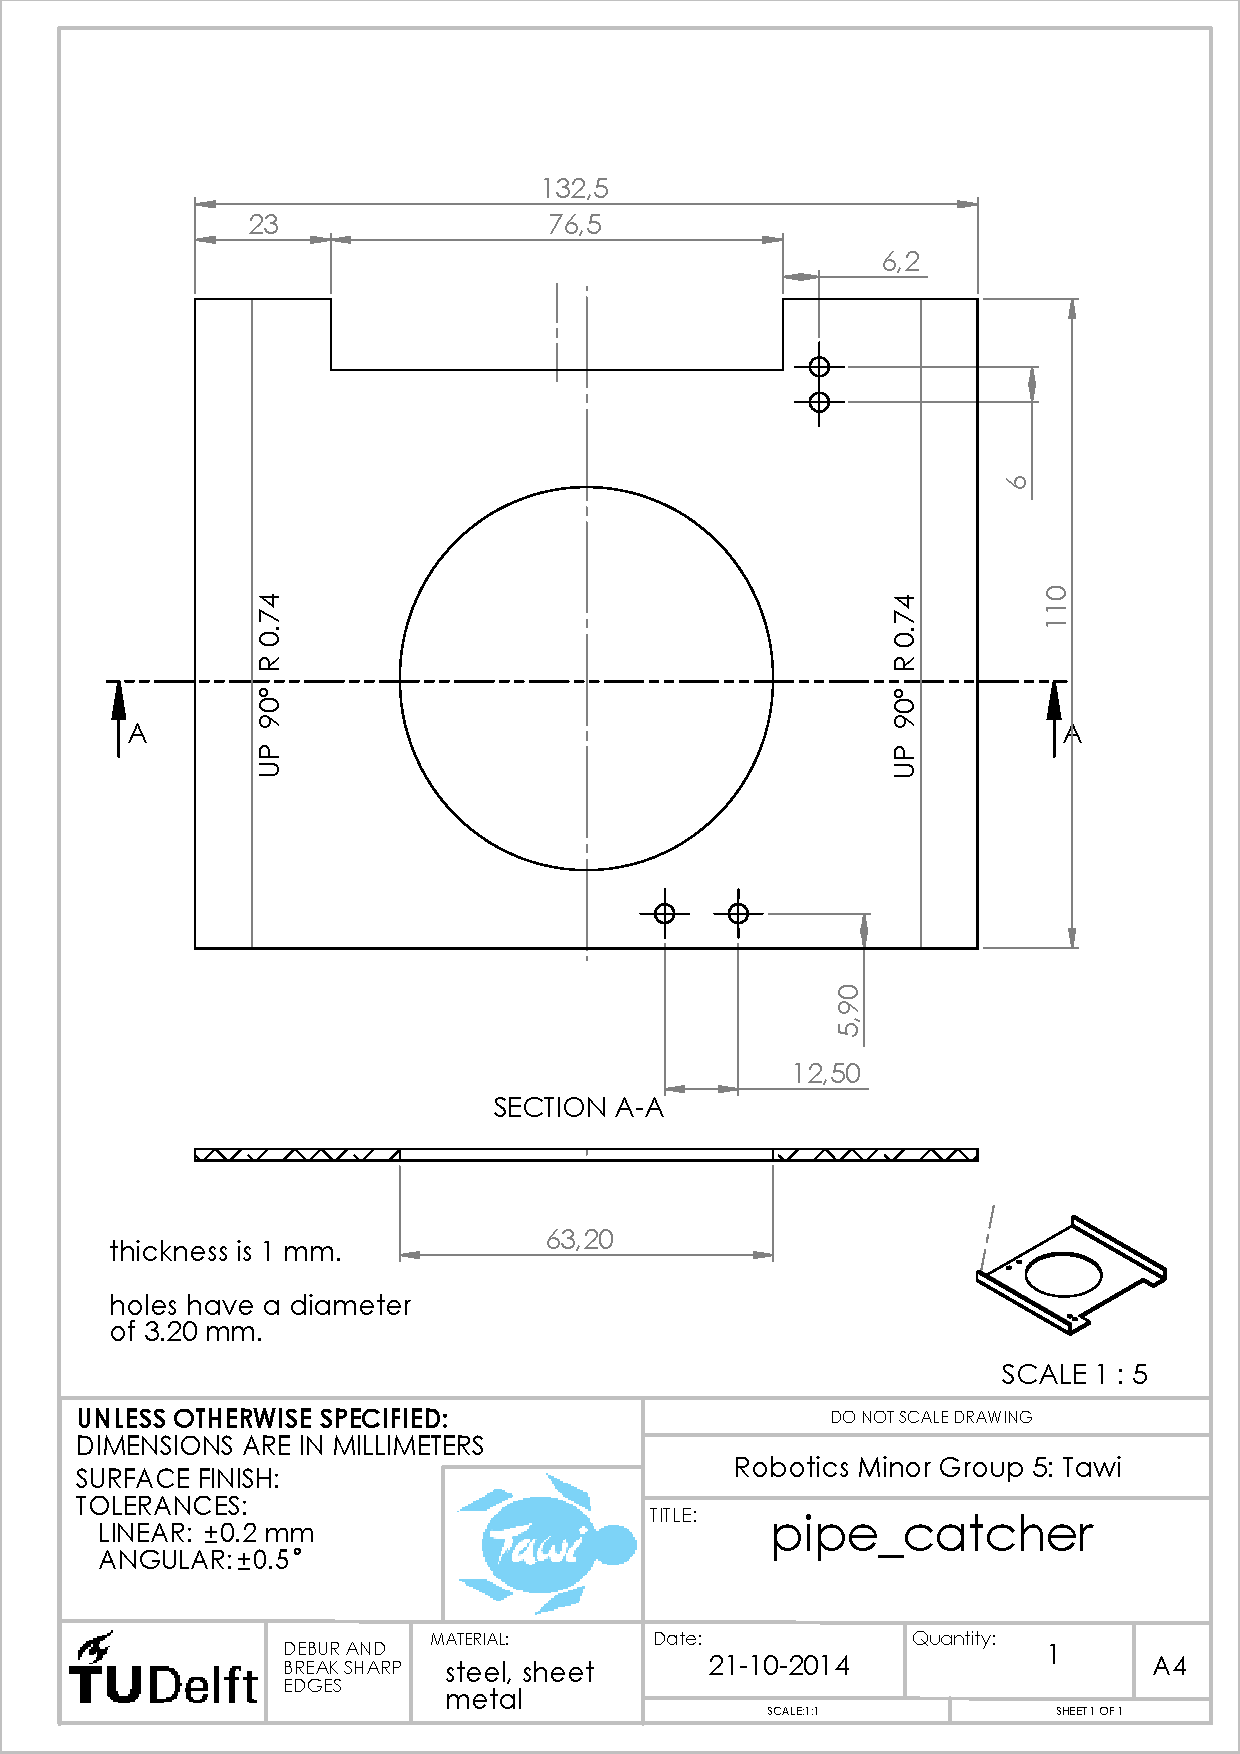
\includepdf[pages={1}]{pdfdrawings/pipe_catcher.PDF}
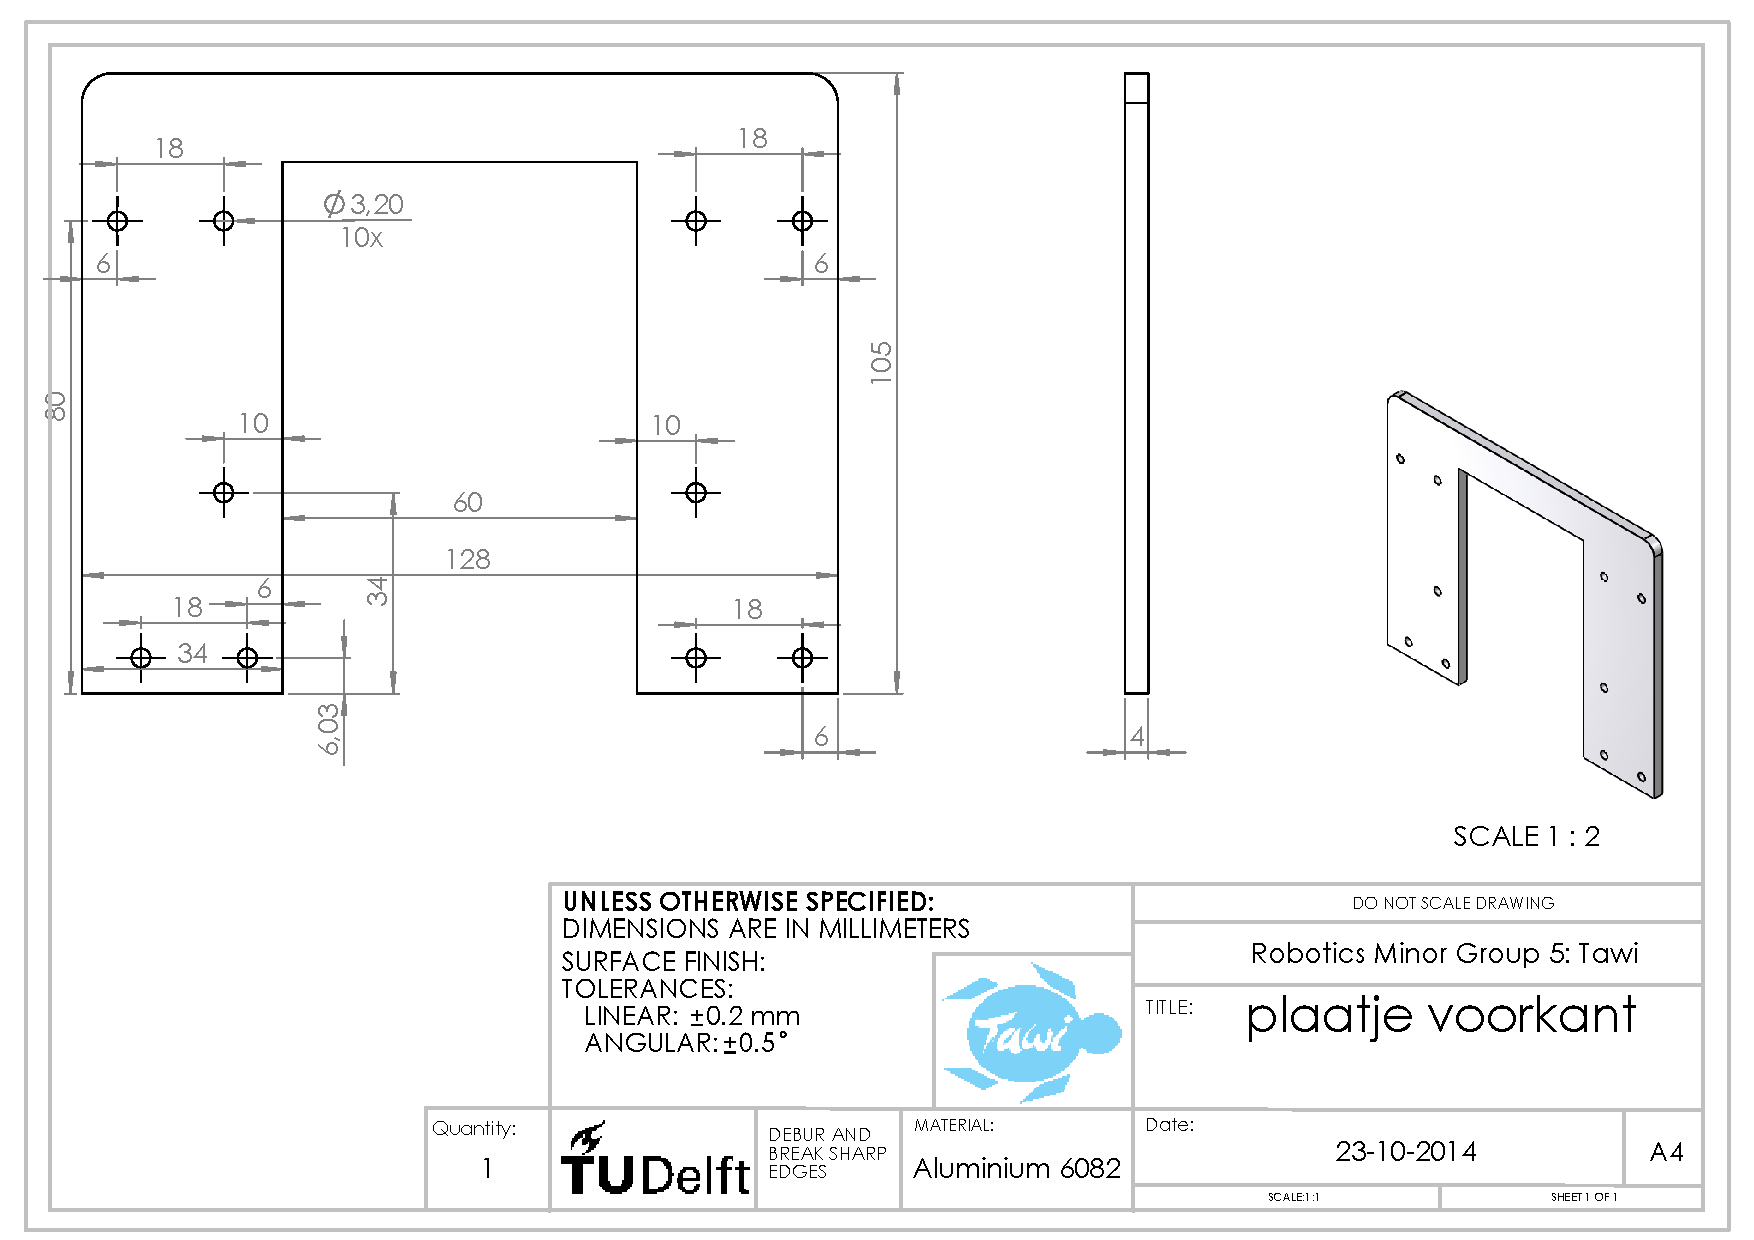
\includepdf[pages={1},landscape=true]{pdfdrawings/plaatje_voorkant.PDF}
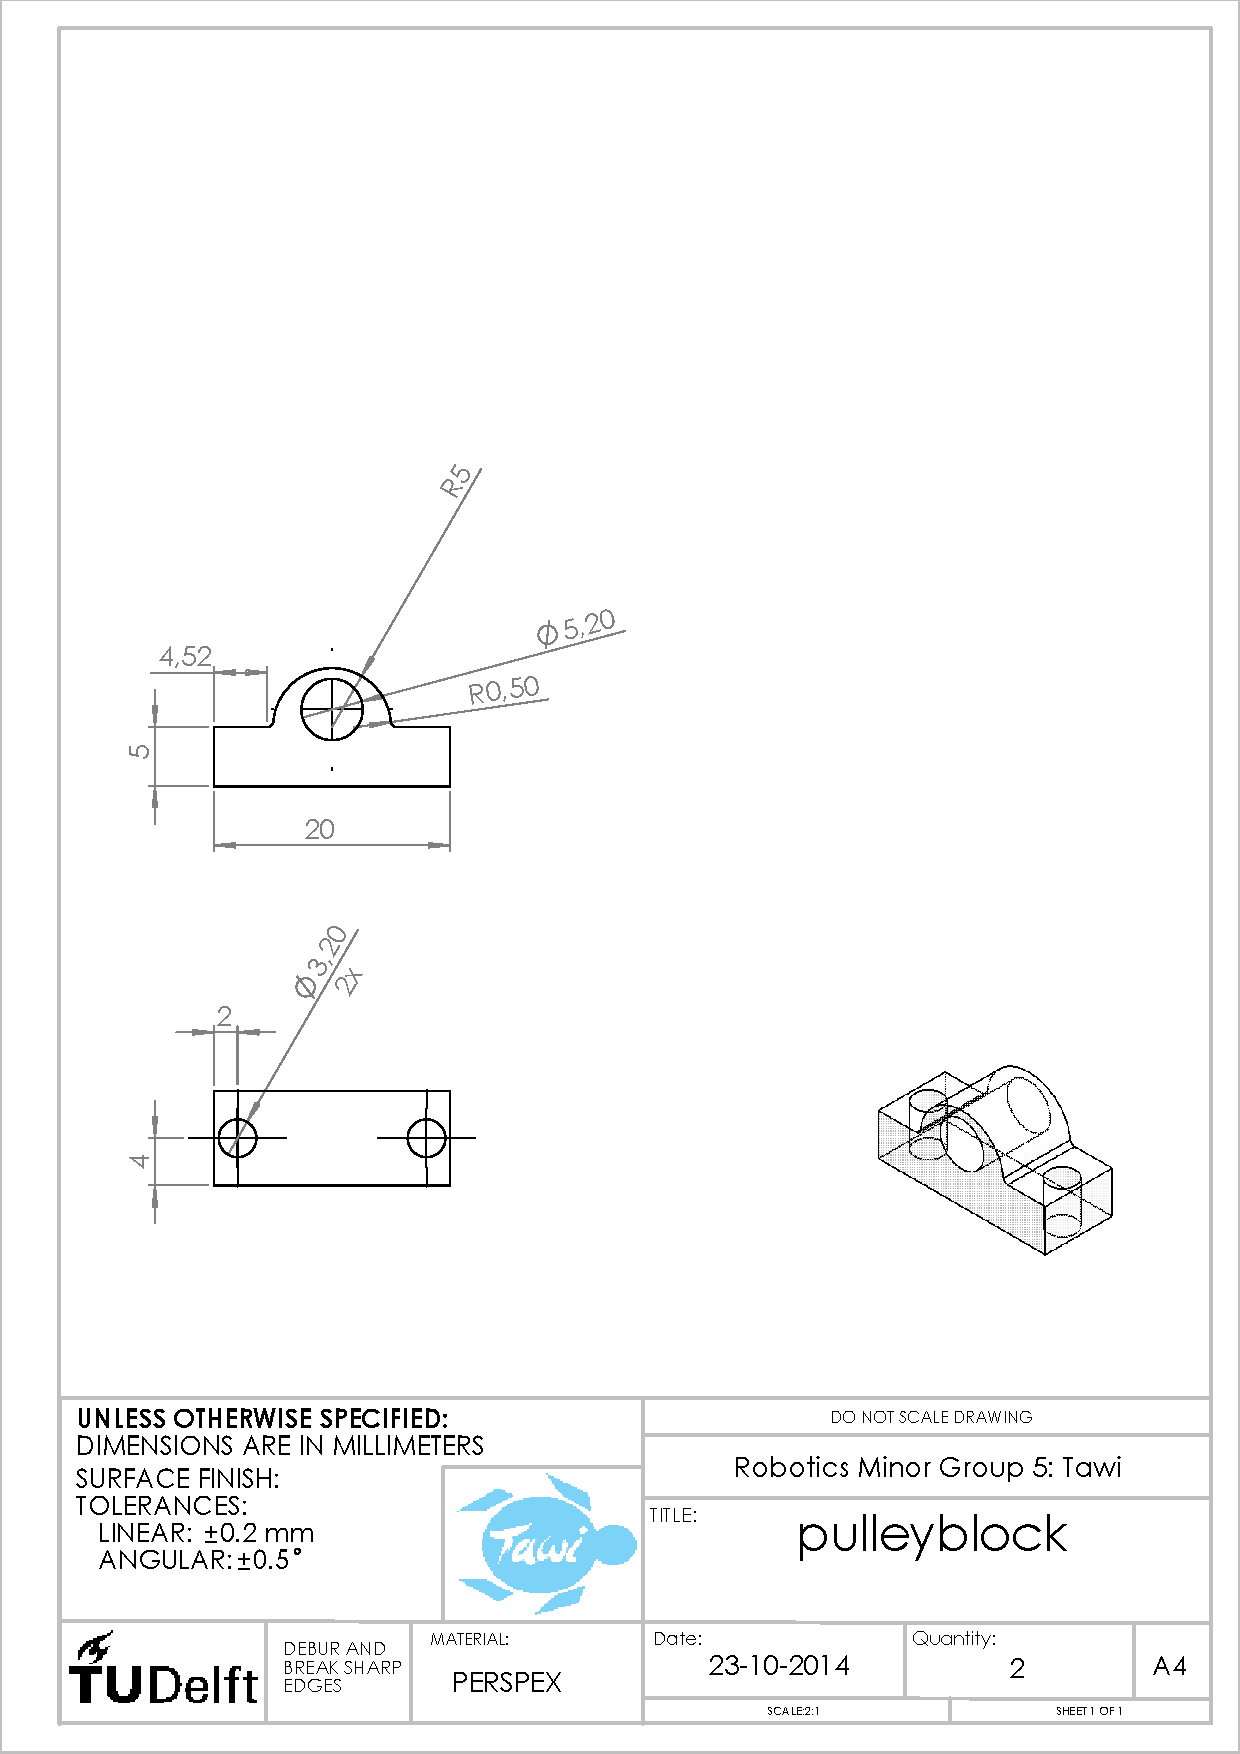
\includepdf[pages={1}]{pdfdrawings/pulleyblock.PDF}
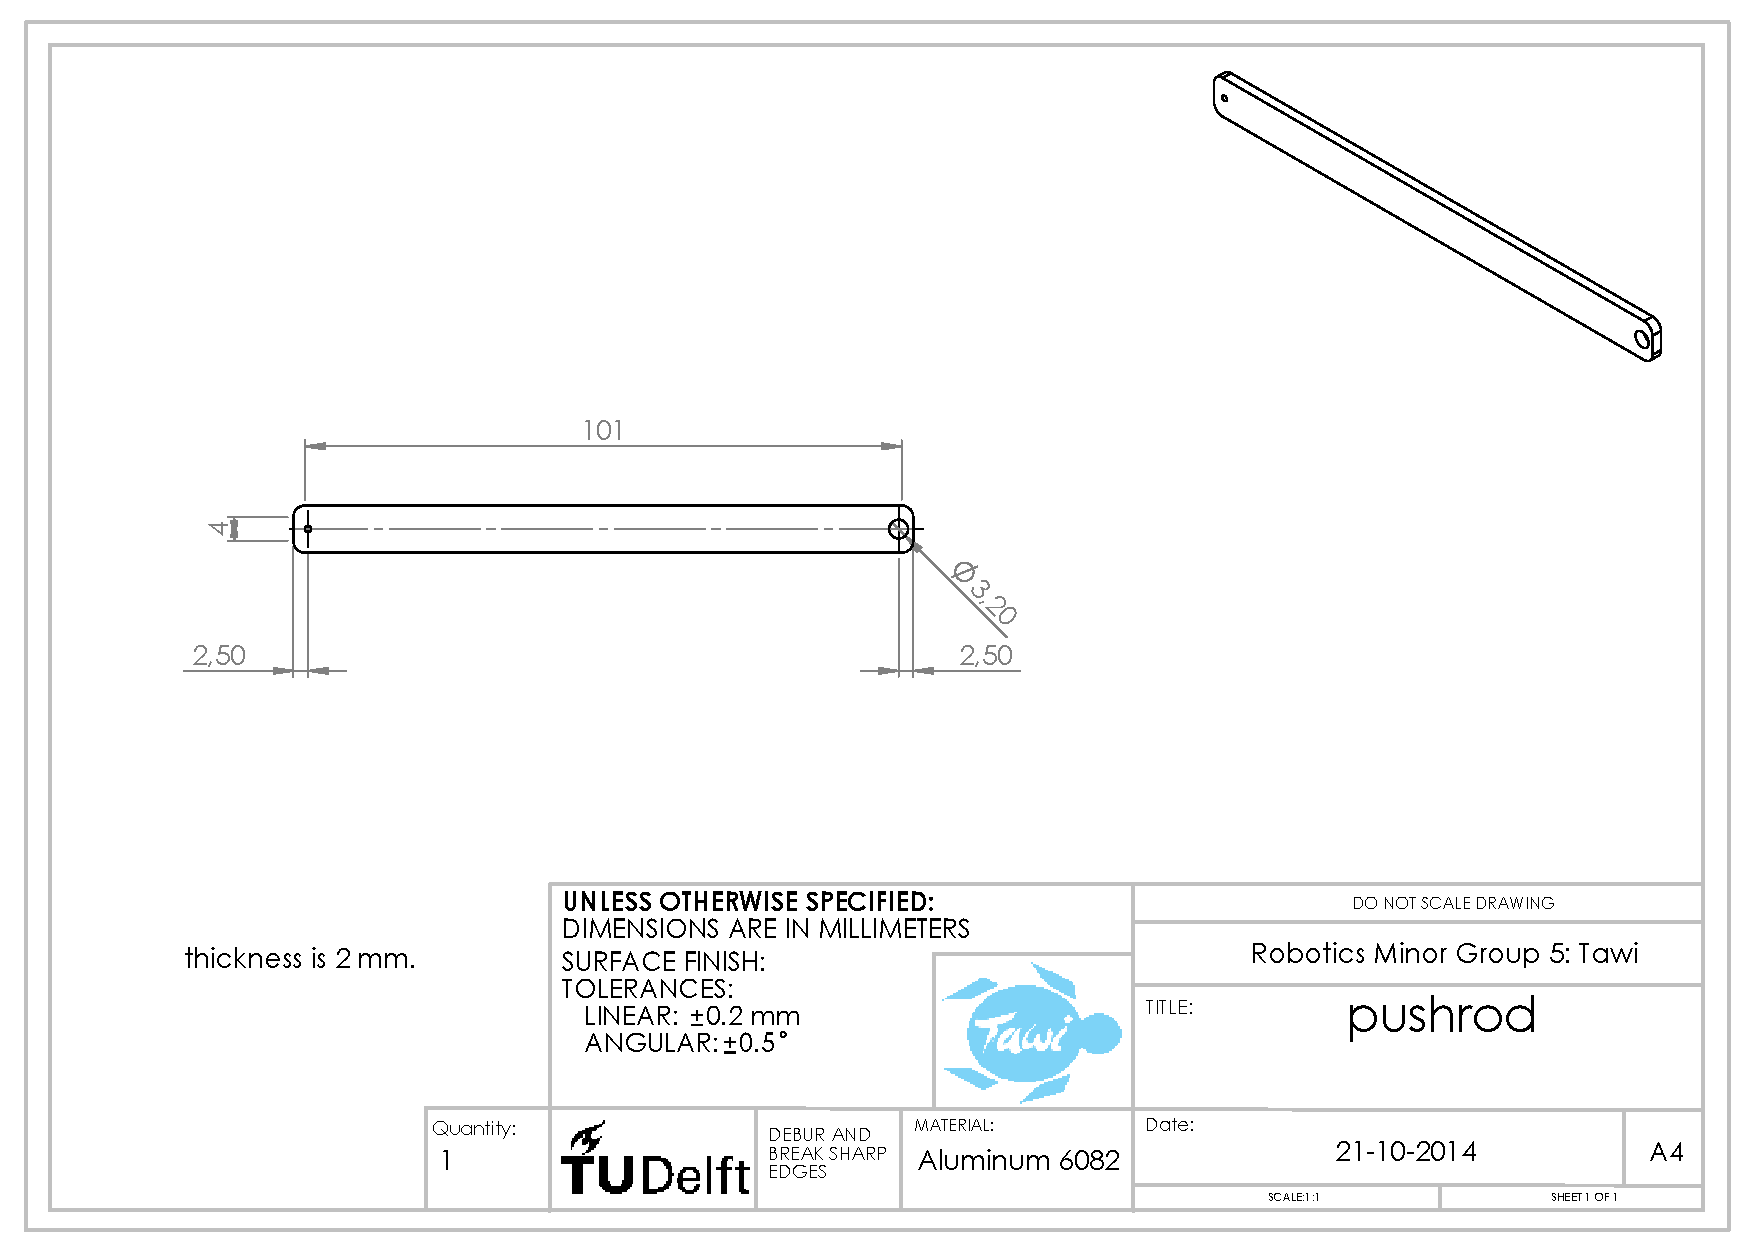
\includepdf[pages={1},landscape=true]{pdfdrawings/pushrod.PDF}
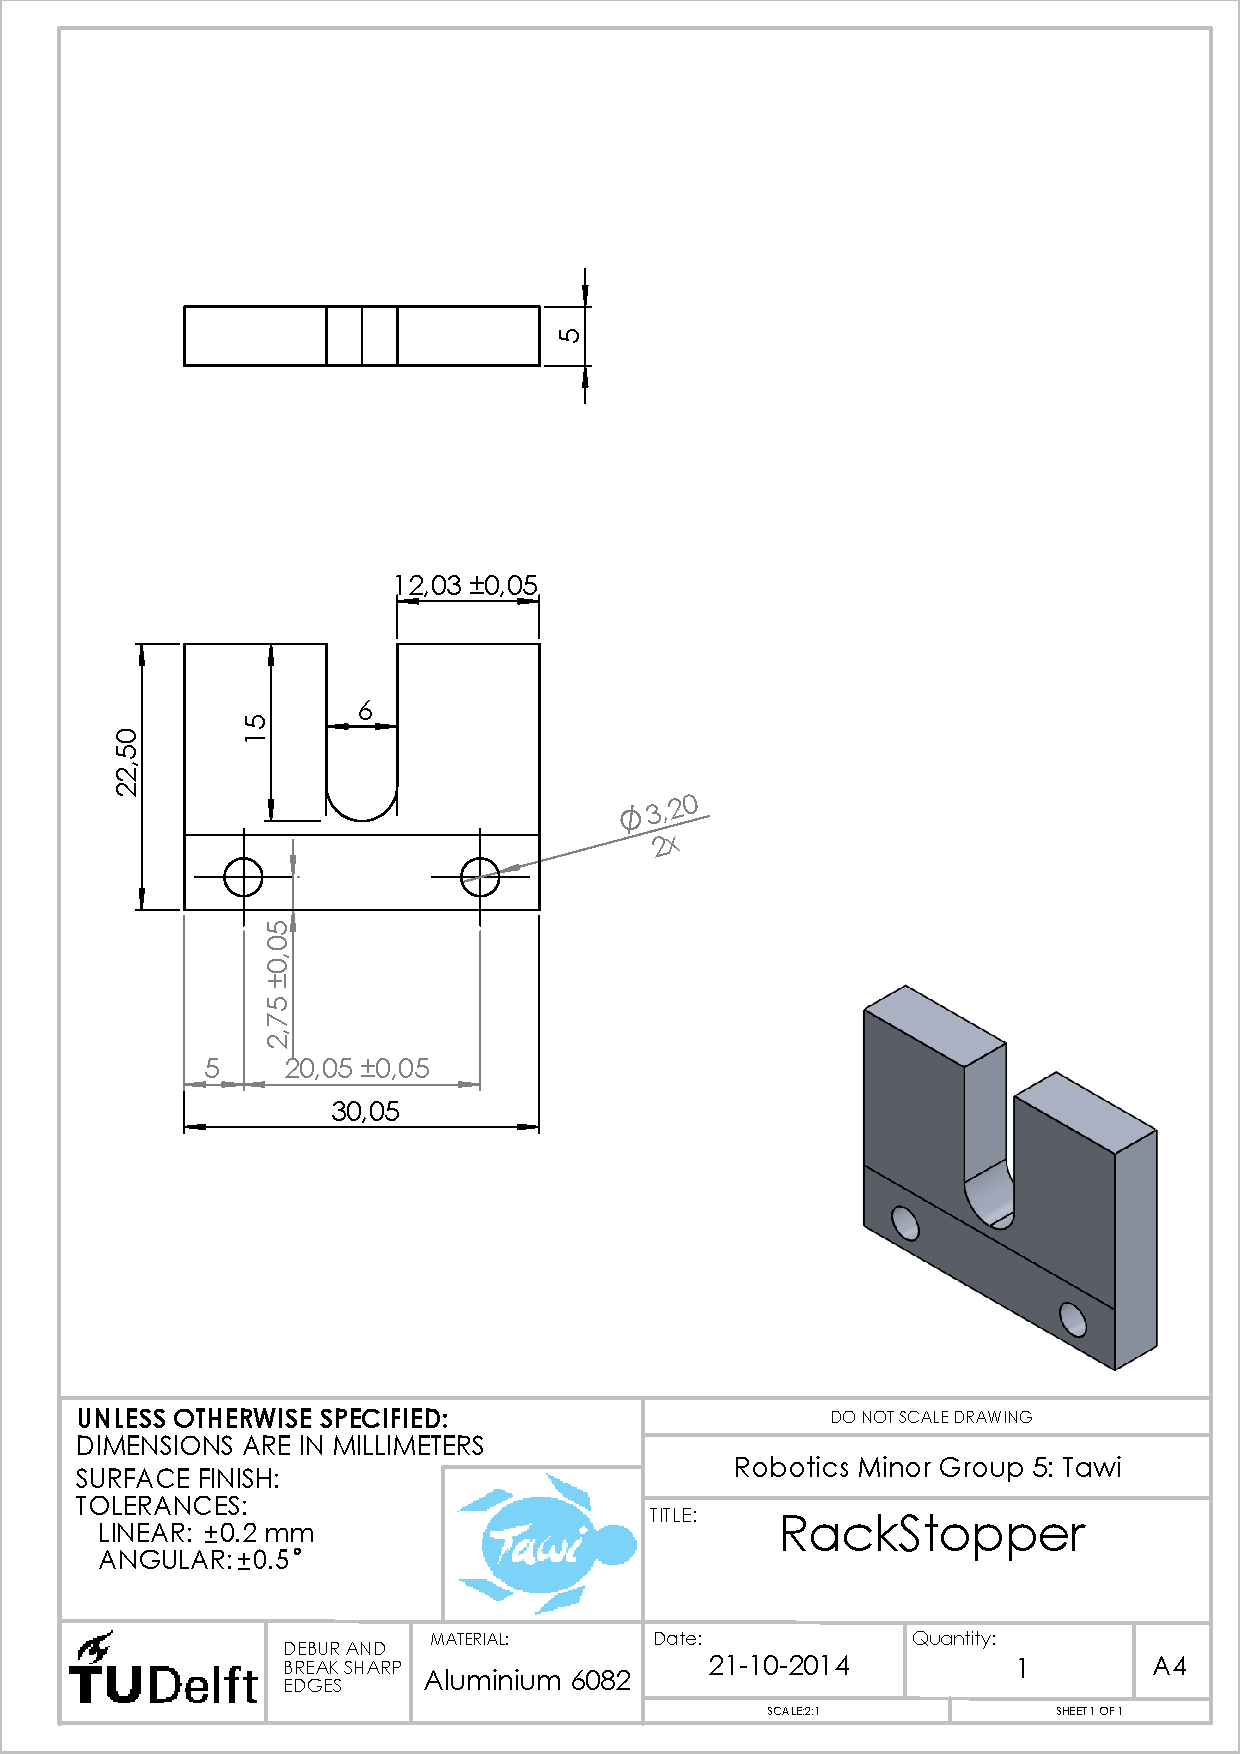
\includepdf[pages={1}]{pdfdrawings/RackStopper.PDF}
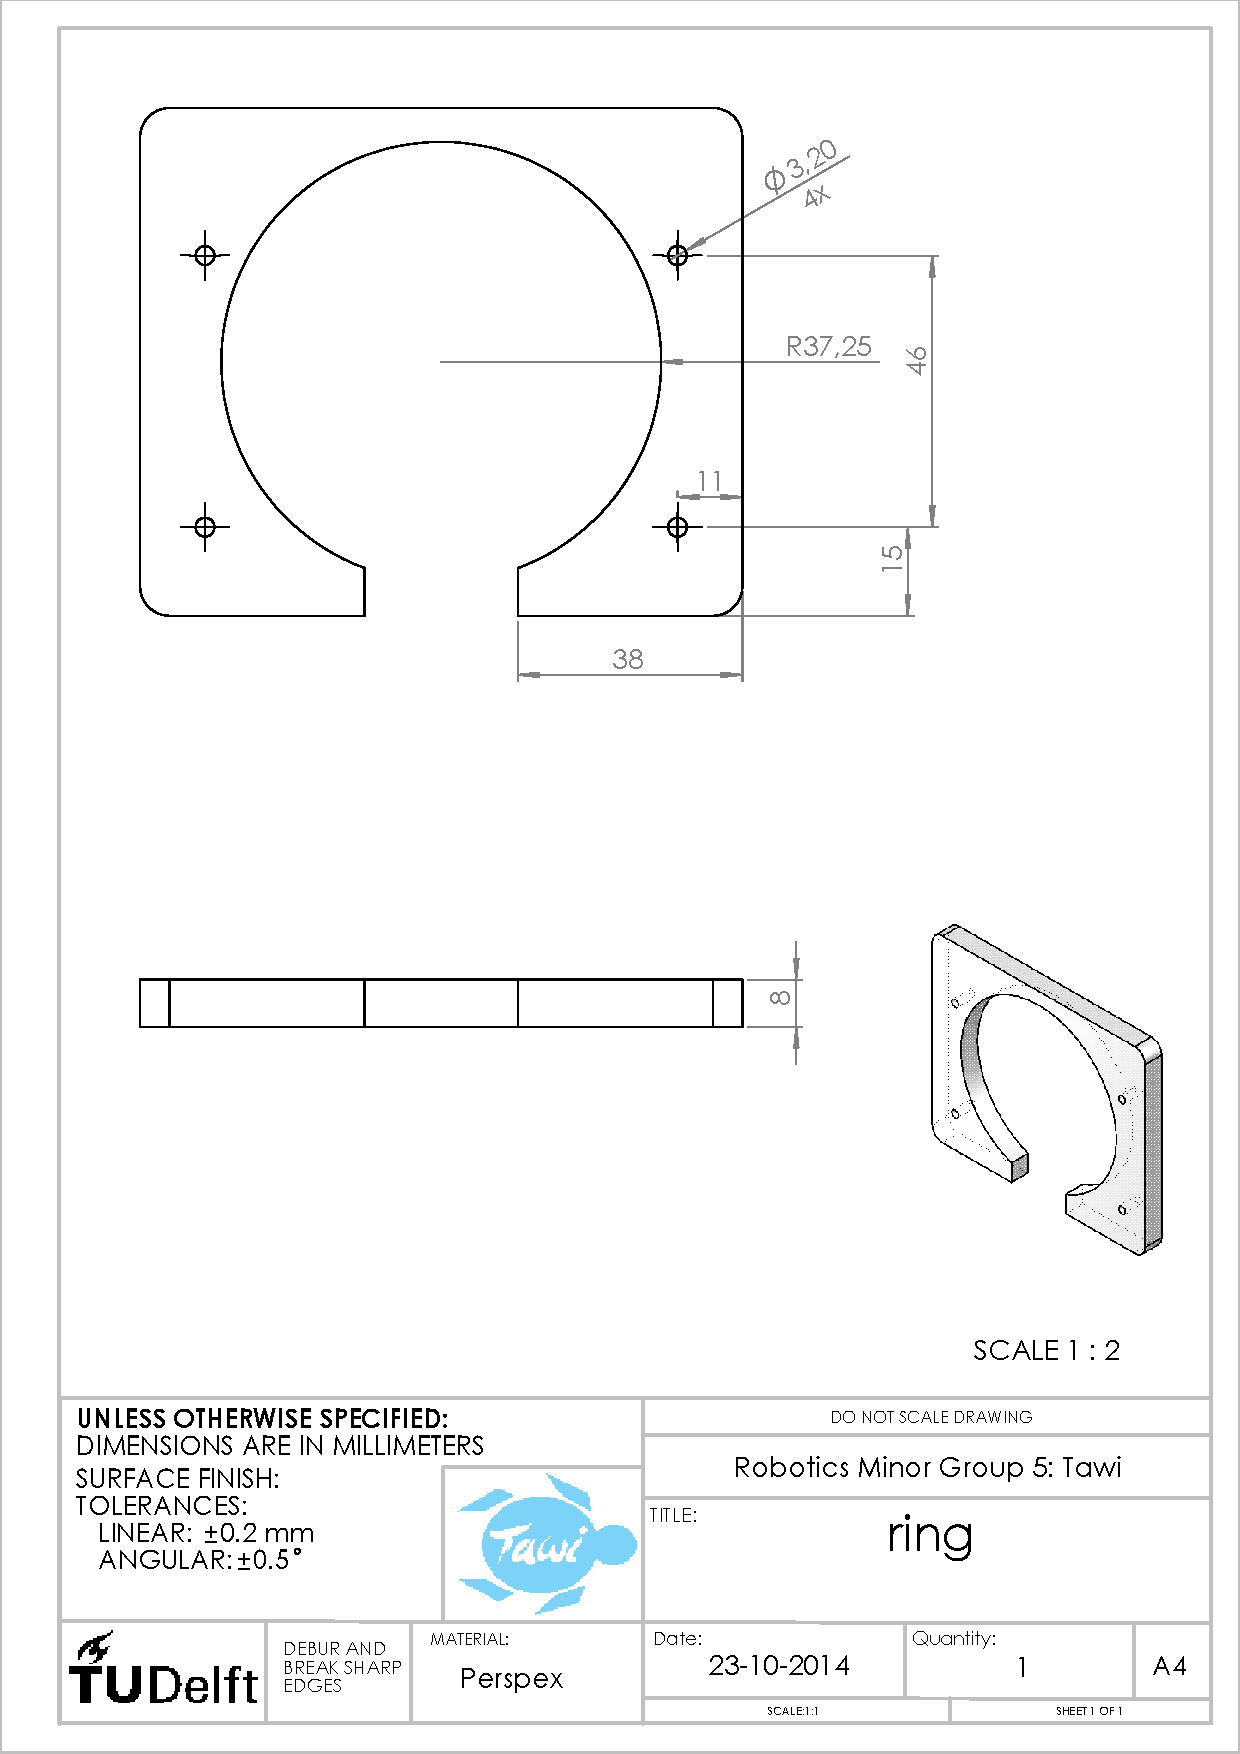
\includepdf[pages={1}]{pdfdrawings/ring.PDF}
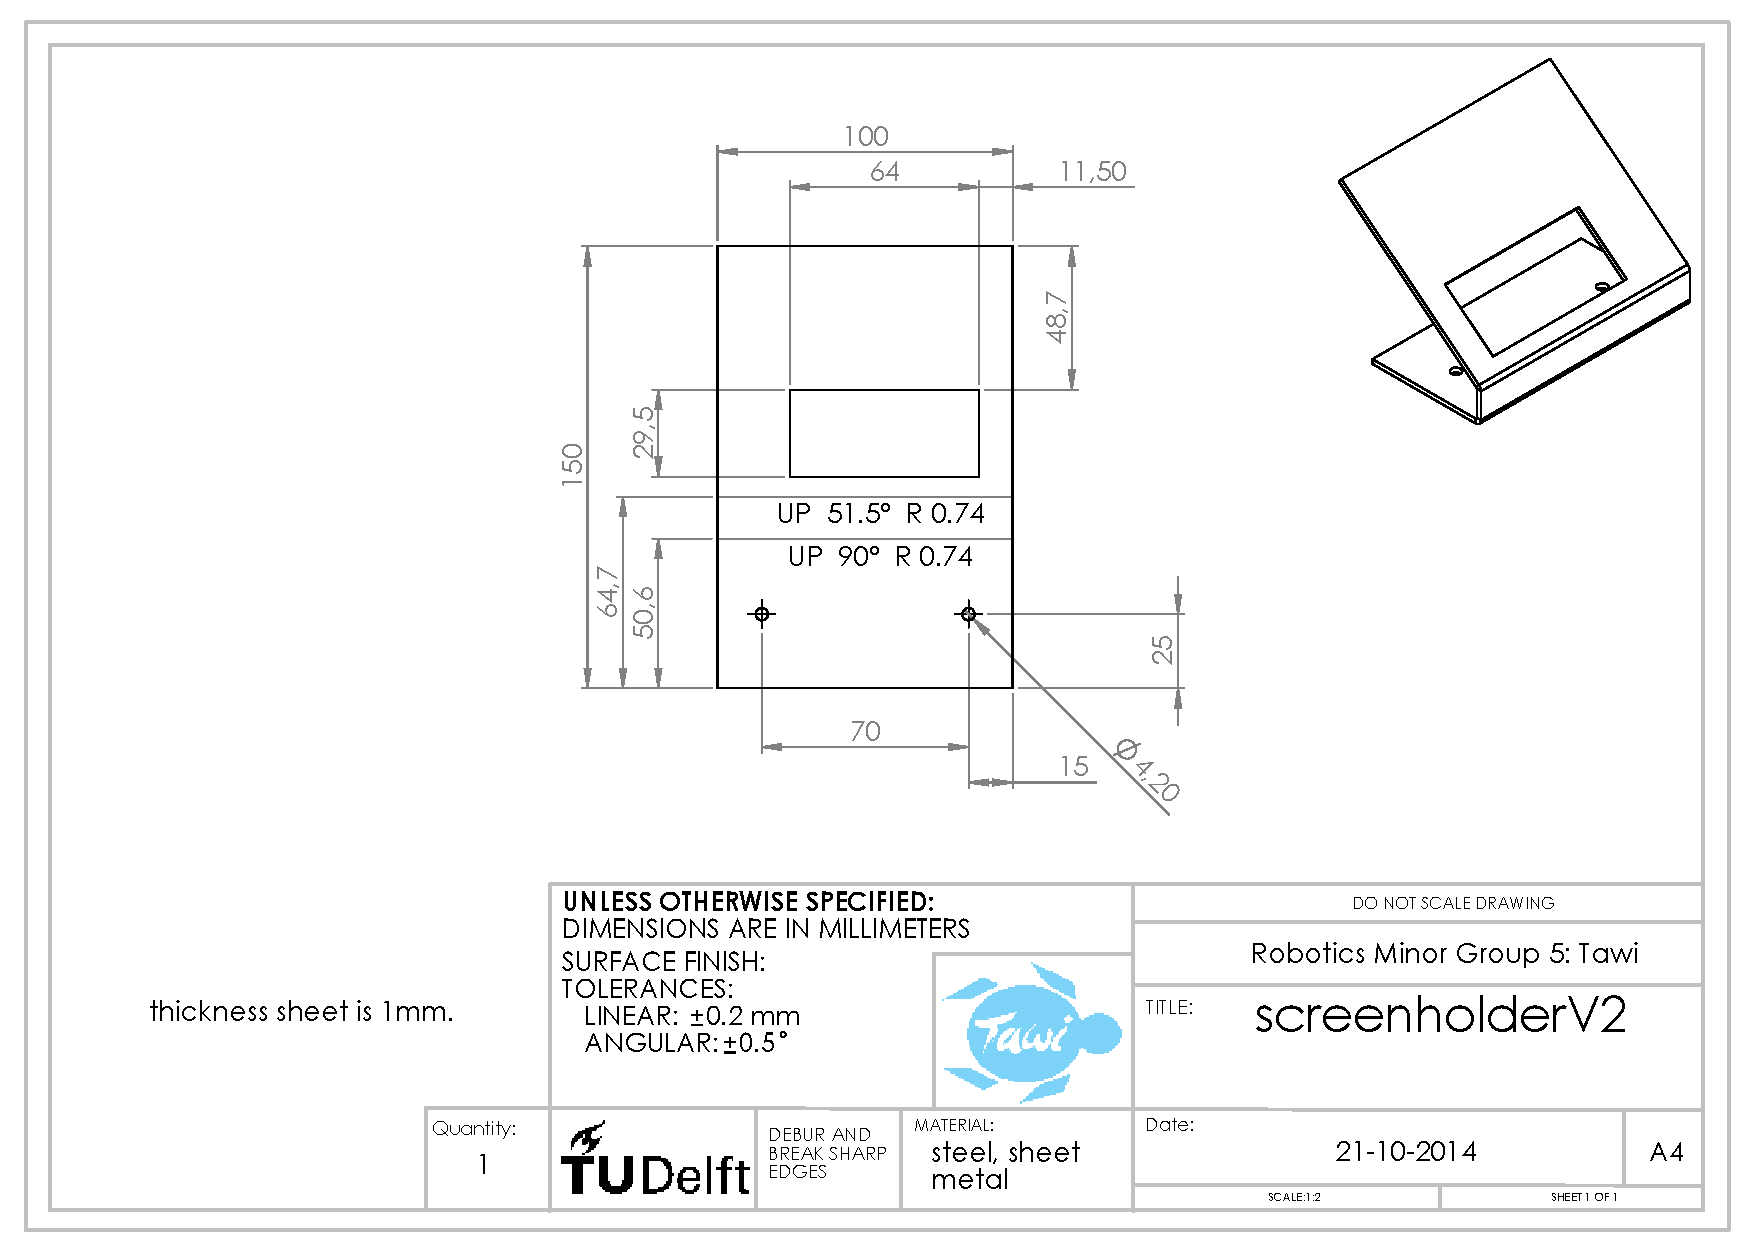
\includepdf[pages={1},landscape=true]{pdfdrawings/screenholderV2.PDF}
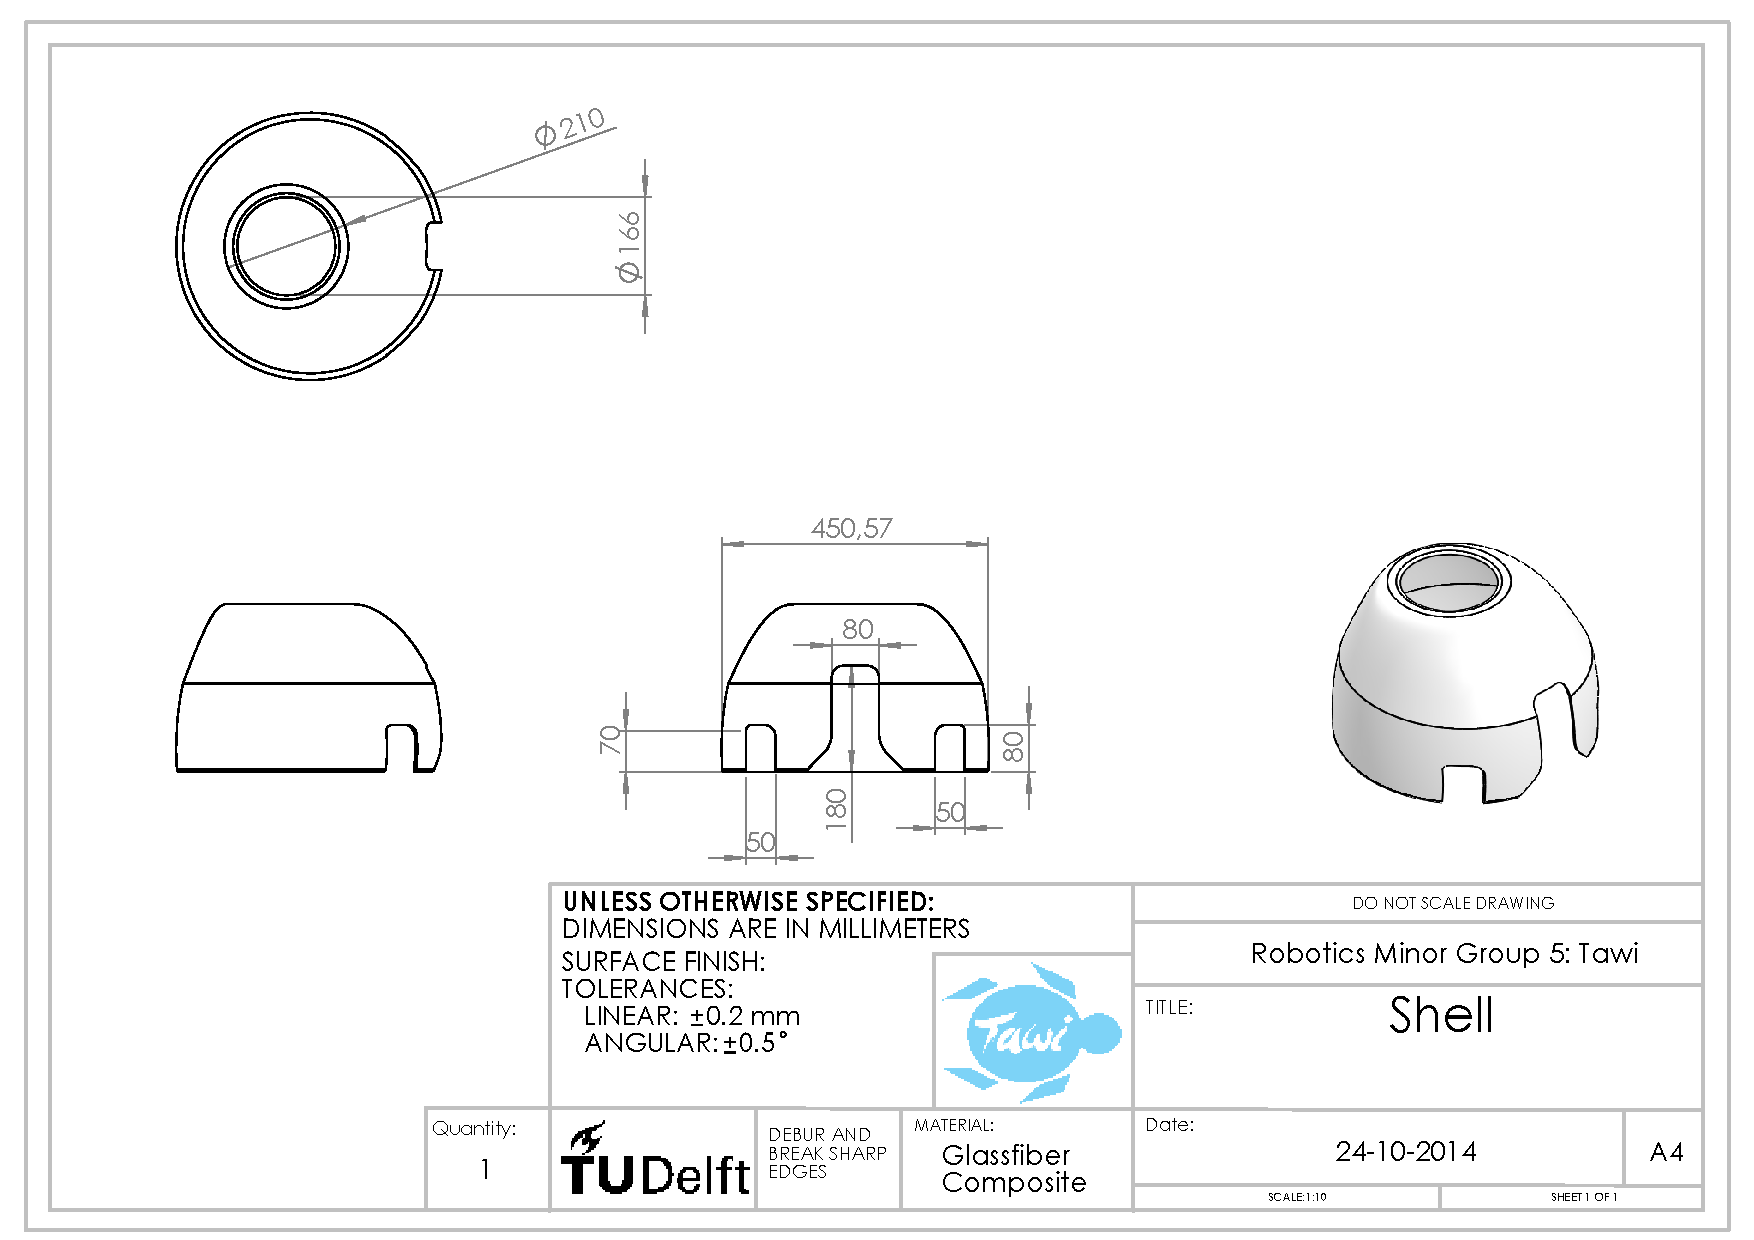
\includepdf[pages={1},landscape=true]{pdfdrawings/Shell.PDF}
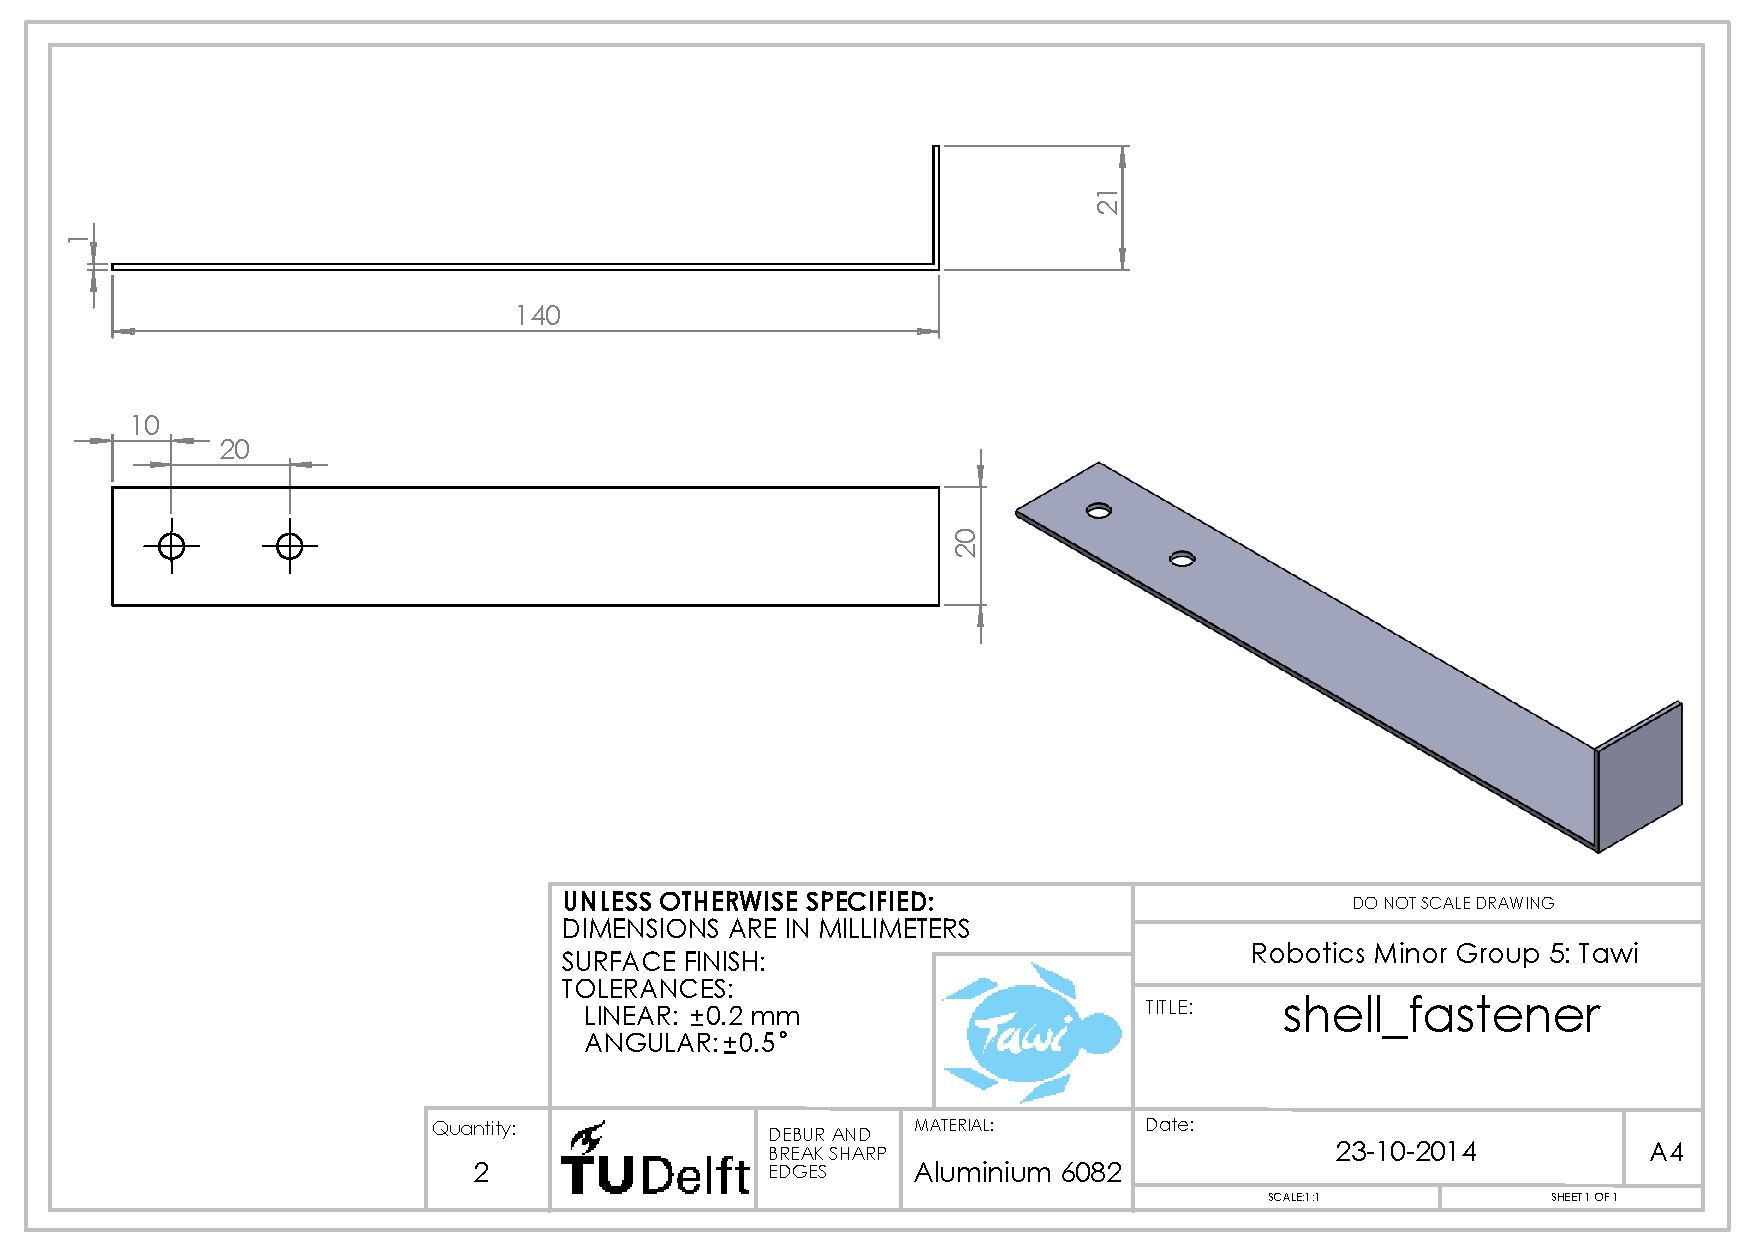
\includepdf[pages={1},landscape=true]{pdfdrawings/shell_fastener.PDF}
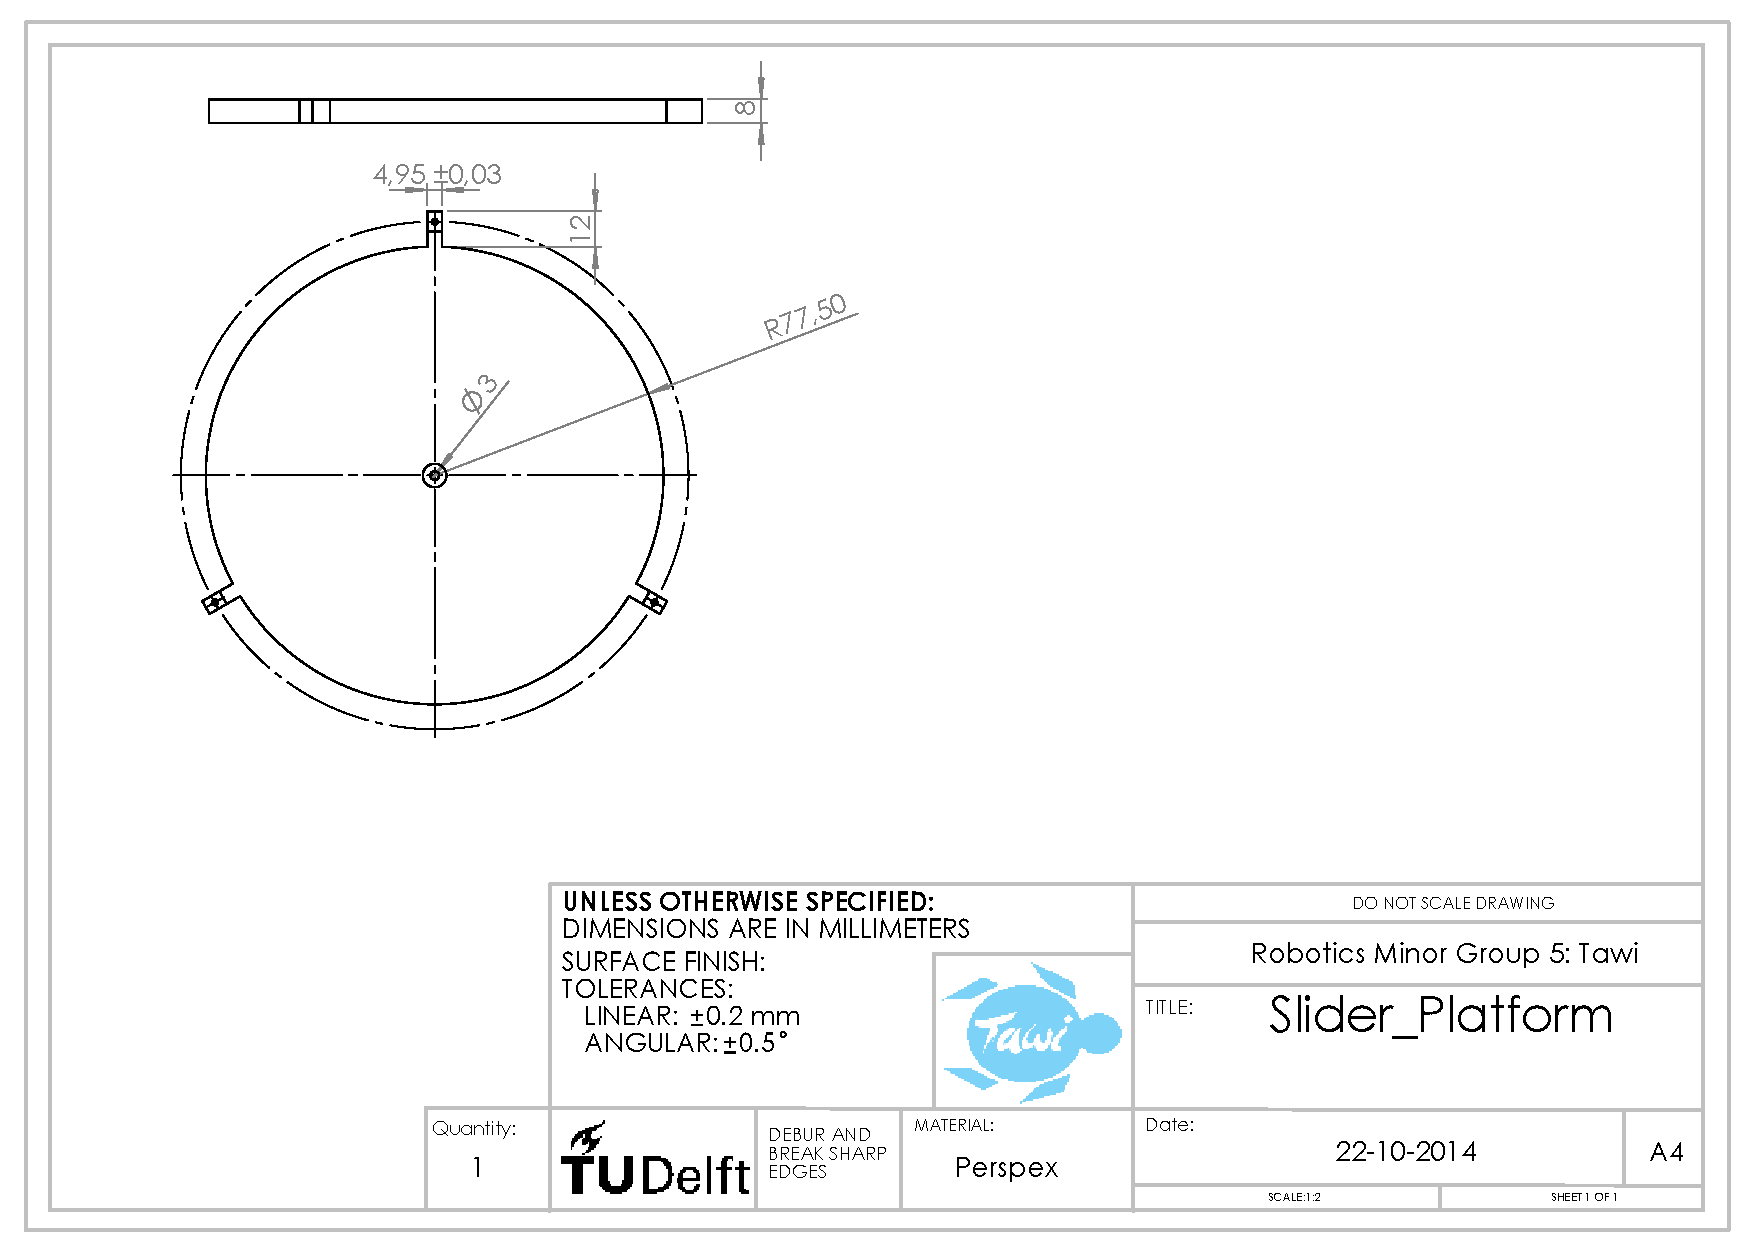
\includepdf[pages={1},landscape=true]{pdfdrawings/Slider_Platform.PDF}
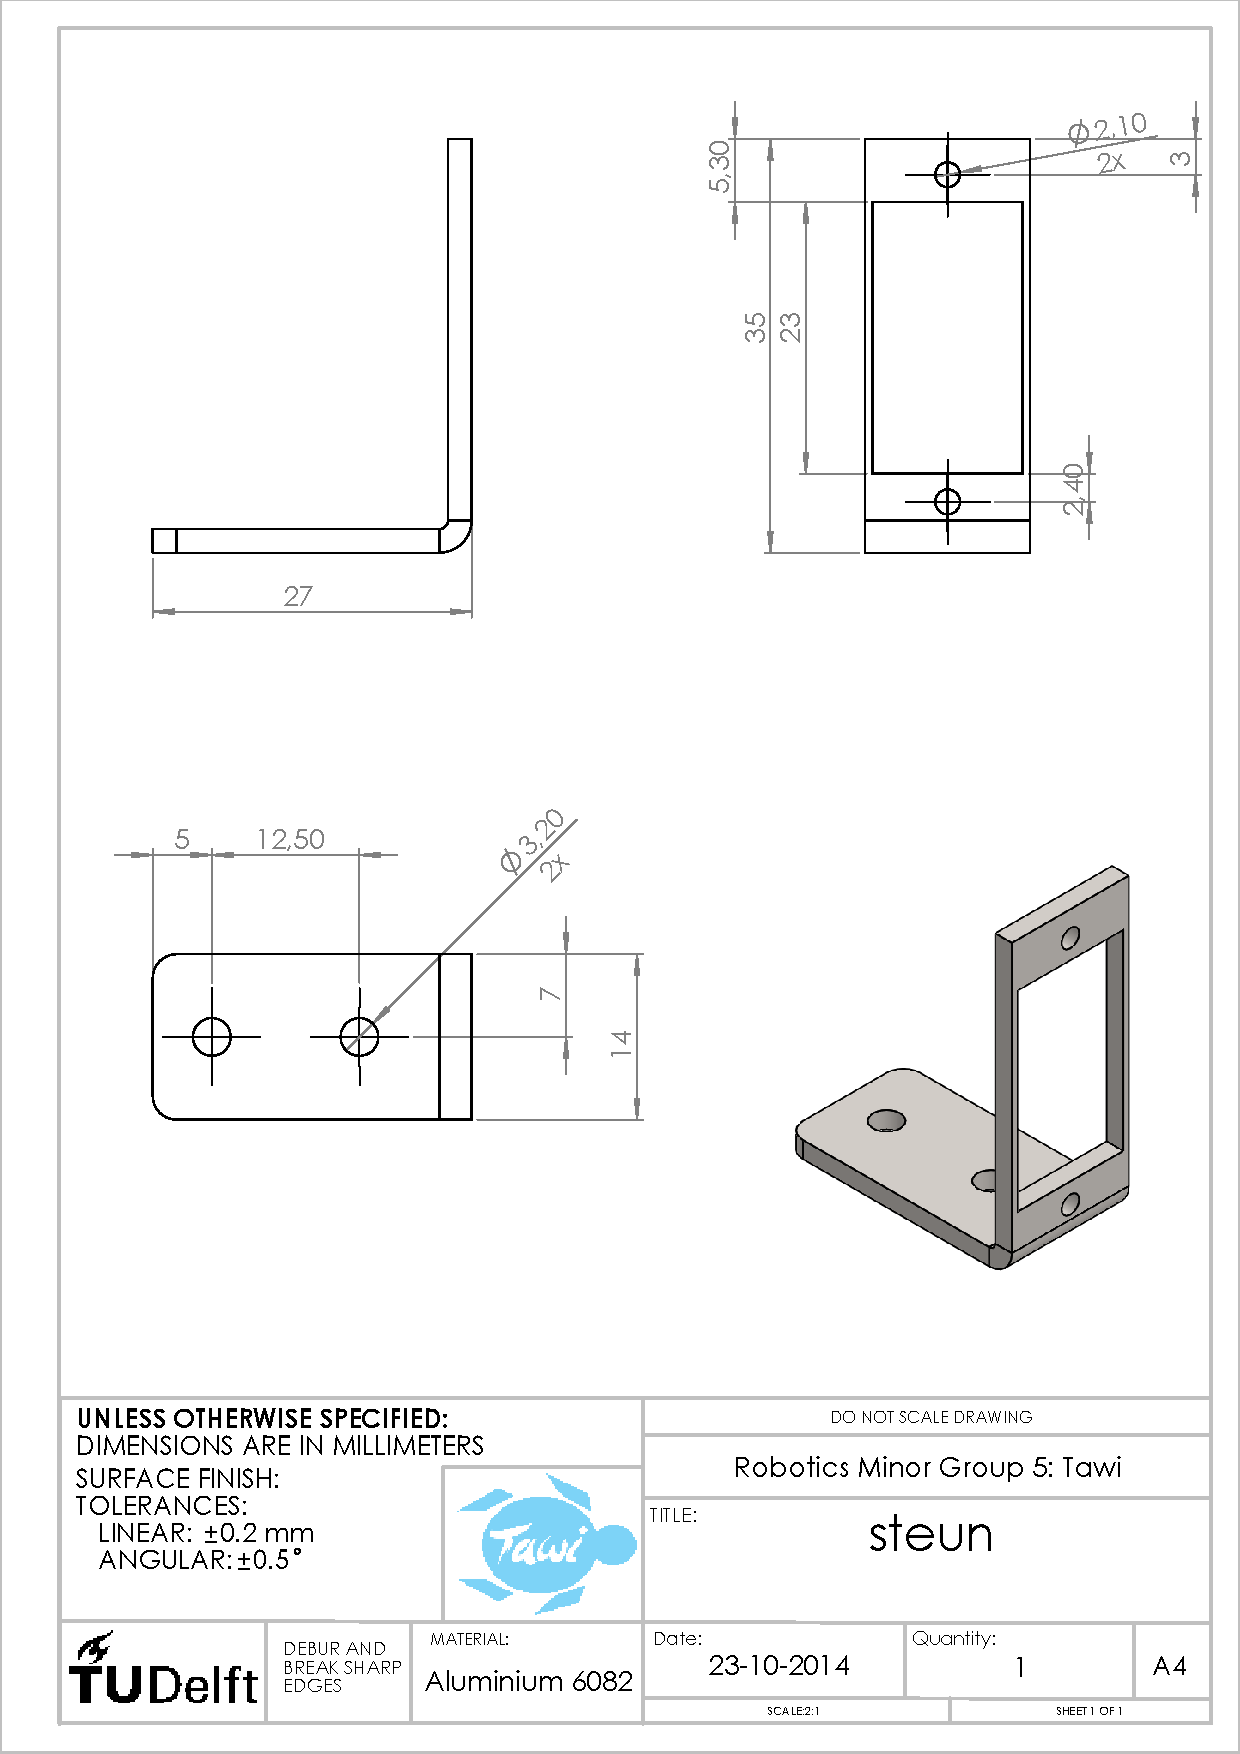
\includepdf[pages={1}]{pdfdrawings/steun.PDF}
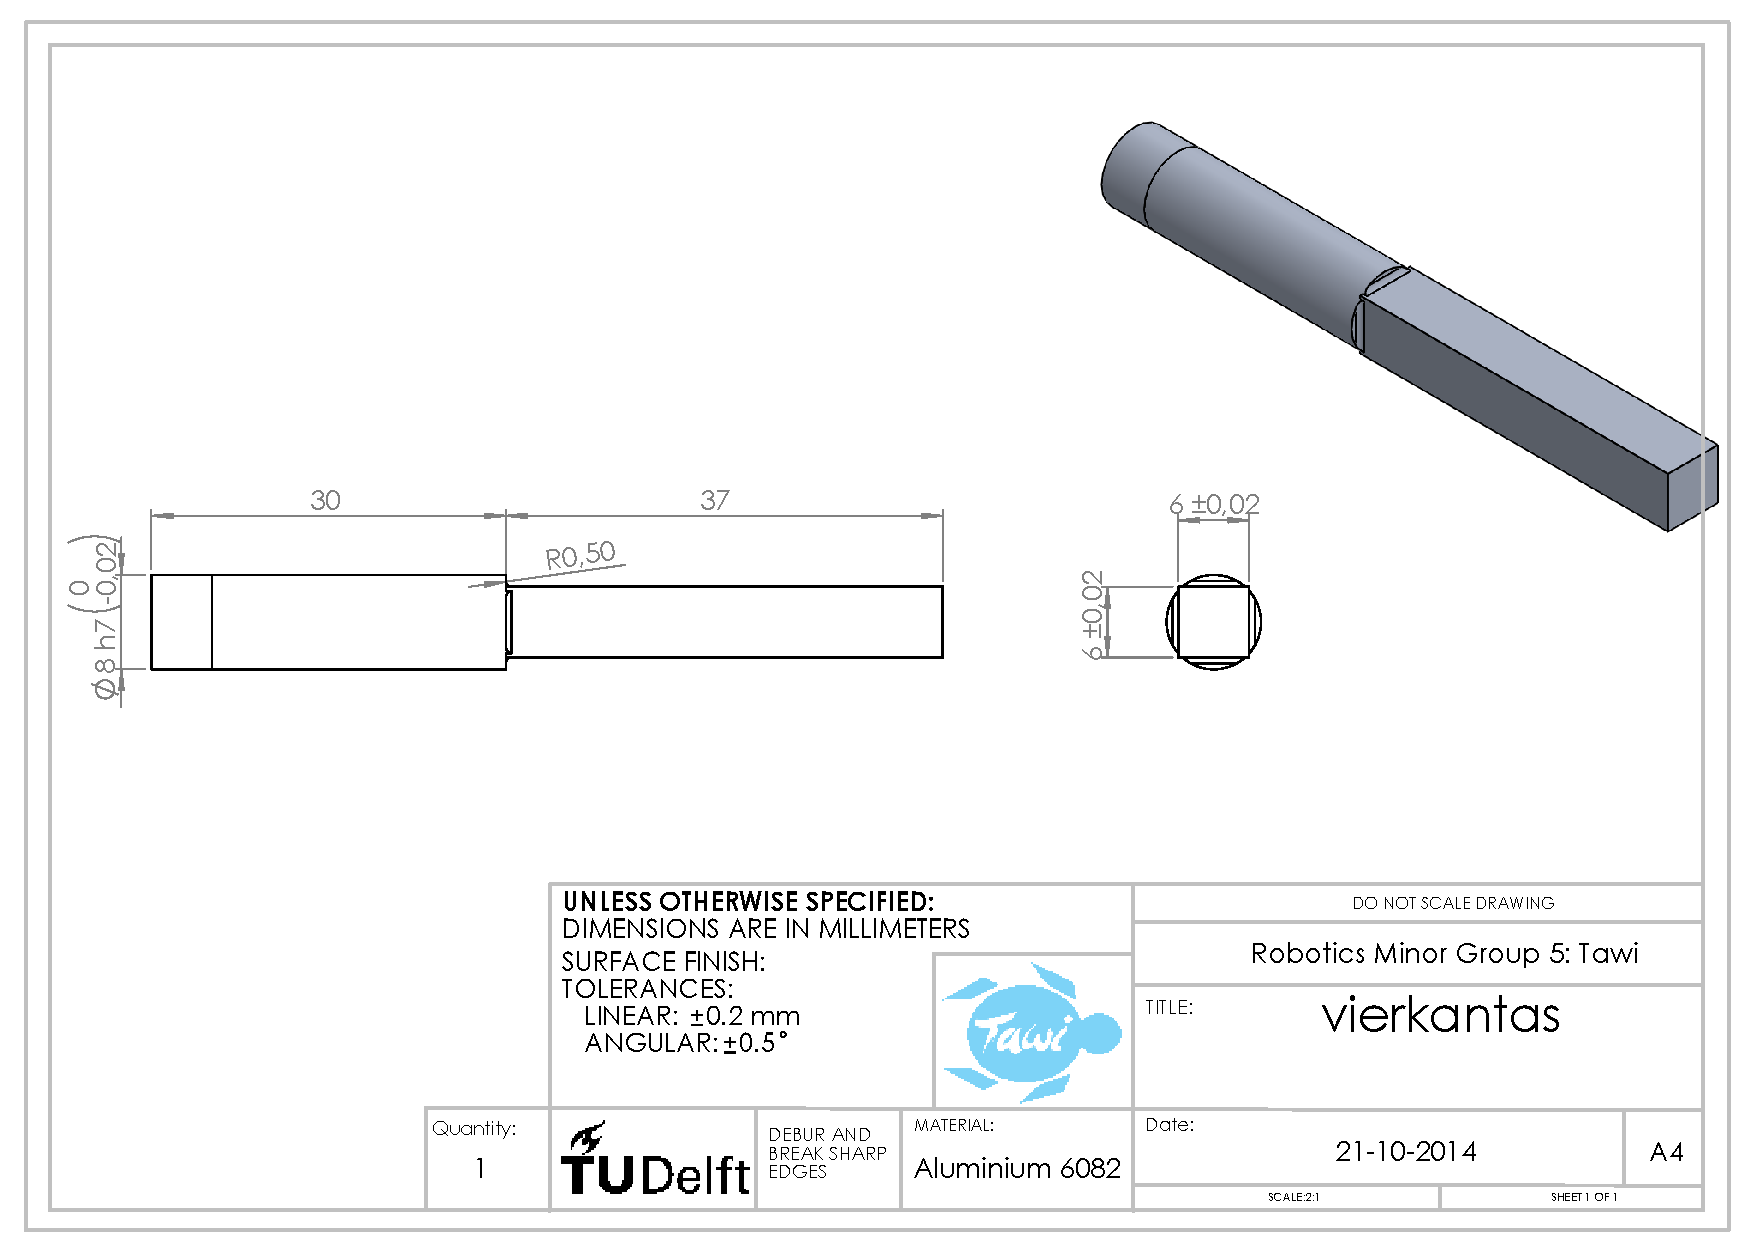
\includepdf[pages={1},landscape=true]{pdfdrawings/vierkantas.PDF}
\end{appendices}


\end{document}